
%\date{\today}

%\begin{abstract}
%Enhanced sampling methods, such as forward flux sampling (FFS), hold a great deal of promise for accelerating stochastic simulations of nonequilibrium biochemical systems involving rare events. However, the description of the tradeoffs between simulation efficiency and error in FFS remains incomplete. We present a novel and mathematically rigorous analysis of the errors in FFS that, for the first time, covers the contribution of every phase of the simulation. We derive a closed form expression for the optimally efficient count of samples to take in each FFS phase in terms of a fixed constraint on sampling error. We introduce a new method, forward flux pilot sampling (FFPilot), that is designed to take full advantage of our optimizing equation without prior information or assumptions about the phase weights and costs along the transition path. In simulations of both single- and multi-dimensional gene regulatory networks, FFPilot is able to completely control sampling error. Higher dimensional systems have additional sources of error and we show that this extra error can be traced to correlations between phases due to roughness on the probability landscape. Finally, we show that in sets of  simulations with matched error, FFPilot is on the order of tens-to-hundreds of times faster than direct sampling, in a fashion that scales with the rarity of the events.
%\end{abstract}

%\chapter{Automatic error control during forward flux sampling of rare events in master equation models}

\section{Introduction}

%Advances in single-cell and single-molecule techniques continue to produce new details about the individual biomolecules \supercite{Liu:2015jh,Vera:2016gm,Locke:2009gx,Muraro:2016hs,Li:2011kz}. Likewise, modeling efforts have progressed toward the goal of reconstructing complete cellular networks\supercite{Macklin:2014et,Karr:2015ej}. However, work is still needed to understand the dynamics of cells

Understanding how inanimate biochemical molecules come together and interact to form a living cell is one of the fundamental goals of biology\supercite{Harold:2003uu}. The cell's state can be described as a point in a high dimensional space, where each dimension corresponds to the concentration of a different molecule. Complex, nonequilibrium regulatory and signaling networks connect these molecules through positive and negative interactions, naturally resulting in a large number of metastable states within the space\supercite{Zhou:2012fc},  representing different cellular phenotypes. Projected into two dimensions, the phase space appears as a rough landscape, sometimes referred to as a quasipotential\supercite{Zhou:2012fc}, epigenetic\supercite{Waddington:1957ub}, or phenotypic\supercite{Nichols:2011cb} landscape. Stochastic fluctuations cause the cell's state to move along the landscape and occasionally jump between metastable states.

%It is now possible to describe the entire biochemical network (\ie the complete set of interacting pathways) underlying many different cellular activities.

%In particular, stochastic modeling is able to accurately capture the effects of fluctuation and variation (\ie intrinsic and extrinsic noise) on network behavior\supercite{Roberts:2011cs}. This makes stochastic modeling well suited to the simulation of switchable systems such as gene regulatory networks (GRN)\supercite{Hinman:2014bo,Borotkanics:2014hw,Barnes:2016gm,Gardner:2000bm}.

%As a tradeoff for its high accuracy and single molecule resolution, stochastic modeling is computationally expensive\supercite{Gillespie:2007bx}. Rare events (events for which the probability of occurrence is much lower than the most likely events, typically by several orders of magnitude) in particular pose a computational challenge for stochastic simulations\supercite{Becker:2012ej}. In the context of biochemical networks, rare events typically arise from the metastable dynamics of the collective action of many elementary reactions\supercite{Baron:2017tf}. For example, one common rare event is the switch from a state of low expression protein expression to a state of high protein expression\supercite{Choi:2010ge}. This kind of switching event can be found in many different genetic regulatory networks (GRN), such as those underlying the lysis/lysogeny decision in phage $\lambda$\supercite{Cao:2010dp} and the \it{lac} operon in \it{E. coli}\supercite{Roberts:2011cs}. A great number of elementary reactions, such as binding/unbinding of various species, are typically required before enough transcription factor is activated to shift the GRN towards the high expression state\supercite{Becskei:2005cs}. Each computational step of a stochastic simulation corresponds to a single elementary reaction\supercite{Gillespie:1976bj}. Thus, on average a great many computational steps are needed in order to observe a single rare event in a simulation trajectory.

Metastable systems, because they depend upon random fluctuations, are typically modeled using a formulation of the chemical master equation\supercite{Qian:2010if,Roberts:2015iu} or using stochastic differential equations\supercite{Wu:2013dx}. In the former case, the models are often numerically studied using the stochastic simulation algorithm\supercite{Gillespie:1976bj,Gillespie:2007bx} (SSA) or one of its many varieties\supercite{Bratsun:2005cs,Cao:2004cu,Gibson:2000jq}. Such simulations have provided insight into diverse biological processes, including: the lysis/lysogeny decision in bacteriophage $\lambda$\supercite{Cao:2010dp}, the \textit{lac} operon in \textit{Escherichia coli}\supercite{Roberts:2011cs},  check-pointing during the cell cycle\supercite{Li:2014iw}, differentiation of stem cells\supercite{Zhang:2014bu}, the binding of an intrinsically disordered peptide to a protein\supercite{Zwier:2016fx}, macrophage regulation\supercite{Smith:2016gj}, and gradient detection during yeast mating\supercite{Sharma:2016gw}.

%Although a number of approximation methods have been developed for skipping over the work of simulating the interstitials, for a long time it was thought that the accurate stochastic simulation of rare events required the simulation of every common event in between. Recently a class of advanced statistical techniques have emerged that promise to speed up the simulation of biochemical networks that include rare events. Collectively these techniques are known as \abr{ES}.  \abr{ES} can be thought of broadly as an extension of rare event sampling techniques, such as umbrella sampling, into the nonequilibrium domain (to which most biochemical networks belong). All \abr{ES} methods proceed along the same basic lines. First, the state space of the system (\eg the possible copy numbers of the biochemical species) under study is subdivided into a set of bins. Many separate simulations are then executed with starting and stopping conditions based on the boundaries of those bins, with an eye towards biasing the overall occupancy of said simulations towards regions of interest in the state space. Advanced statistical techniques are then used to unweight the collective simulation outcomes so as to calculate results equivalent to those obtained via unbiased simulation.

Transitions between metastable states in stochastic biochemical systems are infrequent in that one must wait a long time to observe a large fluctuation that causes the system to switch states\supercite{Baron:2017tf}. The time spent in the transition region is also very short relative to the waiting time\supercite{Becker:2012ej}. Such dynamics are known as rare events, and are expensive to simulate as most of the computational effort is spent simply simulating the waiting state. Numerical methods for improving the efficiency of simulating rare events, generally known as \abr{ES} techniques, have a long history. The earliest work in the field is typically credited to Kahn \etal{}\supercite{Kahn:1951es}, but has since been applied to the study of many systems in molecular mechanics. The key assumption is that metastable systems exhibit a large barrier separating the states on some free energy landscape. By biasing the simulation toward the transition path between the states one can more efficiently recover its free energy profile and, thus, the transition rates. For example: umbrella sampling\supercite{Torrie:1977hs,Souaille:2001gm} uses overlapping biasing potentials to confine multiple simulations to narrow windows along the path; metadynamics\supercite{Laio:2002ft,Dama:2014ef} gradually adds a repulsive potential to low points on the free energy surface causing the system to explore low probability regions of phase space and to eventually cross the barrier; transition path sampling\supercite{Dellago:1998kw,Crooks:2001cf,Jung:2017jj} generates a statistically correct set of transition paths starting from an initial trial path using acceptance and rejection criteria; weighted ensemble\supercite{Huber:1996dna,Zuckerman:2017eq} runs multiple independent trajectories while dynamically splitting and merging them, with careful accounting of the trajectory weights, to balance simulations along the transition path. In general, a final unbiasing and/or recombination step is always needed to calculate unbiased statistics.

Although stochastic biochemical systems are described by quasipotential rather than free energy landscapes, the underlying physics is compatible with \abr{ES}. Consequently, many varieties of \abr{ES} can be applied to stochastic biochemical systems with rare event dynamics. Three of the most well known candidates are \abr{FFS} \supercite{Allen:2005wy,Allen:2006cp,Valeriani:2007hv,Allen:2009kb}, nonequilibrium umbrella sampling\supercite{Warmflash:2007dz,Dickson:2009gt,Dickson:2009fua}, and weighted ensemble\supercite{Zhang:2010kfa,Bhatt:2010df,Adelman:2013ii,Donovan:2013gz,Donovan:2016bi}. Although much discussion has taken place regarding the strengths and weaknesses of each of these methods\supercite{Dickson:2010gf,Escobedo:2009dya} there is no consensus as to an optimal approach. In the case of a transition between only two metastable states along a single order parameter, \abr{FFS} appears to be a reasonable choice and is the focus of this work.

The \abr{FFS} method can be used to calculate both the transition rate, \ie, the inverse of the \abr{MFPT}, between two metastable states and the probability distribution along the transition path\supercite{Valeriani:2007hv}. Although it can be applied to non-stationary processes\supercite{Becker:2012fl}, here we investigate only stationary processes. The fundamental operation of \abr{FFS} is to partition the phase space along an order parameter using a series of non-intersecting interfaces that track progress over the transition barrier. Many trial trajectories are started successively from each interface in order to compute the probability of advancing to the next interface versus returning to the initial state. The product of the advancement probabilities and the probability flux out of the initial state gives the mean transition rate.

%The current literature leaves open many questions about the formal mathematics and error statistics of \abr{ES}. Of these open questions, the most essential is this: when accuracy is controlled for, is \abr{ES} truly faster than \abr{DS} (\ie the standard stochastic simulation method)? If so, for what models, and under what conditions? We sought to develop answers for these questions in the form of mathematical proofs, focusing our efforts on the \abr{FFS} method. Our strategy was to find formal expressions for the computational effort required to produce a simulation of a given accuracy for both the \abr{DS} and \abr{FFS} methods, and then draw conclusions from a comparison of the two.

%All existing studies looking at the relative speedup of \abr{ES} simulation over \abr{DS} simulation either do not control for accuracy\supercite{Allen:2005wy}, or are based on empirical results from simulations of one or two model systems that can only be applied narrowly to those specific systems\supercite{Donovan:2013gz}, or both. Previous work done by Allen and coworkers is suggestive of a possible path towards a more general statement about speedups. They found an analytical expression that can be used to predict the variance of the result (a proxy for simulation error) of an \abr{FFS} simulation given the computational effort expended in each of an \abr{FFS} simulation’s separate phases. In order to answer our question of interest about the speed of of \abr{FFS} simulation, the next step is to find a way to predict the computational effort required to produce a simulation of a given accuracy, or in other words the inverse of Allen’s expression. However, there are many possible equations for the inverse, as there are many ways to distribute computational effort amongst the various phases of an \abr{FFS} simulation such that the same simulation error is achieved. This is an example of the classical inverse problem that occurs with overdetermined equations in many fields of physics.

The generation of many trial trajectories at each of the interfaces is a large part of the computational work in \abr{FFS}. It is not surprising, then, that a number of authors have tried to optimize performance of \abr{FFS} by studying the interplay between the number of trajectories sampled and the statistical error. Allen {\etal}\supercite{Allen:2006ch} first introduced a framework for studying the relationship between error in the estimated transition rate constant and error in the estimated interface trial probabilities. They also studied the computational efficiency of \abr{FFS}, taken to be the inverse of cost times error, and showed that it was relatively insensitive to the choice of interface parameters. Borrero and Escobedo\supercite{Borrero:2008il} presented two techniques to minimize \abr{FFS} error for a fixed cost either by optimizing the number of trial runs at each interface or by iteratively refining the placement of the interfaces. Kratzer {\etal}\supercite{Kratzer:2013fs} extended this idea with an algorithm to automatically define interface number and position on-the-fly by constraining the number of successful trials to be the same for each interface. However, none of these previous works included a systematic treatment of the error arising from the estimate of the flux out of the initial state and they all assume that computational cost per unit distance along the order parameter is fixed. Jian {\etal}\supercite{Jiang:2013jc} later showed that interface placement along a complex transition landscape, {\eg} one with a metastable intermediate state, cannot be correctly optimized by methods that assume cost is proportional to interface distance.

%Using a novel derivation, we found a generalization of Allen's $\left( \mathsf{effort} \rightarrow \mathsf{error} \right)$ relation that predicts the complete distribution of the simulation result, not just the variance\footnote{Further, our version of the expression is more complete, as it includes the contributions of an important source of error (sampling error in the initial \abr{FFS} phase) that Allen did not consider.}. We worked around the inverse problem by using variational calculus to find the unique inverse of our expression that gives the minimum computational effort required to achieve a given level of error in a simulation. The ultimate product of this mathematical work is a set of simple, closed-form equations that we collectively call the \abr{FFS} Optimizing Equation (FFSOE). The FFSOE can be used to determine the phase-by-phase simulation plan that will achieve a given error goal (in terms of a desired upper bound on the percent error of the simulation result) using the least possible computational effort. We derived a number of subsequent results from the FFSOE. Most importantly, we define an exact mathematical criterion under which it is possible for \abr{FFS} to be faster than \abr{DS}, and show how to calculate the actual speedup factor.

%We also introduce \abr{FFPilot}, a novel \abr{ES} method based around the FFSOE. Compared to standard \abr{FFS} simulations, \abr{FFPilot} simulations run faster and are easier to set up. \abr{FFS} requires a user to specify a large set of unconstrained parameters (the number of trajectories to run in each separate phase) with no particular guidance. In place of these many parameters, \abr{FFPilot} requires only a single error goal, from which the runs per phase are determined in an automated and optimized way. We present the results of extensive testing of our parallelized implementation of \abr{FFPilot} (written in C++ using the MPI parallelization framework) on several different model systems of physical and biological processes. For a given level of simulation accuracy, we show that the computational effort that the FFSOE specifies either exactly matches the effort that is actually required, or is a monotonic bound on the effort, depending on the model being simulated. We show that a form of landscape correlation error is sufficient to explain the anomalous extra error that is not predicted by the FSSOE.

Here we present a method to optimally perform an \abr{FFS} simulation of a nonequilibrium stationary process at a given margin of error and confidence interval. The key advance of our method is to estimate all of the interface probabilities and costs from a short pilot simulation and then use those parameters to optimize the configuration of a full \abr{FFS} simulation. We minimize the total computational cost to achieve a user specified statistical error, which greatly reduces the number of choices that need to be made by the user. Our method includes a new formal treatment of the sampling error arising in the calculation of the flux out of the initial state, which is shown to have a significant influence on total cost. Unlike previous efforts, the cost in our method varies by interface, which enables it to account for changes in computational efficiency along the order parameter. We evaluate the capability of our method to control sampling error on three different models exhibiting rare event dynamics. In two one-dimensional models, sampling error dominates and is controlled precisely while in a multidimensional model landscape error becomes significant and requires oversampling. Finally, we derive an expression for the speedup of \abr{FFS} relative to direct simulation for the same level of error and show that the advantage of \abr{FFS} is substantial and increases with the rarity of the event.

The remainder of this work is organized as follows: In \secref{sec:methods} we introduce our theoretical framework for estimating the sampling error in a \abr{FFS} simulation. In \secrefTwo{sec:opteq_derivation}{sec:ffpilot_definition} we derive the optimizing equation used by our method to control sampling error and then describe the \abr{FFPilot} algorithm. In \secrefRange{sec:rem}{sec:gts} we evaluate the accuracy and performance of our method using three increasingly complex models. In \secrefTwo{sec:landscape_error}{sec:oversampling} we analyze sources of error outside of sampling error. Finally, in \secrefTwo{sec:efficiency}{sec:speedup} we evaluate the theoretical efficiency and measure the performance of \abr{FFPilot}.


%As the experimental picture of the cell grows to accommodate data from more and more different kinds of single cell and single molecule experiments, it becomes more and more important that theoretical models achieve a commensurate level of accuracy\supercite{Macklin:2014et,Karr:2015ej}.
%
%The field of systems biology offers many choices for such a theorertical basis, each with their own strengths and weaknesses. Broadly speaking, there exists a spectrum of cell modeling techniques that run 
%
%In particular, stochastic modeling is able to simulate transitions that are dominated by the dynamics of low copy number species (in the case of GRNs, the transcription factors) in a theoretically rigorous fashion\supercite{Cao:2010dp,Golding:2015ft,Robb:2014io,Arkin:1998vy}. This is in contrast to most other available modeling methods (such as those based on deterministic differential equations).
%
%As theoreticians, we would ideally like to be able to build stochastic models of very large biochemical networks involving thousands of distinct chemical species and reactions. Unfortunately, stochastic simulation is very slow \todo{cite}, often to the point of impracticality. The standard stochastic simulation protocol is known as the Gillespie Algorithm \todo{}, or more eponymously as the Stochastic Simulation Algorithm (SSA). SSA is straightforward to use and is extremely accurate. However, even simulations of simple 2-state GRNs with fewer than 10 distinct biochemical species may require the equivalent of CPU years worth of computational effort. This is due to the large separation of the time scales between individual molecular events and the switching rate of the overall system (see Fig \todo{figure}). Essentially, in order to simulate what may be the relatively slow dynamics of a system as a whole, SSA must simulate every single molecular event, no matter how many. Thus, standard SSA is too slow for the study of many complex gene regulatory networks of interest. 
%
%One of the greatest strengths of the \abr{ES} approach is that it requires no new approximationsUnlike methods such as Tau Leaping that
%
%We began this study with the goal in mind of implementing a parallelized \abr{ES} framework within Lattice Microbes (LM). LM is an established stochastic simulation software package maintained by the Roberts Lab, and has been extensively optimized for running on
%both single machines and HHPC cluster environments. We began with FFlux, as this method seemed the most compatible with our existing framework. However, as we designed and tested several prototype implementations of FFlux in LM, we noticed a recurrent problem. When using simulations to estimate values such as a \abr{MFPT},  first  Whereas the error statistics of the traditional stochastic simulation methods
%
%In general, when running simulations using the traditional stochastic modeling methods, the statistics of the sampling error closely follow those of the equivalent in vivo experiment. For example, when determining the \abr{MFPT} between two states of a system, if the researcher decides that they want an answer accurate to within $\pm 1\%$ the number of transition event observations required can be estimated using a straightforward interval based approach.
%Building on previous work\supercite{Allen:2006ch,Borrero:2008il,Borrero:2009wj,Kratzer:2013fs}, Further, we use the FFlux optimization equation to prove that FFlux is
%
%To our knowledge, 
%
%We have developed a novel \abr{ES} method that we call \abr{FFPilot}. \abr{FFPilot} automatically formulates a simulation plan that minimizes computational effort while achieving a user-defined error goal.
%
%Using a novel derivation, we found a generalization of Allen's effort$\rightarrow$error relation that predicts the margin of error (\ie the confidence interval of the percent error 
%
%a version of our effort$\rightarrow$error relation that constrains the free parameters to the unique global minimum with respect to 
%
%From this starting point used techniques from variational calculus to find an expression for the minimum computational effort required to perform a simulation of a specified accuracy.  we determined an exact set of mathematical conditions under which \abr{FFS} simulation is faster than \abr{DS} simulation. As well,
%
%The current work focuses on the relationship between computational effort and simulation accuracy for both \abr{DS} (the standard stochastic simulation method) and \abr{FFS} (FFlux). The papers describing the various \abr{ES} methods all make claims that \abr{ES} can speed up simulations by at least several orders of magnitude (one Weighted Ensemble paper claims speedups as large as ${10}^{15}$ fold). However, Once error is controlled for, the question remains open: is \abr{ES} faster than \abr{DS} for all model systems under all simulation conditions? If not for all, then when. There is no mathematical proof in the extant literature that  simulation accuracy is proportional to computational effort for all types of stochastic simulation,  typically by a factor of several orders of magnitude (one paper claims speed ups ) In standard FFlux simulation, the count of independent
%
%Earlier work on FFlux error was done by Allen and coworkers\supercite{Allen:2006ch}. They showed how the computational effort expended in each phase of an FFlux simulation relates to the error of the overall simulation result, although their treatment only covers a subset of the phases of an FFlux simulation. Building on Allen's results, Borrero and coworkers derived a recursive-form expression that can determine a simulation plan that minimizes the error in the final result given a fix quantity of computational effort available to "spend" on the simulation.
%
%We have derived expressions relating error and computational effort in FFlux simulations, and have developed a new \abr{ES} variant that incorporates these expressions. We rederived Allen's result from first statistical principles, and in so doing found a generalization of the computational effort/error relation that covers all of the simulation phases.



\chapter{Automatic error control during forward flux sampling of rare events in master equation models}

%\documentclass[class=article, float=false, crop=false]{standalone}
%\documentclass[10pt,letterpaper]{article}
%
%\input{error_control_of_enhanced_sampling-header}
%
%\begin{document}
%\vspace*{0.2in}

\section{Theory and methods}
\label{sec:methods}

\subsection{Simulation of rare events in stochastic processes}
\label{sec:ds_es_description}
%\begin{odone}
%    \1 \abr{FFS} speeds up simulation by ratcheting state space along an order parameter
%    \1 Proceeds in three steps
%        \2 Choose order parameter
%        \2 Choose tiling
%        \2 Run one set of simulations per tile/phase
%    \1 Outputs equivalent to those produced by DS can be obtained via statistical analysis of the trajectory ensembles produced in each phase
%        \2 $\mfpttrue$
%        \2 Probability Landscapes
%\end{odone}

The standard stochastic simulation protocol, here referred to as \abr{DS}, proceeds in two iterated steps: 1) increment the system time with the time of the next stochastic event, 2) update the system state according to the event. These two steps are repeated until some predetermined stopping condition (simulation steps, simulation time, etc.) is reached, at which point the simulation is terminated. Repeated \abr{DS} simulation produces a data set from which ensemble average quantities can be estimated by straightforward averaging. Running more \abr{DS} replicates leads to increased accuracy.
	
As discussed above, \abr{DS} has the disadvantage that it requires a long simulation time to sample each rare event. Therefore, calculating rare event statistics is computationally expensive. \abr[Enhanced sampling (ES)]{ES} methods use a combination of constraints on simulation trajectories and statistical unbiasing methods in order to enrich the sampling of rare events. \abr[Forward flux sampling (FFS)]{FFS} is a popular \abr{ES} method that was initially proposed by Allen and coworkers\supercite{Allen:2005wy}. We implemented the \abr{FFS} algorithm as follows:
\begin{enumerate}    
	\item Choose two points of interest in the state space of the model system, $\statea$ and $\stateb$. These will serve as an initial and a final state for the simulation.
	\item Choose a one dimensional parameter $\oparam$ for which $\oparamfunc{\statea} \neq \oparamfunc{\stateb}$. If $\oparamfunc{\statea} > \oparamfunc{\stateb}$, swap $\statea \Leftrightarrow \stateb$.
	\item Choose a set $\left \{ \ifacez \comma \cdots \comma \ifaceI \right \}$ of interface values of $\oparam$ such that $\oparamfunc{\statea} < \ifacei < \oparamfunc{\stateb}$ for every $\ifacei$. We say that a trajectory has fluxed forward with respect to a $\ifacei$ when it crosses the interface traveling in the direction of increasing $\oparam$, and that it has fluxed backward when it crosses traveling in the direction of decreasing $\oparam$.
	\item Begin \abr{FFS} phase 0:
        \begin{enumerate}
            \item Execute a \abr{DS} trajectory initialized at $\statea$. If the trajectory fluxes forward across $\ifacez$, record the elapsed simulation time $\simtimesymb$ since the previous crossing event, and also record the state $\statex$. Multiple phase 0 trajectories can be executed in parallel.
            \item If the trajectory ever crosses the final interface $\ifaceI$, pause the tracking of the waiting time until the trajectory moves backward across $\ifacez$.
            \item Once $\samplecountx{0}$ samples of $\simtimesymb$ have been collected, terminate the trajectories and move to the next phase.
        \end{enumerate}
    \item Begin \abr{FFS} phase $\phase > 0$:
        \begin{enumerate}
            \item\label{item:ffs_phasegz_step1} Randomly choose a state $\statex$ from the collection of states at which any trajectory in the previous phase crossed $\ifaceimo$.
            \item\label{item:ffs_phasegz_step2} Execute a \abr{DS} trajectory initialized at $\statex$. Allow the trajectory to run until it either crosses $\ifacez$ back into $\statea$ or moves forward across $\ifacei$. Terminate the trajectory and record a trajectory outcome value, either 0 or 1, depending on whether the trajectory moved backward or forward, respectively. If the trajectory moved forward, add the endpoint, which will lie along $\ifacei$, to the set of states that will be used to initialize trajectories during the next phase.
            \item Repeat steps \ref{item:ffs_phasegz_step1}-b.
            \item Once $\samplecount$ trajectory outcomes have been collected terminate the phase. Every phase $\phase$ trajectory can be executed in parallel.
        \end{enumerate}
    \item The procedure for \abr{FFS} phase $\phase$ is then repeated for phase $\phase + 1$ (during which trajectories are launched from $\ifacei$) until the final phase, phase $\Phase$, is reached. Trajectories in phase $\Phase$ begin at $\ifaceImo$ and may move forward across $\ifaceI$ and into $\stateb$.
\end{enumerate}

The overall aim of \abr{FFS} is to ratchet a simulation from $\atob$ across state space. The immediate goal of each phase is to estimate a phase weight. During phase $\phase$, samples are taken from an observable $\phrv$ that behaves as a random variable. $\phrvz$ is the waiting time in between forward flux events across $\ifacez$, and each $\phrvgz$ is the final outcome (0 for fall back or 1 for flux forward) of each trajectory launched in that $\phase$. The phase weight $\pwtrue$ is defined as the true expected value of the random variable $\phrv$:
\begin{equation}
    \label{eq:pw_definition}
        \pwtrue = \E{\phrv} =
        \begin{cases}
            \Simtimeatoz & \text{if}\ i=0, \\
            \fluxprob & \text{otherwise,}
        \end{cases}
    \end{equation}
where $\Simtimeatoz$ is the expected waiting time in between $\ifacez$ crossing events, and $\fluxprob$ is the probability that a trajectory launched from $\ifaceimo$ (\ie launched during phase $\phase$) crosses forward past $\ifacei$ before it falls back behind the starting interface $\ifacez$. The phase weights can be used to reweight the output of an \abr{FFS} simulation so as to calculate unbiased statistics.

%In the original version of \abr{FFS}\supercite{Allen:2005wy}, the phase 0 trajectories are terminated once a fixed simulation time $\Simtimefixed$ has elapsed. The number of forward flux events across $\ifacez$ during $\Simtimefixed$ are counted. We reformulated the algorithm in terms of $\samplecount$ instead of $\Simtimefixed$. This small change allows us to unify the sampling statistics of phase 0 with those of the other phases (see \secref{sec:phase_weight_moments}). We also found that the error in phase 0 inversely scales with the value of $\samplecount$ in a largely predictable fashion. Thus, the reformulation is also beneficial when running simulations of novel systems with unknown properties.

\subsection{Estimating values of interest from DS and ES stochastic simulations}
%\begin{odone}
%    \1 \abr{DS}
%        \2 the estimator of any ensemble average is the arithmetic mean of the appropriate observable taken over the appropriate time course or set of replicate simulations
%        \2 Exact description of full $\mfpttrue$ estimation protocol
%        \2 Exact description of full epigenetic landscape protocol
%    \1 \abr{FFS}
%        \2 The results of the biased and partitioned simulations carried out in \abr{FFS} can be recombined and reweighted into the unbiased ensemble averages using the appropriate weight factors
%        \2 We call the end of phase values the phase weights
%        \2 
%\end{odone}
As mentioned in the previous section, estimating values of interest from \abr{DS} simulation is straightforward. One valid estimator of any ensemble average quantity is simply the arithmetic mean taken across an appropriate set of direct observations. For example, in order to calculate the \abr{MFPT} of the switching process that takes some multistate system from $\atob$, $\samplecountds$ \abr{DS} simulations are initialized in $\statea$. Each of these $\samplecountds$ replicate simulations is allowed to run until the first time it enters $\stateb$, at which point it is terminated. The time that each simulation $\phase$ ran for is then a single sample $FPT_i$ of the first passage time of the switching process. The mean of these first passage time samples is an estimate of $\mfpttrue$\supercite{Gillespie:1981fo}:
    \begin{equation}
        \mfptestds = \frac{1}{\samplecountds} \sum^{\samplecountds}_{i=1} FPT_i,
    \end{equation}
where $\mfptestds$ is the estimator (\ie estimation function) of $\mfpttrue$ specific to \abr{DS} simulation. Throughout this paper, we place a $\;\widehat{}\;$ above a symbol to indicate that we are referring to an estimator of a value rather than to the value itself.

%A similar \abr{DS} simulation protocol can be used to calculate the probability density function (PDF) of a system. To calculate the PDF using \abr{DS}, a large number of simulations are run. The state of each trajectory is sampled at regular uncorrelated intervals. The state samples from all of the trajectories are then binned and normalized. The resulting normalized histogram is an estimator of the PDF. The total number of state samples taken determines the minimum probability that can be resolved.

Equivalent ensemble average estimators can be calculated using \abr{FFS}. Although the results of \abr{FFS} simulations are biased and partitioned, statistical protocols allow \abr{FFS} results to be recombined and reweighted so as to recapitulate the results of the unbiased ensemble. In order to perform these reweightings, we need estimates of the phase weights. During phase $\phase$ of \abr{FFS}, $\samplecount$ samples $\left\{ \phrvsampley{1} \comma \cdots \comma \phrvsampley{\samplecount} \right\}$ of an underlying random process $\phrv$ are taken. The mean of this sample can be used as an estimator $\pwest$ of phase weight $\phase$:
    \begin{equation}
    \label{eq:pwest_definition}
        \pwest = \frac{\sum_{\sample=1}^{\samplecount} \phrvsample} {\samplecount} =
        \begin{cases}
            \frac{\sum_{\sample=1}^{\samplecountz} \simtime}{\samplecountz}    & \text{if}\ i=0, \\
            \frac{\successcount}{\samplecount}    & \text{otherwise,}
        \end{cases}
    \end{equation}
where each $\simtime$ is a sample of the waiting time in between phase 0 forward flux events and $\successcount$ is the total count of trajectories that successfully fluxed forward during phase $\phasegz$.

In an idealized situation in which it were possible to know the exact values of the phase weights $\pwtrue$, the exact value of the $\mfpttrue$ could be found via a simple combination $\PWtrue$ of the phase weights:
    \begin{equation}
    \label{eq:PWtrue_definition}
        \mfpttrue = \frac{\Simtimeatoz}{\prod_{\phasegz} \fluxprob} = \PWtrueexp = \PWtrue.
    \end{equation}
In reality, we only know the phase weight estimators $\pwest$, so we must instead estimate the value of the $\mfpttrue$ by way of the combination of estimators $\PWest$:
    \begin{equation}
    \label{eq:PWest_definition}
        \mfptestffs = \PWestexp = \PWest.
    \end{equation}
where $\mfptestffs$ is the estimator of $\mfpttrue$ specific to \abr{FFS} simulation. Other quantities of interest, such as the stationary PDF, can also be calculated using the phase weights\supercite{Valeriani:2007hv}.

%In general, \abr{FFS} simulation returns biased results that can be transformed into unbiased results  by multiplying them with the appropriate combination of phase weights.

\subsection{Predicting simulation error in terms of margin of error}
%The observables of a stochastic simulations are not fixed, but are instead random variables, each with their own associated distributions. Each sample that is taken of an observable can be thought of as equivalent to taking a single draw from the distribution of possible observations. In order to calculate a statistic (eg mean, median, variance, etc.) of an observable, many samples are produced and then plugged into the appropriate estimator. These statistic estimates are in turn also random variables with distributions. Thus, error in the values of interest such as $\mfpttrue$ (which is the mean of a distribution of waiting times) can be quantified in terms of these estimate distributions.
%
%Often, stochastic simulations are run in order to calculate some statistic (eg mean, median, variance, etc.) of an observable of the system being modeled. Due to the nature of stochastic simulation, every time a set of simulations is run the calculated value of any statistic  value of, say, the $\mfpttrue$ (which is calculated as the mean of the waiting times) is produced,

Stochastic simulation results are not single valued, but are instead estimators, random variables with associated distributions. For example, when attempting to calculate $\mfpttrue$, each complete round of simulations can be thought of as performing a single draw from the distribution of possible $\mfptest$ values. A prediction about the likely level of error in any given set of simulations can be made based on the characteristics of this estimate distribution. One way to quantify confidence in this prediction is in terms of the margin of error. The margin of error of a random variable $X$ is defined as the ratio of half the width of a specified confidence interval and its expected value:
    \begin{equation}
    \label{eq:moe_definition}
        \moefunc{X} = \frac{\uboundfunc{X} - \lboundfunc{X}}{2 \E{X}},
    \end{equation}
where $\moefunc{X}$ is the margin of error of $X$ at confidence level $\alpha$, $\E{X}$ is the expected value of $X$, and $\lboundfunc{X}$ and $\uboundfunc{X}$ are the lower and upper confidence bounds, respectively. 

For many values of interest $\moefunc{X}$ is dependent on simulation parameters that are set by the user. For example, when calculating $\mfpttrue$, the margin of error $\moefunc{\mfptest}$ is dependent upon the total number of replicate simulations (when using \abr{DS}), or upon the count of trajectories run in each phase (when using \abr{FFS}).

%Thus, if the margin of error of $\mfpttrue$ can be determined, predictions can be made along the lines of ``$100 \cdot \alpha$ percent of the time, this given simulation protocol will produce an estimate of $\mfpttrue$ that will have no more than $100 \cdot \moefunc{\mfptest}$ percent error with respect to the true value''.

\subsection{Determining margin of error from simulation parameters}
\label{sec:moe_from_simulation_params}
It is straightforward to determine the margin of error of an estimator that depends on a single underlying observable. For example, consider the margin of error of an $\mfpttrue$ estimate as determined via \abr{DS} simulation, $\moefunc{\mfptestds}$. It has been shown that observations of first passage times between two well separated states follow an exponential distribution during \abr{DS} simulations\supercite{Becker:2012ej}. Given this distribution of first passage times, the central limit theorem\supercite{Olive:2014by} gives the distribution of $\mfpttrue$ estimates in the limit of large sample size:
    \begin{equation}
    \label{eq:fpt_clt_distribution}
        \frac{\sqrt{n} \left(\mfptestds - \E{FPT}\right) }{\sqrt{\V{FPT}}} \xrightarrow{D} \normdist{0}{1},
    \end{equation}
where $\samplecountds$ is the count of first passage time observations, $\E{FPT} = \mfpttrue$ is the expected value of the first passage time, $V[FPT]$ is the variance, $\normdist{0}{1}$ is the standard normal distribution (\ie mean 0 and variance 1), and $\xrightarrow{D}$ signifies that the distribution on the left converges to the one on the right. \eqref{eq:fpt_clt_distribution} implies\supercite{Olive:2014by} that an estimate of $\mfpttrue$ calculated using $\samplecountds$ observations will follow a normal distribution such that:
    \begin{align}
        \label{eq:mfptestds_moments}
        \begin{split}
            \E{\mfptestds} &= \mfpttrue, \\
            \V{\mfptestds} &= \frac{\V{FPT}}{\samplecountds} = \frac{\mfpttrue^2}{\samplecountds},
        \end{split}
    \end{align}
where the fact that $V = E^2$ for an exponential distribution was used to factor out $\V{FPT}$. The lower and upper bounds of the confidence interval of any normally distributed random variable $X$ can be found using a standard formula\supercite{Ross:2010wr} that depends on the first two moments of $X$:
    \begin{align}\label{eq:gaussian_ci_bound}
        \begin{split}
            \lboundfunc{X} &= \E{X} - \zscore \sqrt{\V{X}},   \\
            \uboundfunc{X} &= \E{X} + \zscore \sqrt{\V{X}},
        \end{split}
    \end{align}
where $\zscore$ is the z score associated with the confidence level $\alpha$ (\eg $\zscorex{.95} \approx 1.96$)\footnote{The z score $\zscore$ for any confidence level $\alpha$ can be calculated as $\zscore = \sqrt{2} \mathsf{Erfinv}\left( \alpha \right)$, where Erfinv is the Inverse Error Function\supercite{Carlitz:1963vu}, and $\alpha$ is expressed as a fraction. Some authors write the z score as $\zscorex{(1-\alpha)/2}$ instead of $\zscore$\supercite{Ross:2010wr}.}. Plugging \eqrefTwo{eq:mfptestds_moments}{eq:gaussian_ci_bound} into \eqref{eq:moe_definition} yields the margin of error of the \abr{DS} $\mfpttrue$ estimator:
    \begin{equation}\label{eq:moe_mfptestds}
        \moefunc{\mfptestds} = \frac{\zscore}{\sqrt{\samplecountds}}.
    \end{equation}
Thus, if say, $10^5$ replicate trajectories are produced during a \abr{DS} simulation, the resultant estimate of $\mfpttrue$ will have no more than $\frac{\zscorex{.95}}{\sqrt{10^5}} \approx \frac{1.96}{316} = 0.62\%$ difference from the true value 95\% of the time.

%for a wide variety of values of interest $X$, given that the distribution of $\est{X}$ obeys certain regularity conditions (mainly that $\E{\est{X}}$ and $\V{\est{X}}$ exist) \todo{REF}.

\subsection{Minimizing the computational cost required to achieve a desired error goal}
We define the computational cost $\Cost$ of a simulation to be equivalent to the average in-simulation time required to complete it (alternatively, one may use the count of simulation steps). When estimating $\mfpttrue$ using \abr{DS} simulation, the computational cost is:
    \begin{equation}\label{eq:cost_mfptestds}
        \Costds = \samplecountds \cdot \mfpttrue,
    \end{equation}
where $\samplecountds$ is the total number of replicate trajectories. \eqref{eq:moe_mfptestds} illustrates the direct tradeoff between computational cost and simulation accuracy. In order to find the minimum number of replicate trajectories that are required to achieve a particular error goal in \abr{DS} simulations, \eqref{eq:moe_mfptestds} can be solved for n:
    \begin{equation}\label{eq:ds_optimizing}
        \samplecountds = {\left( \frac{\zscore}{\moe} \right)}^{2}
        %n = \frac{\zscoresq}{\moefuncsq{\mfptestds}}.
    \end{equation}

%\subsection{Implementation of FFS with Lattice Microbes}
%\begin{odraft}
%    \1 We wrote and implementation of \abr{FFS} in Lattice Microbes, an open-source stochastic simulation software package produced by the Roberts lab. Lattice Microbes is a parallel program designed to run in both the desktop and the HHPC environments. It has been tested on clusters with thousands of CPU cores. To the best of our knowledge, our implementation of \abr{FFS} in Lattice Microbes is the first designed for high performance in a parallel cluster environment.
%\end{odraft}    
%
%Broadly speaking, \abr{ES} methods increase sampling of rare events by constraining simulation trajectories such that they spend more time in regions
%
%In general, the margin of error $\moe$ of an estimate $\est{x}$ of an ensemble average $x$ of some property $\mathfrac{x}$ is proportional to:
%\begin{equation*}
%	\moe \propto\limits_{n \rightarrow \inf} \sqrt{\frac{\V{\mathfrac{x}}}{\E{\mathfrac{x}}^2 n}} \\
%	\moe \propto\limits_{n \rightarrow \inf} \sqrt{\frac{\V{\mathfrac{x}}}{x^2 n}}.
%\end{equation*}
%In practice, what this means (among other things) is 
%
%\subsection{Measuring Simulation Error}
%\begin{odone}
%    \1 We quantify simulation error in terms of a relative margin of error.
%        \2 The relative margin of error of a random variable $X$ is defined as the ratio of half the width of a specified confidence interval and its expected value
%            \begin{equation}\label{eq:zeta_definition}
%                \zeta_{\alpha}\left[ X \right] = \frac{ub_{\alpha}\left[ X \right] - lb_{\alpha}\left[ X \right]}{2 \E{X}}
%            \end{equation}
%            \3 where $\zeta_{\alpha}\left[ X \right]$ is the relative margin of error at confidence level $\alpha$, and $lb_{\alpha}\left[ X \right]$ and $ub_{\alpha}\left[ X \right]$ are  the lower and upper confidence bounds, respectively.
%    
%    \1 When using \abr{ES} methods, there is also landscape error to consider
%        \2 All \abr{ES} methods involve sampling of some part of the simulated system's probability landscape
%            \3 Details of how error accumulates during the landscape sampling process vary between different \abr{ES} methods
%        \2 In \abr{FFS}, the landscape error affecting phase n depends on the probability landscape collected during phase n-1
%        \2 Thus, landscape error in phase n decreases as the number of trajectories run in phase n-1 increases
%        \2 Increasing number of runs in any phase also decreases sampling error, so there is no simple way to deconvolute landscape error and sampling error.
%\end{odone}
%
%We hypothesized that there must be some particular feature of the state space landscape of $\GTS$ that the simulations are exploring during phases 4 and 5 that is responsible for the anomalous error. We further reasoned that the same features that are responsible for what Allen and coworkers call landscape error could be responsible for the errors that we see here. In brief, Landscape error is due to two independent factors: 1) underrepresentation of regions of the landscape in the dictionary of trajectory starting points  at $\lambda_i$ (with respect to samples taken during a particular simulation), and 2) significant differences in $P\left(\lambda_{i}|\lambda_{i-1}\right)$ as a function of trajectory starting state. The total probability factor $P\left(\lambda_{i}|\lambda_{i-1}\right)$ that is measured in each phase $i>0$ can be thought of as a mixture of many independent probabilities, one for each state along $\lambda_{i-1}$, weighted by the (normalized) count of times the state is used as a starting point for a phase $i$ trajectory. If either of factors 1) or 2) occurs alone, $P\left(\lambda_{i}|\lambda_{i-1}\right)$ will still be correctly estimated. However, if the factors occur together they can lead to significant errors. In other words, if the landscapes assembled at $\lambda_3$ and $\lambda_4$ are heterogeneous across replicate simulations, and if differences in those landscapes can lead to differences in the effective value of $P\left(\lambda_{i}|\lambda_{i-1}\right)$, then landscape error may be the cause of the anomalous simulation error we observe in our simulations of $\GTS$. Of particular importance is the fact that the landscape error in phase $i$ is due to errors in the landscape assembled from the endpoints of successful trajectories launched during phase $i-1$. Thus, no amount of extra sampling performed during phase $i$ alone can completely abolish landscape error.
%
%\subsection{Controlling Simulation Error by Controlling Number of Runs}
%\begin{odraft}
%    \1 The dominant source of error in both DS and \abr{FFS} is sampling error
%        \2 For many simulation values of interest, such as $\mfpttrue$ and Probability Landscapes, error tends to decrease monotonically along with the total number of simulations run
%            \3 True for any value calculated as an average taken over a simulated ensemble, and for many values derived from such averages
%        \2 OPTIONAL: If an ensemble average is calculated a number of different times via independent repeated simulations, it will be seen to have a gaussian spread of values
%            \3 The mean will be the true ensemble value
%            \3 The spread (ie variance) will be proportional to the inverse square root of the number of runs in each separate simulation
%            \3 Can be shown to be true in general for ensemble averages (and for values derived from ensemble averages) via arguments based on the central limit theorem
%    \1 With DS, sampling error is controlled by a single parameter, how many replicates to run 
%        \2 Can be treated with established error statistics (exponential distribution)
%    \1 With \abr{FFS}, sampling error is controlled with N independent parameters, how many simulations to run in each phase
%        \2 More complicated than DS
%        \2 Some previous work has been done on the error statistics of both individual \abr{FFS} phase weights and on the overall outcomes of \abr{FFS} simulations
%            \3 phase 0 has been left out of all previously published treatments
%\end{odraft}
%
%As developers of stochastic simulations methods and software, we sought to develop a simulation protocol  One way to quantify 
%
%
%\subsection{Finding the Optimal Runs per Phase for a Given Error Goal}
%\begin{odraft}
%    \1 Given the known relationship between error and number of runs, variational calculus can be used to find the optimal (ie minimum) number of runs required to reach a certain error goal
%        \2 Method of Lagrange Multipliers
%            \3 Trivial for DS case
%            \3 \abr{FFS} case more complicated, need to minimize all phases together
%    \1 Resulting \opteq{} requires reasonable, conservative estimates of first and second central moments of the distribution of phase weight samples
%        \2 Moment estimation can be automated using new scheme, \abr{FFPilot}
%\end{odraft}
%
%\subsection{Models for testing}
%\begin{odraft}
%    \1 Toy model
%        \2 Simple set of random variable 
%    \1 SRG
%        \2 CME model
%        \2 Single species X, inhibitory Hill-like expression, 1st order decay
%        \2 Two states
%            \3 Low X
%            \3 High X
%    \1 GTS
%        \2 See \ref{fig:genetic_toggle_schematics}
%        \2 CME model consisting only of 1st and 2nd order reactions
%        \2 Seven species, single piece of operator DNA, cooperative binding to operator determines which protein is expressed
%        \2 Two states
%            \3 High A Low B
%            \3 High B Low A
%\end{odraft}
%
%\subsection{Derivation of model variants with different switching times}
%\begin{odraft}
%    \1 We wanted to explore how switching time effects accumulation of errors when using an enhanced sampling simulation method
%    \1 Began with versions of SRG and GTS from the literature, tried to find ways to adjust only switching time (with minimum overall perturabation)
%    \1 Self Inhibiting Gene
%        \2 Adjust switching time by adjusting hill coefficient
%    \1 genetic toggle switch
%        \2 Adjust switching time via novel protein churn parameter $\theta$
%        \2 Adjusting $\theta$ changes the transition path, but leaves the system as a whole unperturbed
%\end{odraft}
%
%\subsection{Statistics of Trajectory Ensembles}
%\begin{odraft}
%    \1 The statistics employed in this paper are based on the concept that repeated observations of some property of a stochastic system are equivalent to repeatedly sampling some random variable $\phrv$.
%        \2 The goal of a simulator is to produce an estimate of some value of interest $\omega$ based on samples taken from $\phrv$
%            \3 The estimate is produced from an estimator, a function of $\phrv$
%                \begin{equation*}\label{eq:estimator_definition}
%                    \widehat{\omega}\left[ \phrv \right]
%                \end{equation*}
%        \2 Estimators are typically distinguished from "true" value by the overhat notation 
%            \3 
%        \2 Estimators are themselves random variables, distinct from $\phrv$
%            
%        \2 Many different strategies for performing the sampling have been developed. We focus on two
%            \3 \abr{DS}
%            \3 \abr{FFS}, a type of Enhanced Sampling
%    \1 
%\end{odraft}
%
%\subsection{Estimation of Mean First Passage Time}
%\begin{odraft}
%    \1 In this paper we focus on achieving accuracy in one particular estimator, that of $\mfpttrue$.
%        \2 Although most of the methods and protocols we develop are already generalized.
%        \2 Two main reasons we focus on $\mfpttrue$
%            \3 Of critical importance in the study of rare events
%            \3 Central to the method of \abr{FFS}. In \abr{FFS}, all estimators are defined as products in which $\mfpttrue$ or one of its components is a factor.
%    \1 The procedure for estimating $\mfpttrue$ is somewhat different for the two sampling methods.
%        \2 In DS, there is a single simulation phase
%            \3 start a trajectory in state AA and wait (potentially a very long time) until it is absorbed in state BB.
%    \1 On the other hand, in \abr{FFS} there are
%    \1 As defined above, $MFPT_{DS}$ and $MFPT_{FFS}$ are equivalent only if the dwell time of the system in the starting state is much greater than the dwell time on the transition path
%        \2 This separation of time scales is characteristic of rare event systems \supercite{Becker:2012ej}
%\end{odraft}
%
%In this paper we focus on achieving accuracy in one particular estimator, that of $\mfpttrue$. Although many of the analyses and protocols developed in this paper can be applied in general to any estimator of a simulation observable.
%
%\subsection{Sources of Simulation Error}
%\label{sec:sources_of_error}
%\subsubsection{Direct Sampling}
%\begin{odraft}
%    \1 Sampling Error
%\end{odraft}
%\subsubsection{Forward flux sampling}
%\begin{odraft}
%    \1 Sampling Error
%    \1 Landscape Error
%\end{odraft}
%
%\subsection{Controlling Simulation Error by Controlling Margin of Error}
%\begin{odraft}
%    \1 
%\end{odraft}
%
%\subsection{Simulating Random Variables Using NumPy and SciPy}
%\begin{odraft}
%    \1 
%\end{odraft}
%
%\subsection{Stochastic Model of Genetic Toggle Switch}
%\begin{odraft}
%    \1 A generic model of a multi-state gene-regulatory biochemical network
%        \2 See fig \ref{fig:genetic_toggle_schematics}
%    \1 Contains a detailed representation of the dynamics of protein expression down to the single molecule level
%        \2 Although the particulars of transcription and translation are abstracted away
%    \1 Versions of the GTS have been built in live cells \supercite{Gardner:2000bm}.
%\end{odraft}

%\subsection{The Exclusive Genetic Toggle Switch}
%\begin{odraft}
%\1 (HAVE FIGURE: schematic diagram of toggle switch) The exclusive genetic toggle switch consists of a single piece of operator DNA that can produce two different proteins, A and B. The operator (and the system in general) stochastically switches back and forth between a high A state (\mc{A}), in which large quantities of A and minuscule quantities of B are produced, and a high B state (\mc{B}), in which the production rates are reversed. This rare switching event dominates the dynamics of this system. 
%\1 The binding of protein to the operator provides the basis for the state switching behavior. During the infrequent moments when the operator is unbound, both protein A and B are produced at an equal rate. Stochastically, a dimer of A or B will then bind to the operator, at which point only more of that same protein can be produced. The count of a protein determines the propensity of its binding to the unbound operator, so there is a strong positive feedback on binding.
%\1 To understand why the state switch is a rare event, it is instructive to realize that at some point during every switching event the count of the two proteins becomes equal. Thus, in order for a switching event from, say, $\mathcal{A}$ to $\mathcal{B}$ to occur, two events need to stochastically occur: a large quantity of protein A needs to be degraded without being replaced, and a large quantity of protein B needs to be produced without being degraded. Since either of these events occurring is unlikely, their co-occurrence is even more unlikely. 
%\1 In detail
%    \2 7 species, 14 reactions (NEED TABLE: species, reactions, rates)
%\1 (HAVE FIGURE: theta vs brute force $\mfpttrue$) Taking advantage of the relationship between switch frequency and protein production/degradation rates, we have designed a version of the GTS with a tunable switching frequency. We have multiplied every protein production and degradation rate in the system by a parameter $\theta$. A high value of $\theta$ leads to a high rate of protein turnover in the system, making switching much more likely, and a low value of $\theta$ has the opposite effect. Moreover, the ratio between the protein production and degradation rates is unaffected by $\theta$. This means that the steady state counts of A and B are for the most part also unaffected by $\theta$. Thus, we can tune the frequency of the rare switching event by altering $\theta$ without affecting the overall dynamics of the system. Remarkably, the switching frequency is linearly proportional to the choice of $\theta$.
%\end{odraft}
%
%\subsection{Modeling the Rare Switching Event as a Markov Process}
%\begin{odraft}
%\1 We assume that the rare switching event in the GTS system follows the dynamics of a two-state Markov model. This is a reasonable assumption given that the relaxation time of the system upon entering either \mc{A} or \mc{B} is much shorter than the mean time in between switching events (cite: Becker, 2012). In effect, imposing Markovian dynamics on the switching event is a sort of coarse-grained analysis of our molecular-detail simulations. This allows for the study and quantification of the switching event as an independent stochastic process. 
%\1 The waiting times in between state transition events in a Markov model are exponentially distributed. As with any exponential distribution, the waiting times are characterized by a single parameter, which in this case is the mean waiting time. A primary goal of the simulations discussed in this paper is to determine the value of this parameter for a given version of the GTS.
%\end{odraft}
%
%\subsection{Parameterizing the Rare Event Markov Process}
%\subsubsection{Connecting the CME Model and the Markov Model}
%\begin{odraft}
%\1 So far we have described two independent models of the GTS: a detailed CME model with a many-dimensional state space, and a coarse-grained two-state Markov model. We aim to take the outcomes of a set of simulated trajectories of the detailed model, which has been parameterized in terms of the elementary reactions of the GTS, and use them to parameterize the coarse-grained model. In order to connect the two models together we need two things:
%    \2 A 1D order parameter that describes the transition from one CME state to another. Simulation outcomes tend to be insensitive to the choice of order parameter, although a simulation using a "bad" order parameter may require more computational effort to achieve a given level of error.
%    \2 A state rule that will allow us to determine what single state a given CME trajectory is in at a given time. This rule effectively defines both the states themselves as well as the exact nature of the switching process. The choice of state rule can have an effect on the simulation outcome, as different rules effectively describe different switching processes.
%\1 (PROBABLY CUT THIS PARAGRAPH) There is no completely general, system-independent way to determine an appropriate order parameter. However, for systems with well-separated metastable states there is a straightforward protocol that can be followed to produce a reasonable order parameter:
%    \2 Either through prior knowledge or via one of the many estimation methods, determine the rough location of the system's stable fixed-points in terms of the system's full state space.
%    \2 Pick two states that you want to study the transition between. The steps that follow can be repeated if your system has more than two states.
%    \2 Determine the equation of the straight line that connects the two states.
%    \2 Now determine the general equation of all the possible lines (for a 2D state space), planes (for 3D), or hyperplanes (for nD) that lie perpendicular to your connecting line. Write out this equation in the form $c\sub{0} x\sub{0} + c\sub{1} x\sub{1} + ... + c\sub{n} x\sub{n} = d$ (given that $\left\{x\sub{0}, x\sub{1} ... x\sub{n}\right\}$ is your state vector, $\left\{c\sub{0}, c\sub{1} ... c\sub{n}\right\}$ is a set of constants, and $d$ is the variable that lets you choose among the possible perpendicular objects). The left hand side of this equation is your order parameter. This order parameter can then be further refined based on the particulars of your system and the aspects of it under study.
%\1 We characterize the transition event in the GTS system in terms of an order parameter $\Delta$. $\Delta$ is based on the difference of the total count of the two proteins in the GTS:
%\begin{align}
%	\Delta &= \mathrm{number\ of\ molecules\ of\ protein\ B} - \mathrm{number\ of\ molecules\ of\ protein\ A} \\
%	       &= (n\sub{B} + 2n\sub{B\sub{2}} + 2n\sub{OB\sub{2}}) - (n\sub{A} + 2n\sub{A\sub{2}} + 2n\sub{OA\sub{2}})
%\end{align}
%\1 Following the regions framework of Dinner (cite: Dinner 2010), we define each state in the CME by first choosing a value of $\delta$. This value is used to establish an interface which we will say separates that particular state from the rest of state space. The choice of $\delta$ value is somewhat arbitrary, but as long as it fulfills certain conditions:
%    \2 In between the two states we're studying.
%    \2 Close to but not on top of the stable fixed point.
%    \2 Far from the midpoint of the transition.
%\1 then the time-scale separation assumptions that underpin the Markov model will still hold. Any trajectory that passes through the interface of state \mc{X} while moving towards the stable fixed point is said to have transitioned into state \mc{X}. If that trajectory then passes back though interface \mc{X} but has not yet transitioned into a different state, it is said to be in the region of \mc{X}.
%\end{odraft}

%- Once we have the estimator mean and variance we can then calculate a confidence interval for the estimator. 
%    - system independent
%    -  why confidence intervals are appropriate for bounding behavior of single simulations
%    - Though somewhat more complicated to implement, RCI has the virtue of making simulations much easier to setup and run. Previously, a computationalist would have needed to specify upfront a set number of replicate simulations to run
%
%- 
%    - we have chosen to focus on $\mfpttrue$ in our error control efforts
%        - the scale parameter of the exponential distribution of time in between switching events
%        - (Most?) essential characteristic of any rare event systems
%        - required for calculation of other results of interest, such as the epigenetic landscape

%\end{markdown}

%\end{document}




%\documentclass[class=article, float=false, crop=false]{standalone}
%\documentclass[10pt,letterpaper]{article}
%
%\input{error_control_of_enhanced_sampling-header}
%
%\begin{document}
%\vspace*{0.2in}

\section{Results}

%\subsection{Predicting Margin of Error Via Sample Count}
%\begin{odone}
%    \1 We quantify simulation error in terms of a relative margin of error.
%        \2 The relative margin of error of a random variable $X$ is defined as the ratio of half the width of a specified confidence interval and its expected value
%            \begin{equation}\label{eq:moe_definition}
%                \zeta_{\alpha}\left[ X \right] = \frac{ub_{\alpha}\left[ X \right] - lb_{\alpha}\left[ X \right]}{2 \E{X}}
%            \end{equation}
%            \3 where $\zeta_{\alpha}\left[ X \right]$ is the relative margin of error at confidence level $\alpha$, and $lb_{\alpha}\left[ X \right]$ and $ub_{\alpha}\left[ X \right]$ are  the lower and upper confidence bounds, respectively.
%    
%    \1 When using \abr{ES} methods, there is also landscape error to consider
%        \2 All \abr{ES} methods involve sampling of some part of the simulated system's probability landscape
%            \3 Details of how error accumulates during the landscape sampling process vary between different \abr{ES} methods
%        \2 In \abr{FFS}, the landscape error affecting phase n depends on the probability landscape collected during phase n-1
%        \2 Thus, landscape error in phase n decreases as the number of trajectories run in phase n-1 increases
%        \2 Increasing number of runs in any phase also decreases sampling error, so there is no simple way to deconvolute landscape error and sampling error.
%\end{odone}
%
%As mentioned in the previous section, both \abr{DS} and \abr{ES} simulations can be used to estimate the $\mfpttrue$ between the states of a multi-stable system.
%
%The error characteristics of the \abr{DS} version of $\mfptest$ have been well described in  previous work. If the states of the system under investigation are separated such that the system as a whole spends much, much more time in one well-defined state or another than it does in transition between states, the dynamics of the state switching process will be equivalent to those of a Markov process. In that case, the waiting times in between switching events will follow an exponential distribution.
%
%
%
%\subsection{The Blind Optimization Method, for Independently Controlling Error }
%\label{sec:blind_optimization_description}
%Initially we devised a "blind" optimization method for determining the number of samples to take in each phase of \abr{FFS}. The method is blind both in the sense that no prior knowledge of the system is required, and in the sense that each phase is optimized independently of the others.

\subsection{Derivation of the \opteq{}}
\label{sec:opteq_derivation}
In this subsection we find the choice of number trajectories to launch in each \abr{FFS} phase (which we will also refer to as sample count or $\samplecount$) that will minimize simulation run time while fixing the margin of error $\moe$ of the estimator of \abr{MFPT}. We will refer to the $\mfpttrue$ estimator in this subsection as $\PWest$. The derivation of the optimal choice of $\samplecount$ starts with the characterization of the moments and distribution of $\PWest$. We then use the moments and distribution of $\PWest$ to find $\moe$ as a function of the per-phase sample counts $\samplecount$. We then use the method of Lagrange multipliers to find the optimal choice of $\samplecount$ that will keep $\moe$ fixed while minimizing simulation run time.

%The relationship we will derive is valid for the class of estimators that can be written as the product of one or more independent $\sqrt{n}$-consistent estimators of some function of simulation observables.

\subsubsection{The moments and distribution of the \abr{FFS} $\mfpttrue$ estimator $\PWest$}
\label{sec:phase_weight_moments}

%In distinguishing between exact values such as $\PWtrue$ and estimators such as $\PWest$, it is important to note that while $\PWtrue$ has a single true value, $\PWest$ is a random variable with a distribution of values.

Each individual \abr{FFS} phase weight $\pwtrue$ can be thought of as the first moment (\ie the mean) of an observable $\phrv$ of a random process that is specific to phase $\phase$. By the end of every \abr{FFS} phase $\phase$, $\samplecount$ samples have been drawn from $\phrv$ (see \secref{sec:ds_es_description} for a more concrete description), at which point the phase weight $\pwtrue$ is estimated as:
    \begin{equation*}
        \pwest = \frac{1}{\samplecount} \sum_{\sample=1}^{\samplecount} \phrvsample
    \end{equation*}
Given the above form of $\pwest$, and given that the observable $\phrv$ meets certain regularity conditions \supercite{Oehlert:1992gp}, the asymptotic distribution of the individual $\widehat{w}_i$ terms can be determined from the central limit theorem:
    \begin{equation}
    \label{eq:pwest_asymptotic_dist}
        \frac{\sqrt{n_i} (\widehat{w}_i - w_i)}{\sqrt{\pwvtrue}} \xrightarrow{D} \normdist{0}{1}.
    \end{equation}
The moments of each $\pwest$ can be determined by the appropriate interpretation of \eqref{eq:pwest_asymptotic_dist}:
    \begin{align}
    \label{eq:pwest_moments}
        \begin{split}
            \E{\widehat{w}_i} &= w_i, \\
            \V{\widehat{w}_i} &= \frac{\pwvtrue}{n_i}.
        \end{split}
    \end{align}
An estimator with this type of convergence behavior is said to be \ncon.

Given that the $\mfpttrue$ estimator $\PWest$ is defined in \eqref{eq:PWest_definition} as a function $g\left[ \pwestvec \right]$ of a vector of \ncon estimators $\pwestvec = \left\{ \pwestx{0} \comma \pwestx{1} \comma \cdots \comma \pwestx{N} \right\}$, we can apply the multivariate delta method\supercite{Wasserman:2013dt} to determine the moments and distribution of $\PWest$. From the multivariate delta method, we know that:
    \begin{equation}
    \label{eq:PWest_asymptotic_dist}
        \frac{\PWest - \PWtrueexpinv}{\sqrt{\PWtruegradtrans \Sigma \nabla_{\pwestvec}}} \xrightarrow{D} \normdist{0}{1},
    \end{equation}
%    \frac{\left( g \left[ \bm{\widehat{w}} \right] - g \left[ \bm{w} \right] \right)}{\sqrt{\nabla_{\bm{w}}^{T} \Sigma \nabla_{\bm{w}}}} \xrightarrow{D} \normdist{0}{1}
where $\PWtruegrad$ is the gradient of $g(\pwestvec)$ evaluated at $\pwtruevec$, $\PWtruegradtrans$ is the transpose of $\PWtruegrad$, and $\Sigma$ is the covariance matrix of the phase weight estimators $\pwest$. We can determine the moments of $\PWest$ by interpreting \eqref{eq:PWest_asymptotic_dist}:
    \begin{align}
    \label{eq:PWest_moments}
        \begin{split}
            \E{\PWest} &=\PWtrueexp = \mfpttrue, \\
            \V{\PWest} &= \PWtruegradtrans \Sigma \PWtruegrad.
        \end{split}
    \end{align}

A simpler form of $\V{\PWest}$ can be found. To begin with, we find $\PWtruegrad$. In column vector form it is:
    \begin{equation}
        \PWtruegrad =
        \begin{pmatrix}
            \pwtrueinvx{0}  \PWtrueexpaltinv  \\
            -\pwtrueinvx{1} \PWtrueexpaltinv   \\
            \vdots \\ 
            -\pwtrueinvx{\Phase}     \PWtrueexpaltinv
        \end{pmatrix} =
        \begin{pmatrix}
            s_0   \\ 
            -s_1    \\ 
            \vdots \\ 
            -s_{\Phase}
        \end{pmatrix},
    \end{equation}
where we have substituted $s_\phase$ for $\pwtrueinvx{\phase}  \PWtrueexpaltinv$ for the sake of brevity. If the covariance of $\pwest$ and $\pwestx{j}$ is written as $\sigma_{ij}$, then the covariance matrix $\Sigma$ is:
    \begin{equation*}
        \Sigma = 
        \begin{pmatrix}
            \sigma_{00}       & \sigma_{01}       & \cdots & \sigma_{0 \Phase} \\
            \sigma_{10}       & \sigma_{11}       & \cdots & \sigma_{2 \Phase} \\
            \vdots            & \vdots            & \ddots & \vdots            \\
            \sigma_{\Phase 0} & \sigma_{\Phase 1} & \cdots & \sigma_{\Phase \Phase}
        \end{pmatrix},
    \end{equation*}
and the variance of $\PWest$ can be written as:
    \begin{equation}\label{eq:PWest_variance_expansion}
        \V{\PWest} =
        \begin{pmatrix}
            s_0 & -s_1 & \cdots & -s_{\Phase}
        \end{pmatrix}
        \begin{pmatrix}
            \sigma_{00}       & \sigma_{01}       & \cdots & \sigma_{0 \Phase} \\
            \sigma_{10}       & \sigma_{11}       & \cdots & \sigma_{2 \Phase} \\
            \vdots            & \vdots            & \ddots & \vdots            \\
            \sigma_{\Phase 0} & \sigma_{\Phase 1} & \cdots & \sigma_{\Phase \Phase}
        \end{pmatrix}
        \begin{pmatrix}
            s_0    \\ 
            -s_1    \\
            \vdots \\ 
            -s_{\Phase}
        \end{pmatrix}.
    \end{equation}
If we impose the assumption of independence on all of the phase weight estimators $\pwest$, then only the diagonal elements of the covariance are non-zero:
    \begin{equation*}
        \V{\PWest} =
        \begin{pmatrix}
            s_0 & -s_1 & \cdots & -s_{\Phase}
        \end{pmatrix}
        \begin{pmatrix}
            \sigma_{00} & 0           & \cdots & 0           \\
            0           & \sigma_{11} & \cdots & 0           \\
            \vdots      & \vdots      & \ddots & \vdots      \\
            0           & 0           & \cdots & \sigma_{\Phase \Phase}
        \end{pmatrix}
        \begin{pmatrix}
            s_0    \\ 
            -s_1    \\
            \vdots \\ 
            -s_{\Phase}
        \end{pmatrix}.
    \end{equation*}
Under this condition of independence the form of $\V{\PWest}$ can be simplified considerably:
    \begin{align*}
        \V{\PWest} &= \sum_i s_i^2 \sigma_{ii}, \\
        \V{\PWest} &= \sum_i \pwtrueinvsqx{i} \sigma_{ii} \PWtrueexpaltsq,
    \end{align*}
and since $\sigma_{ii} = \V{\pwest}$:
    \begin{align*}
        \V{\PWest} &= \PWtrueexpaltsq \sum_i \frac{\V{\pwest}}{\pwtruesq}.
    \end{align*}
Finally, plugging in substitutions from \eqref{eq:PWtrue_definition} and from \eqref{eq:pwest_moments}, the variance of $\PWest$ is:    
    \begin{equation}\label{eq:PWest_variance}
        \V{\PWest} = \mfpttrue^2 \sum_i \frac{\pwvtrue}{\pwtruesq n_i}.
    \end{equation}

Alternatively, the variance of $\PWest$ can be derived from the formula for the variance of a product of random variables (see \ssecref{sec:sup_alt_var}). The expressions derived from each technique agree in the high sample count limit.

The result in \eqref{eq:PWest_variance} agrees with and is similar to the established result of Allen {\etal}\supercite{Allen:2006ch} concerning the variance of estimates produced by a complete \abr{FFS} simulation. Unlike earlier work, however, we have imposed no particular form on $\phrv$, the random process underlying each phase $\phase$. As will be seen in \secref{sec:opt_eq_for_ffs}, this generalization allows us to study the contributions of phase 0 to the overall error of an \abr{FFS} simulation for the first time.

%Interestingly, Allen's result and ours are strikingly similar in spite of the fact that they were considering the variance in estimates of the inverse of the $\mfpttrue$ (\ie the switching rate, or $\PWest$)! It should be noted that this parity between the variance of $\PWest$

%Consider an estimator of a product $\PWtrue$ that is defined as the product of $N$ independent $\sqrt{n}$-consistent estimators of some function of simulation observables $w_i$:
%\begin{equation}\label{eq:PWest_definition}
%    \PWest = \prod_i \widehat{w}_i
%\end{equation}
%From the $\sqrt{n}$-consistency property we know the expected value of each $\widehat{w}_i$:
%\begin{equation}\label{eq:phase_weight_expected}
%    \E{\widehat{w}_i} = w_i
%\end{equation}
%and from the independence property we know how to write the expected value of the Product Estimator in terms of the expected values of each $\widehat{w}$:
%\begin{equation}\label{eq:product_estimator_expected_decomposition}
%    \E{\PWest} = \E{\prod_i w_i} = \prod_i \E{w_i}
%\end{equation}
%Plugging \eqref{eq:phase_weight_expected} into \eqref{eq:product_estimator_expected_decomposition} yields the complete expression for the expected value of the Product Estimator:
%\begin{equation}\label{eq:product_estimator_expected}
%    \E{\PWest} = \prod_i w_i = \PWtrue
%\end{equation}
%
%\begin{odraft}
%    \1 Similar to the expected value, the variance of the Product Estimator can also be determined via a product formula, although the full form is somewhat unwieldy.
%        \2 From the general properties of variance it is known that for independent random variables $X_0, X_1, ..., X_i$,
%            \begin{equation*}
%                \V{\prod_i X_i} = \prod_i \left(\V{X_i} + \E{X_i}^2\right) - \prod_i \E{X_i}^2
%            \end{equation*}
%        \2 Or alternatively (CITE),
%            \begin{equation*}
%                \V{\prod_i X_i} = \prod_i \E{X_i}^2 \left( \sum_i \GVAR{X_i} + \sum_{i_0 < i_1} \GVAR{X_{i_0}} \GVAR{X_{i_1}} + \sum_{i_0 < i_1 < i_2} \GVAR{X_{i_0}} \GVAR{X_{i_1}} \GVAR{X_{i_2}} + \cdots \right)
%            \end{equation*}
%        \2 where $ \GVAR{X_i} = \frac{\V{X_i}}{\E{X_i}^2} $.
%        \2 and so
%            \begin{equation*}
%                \V{\PWest} = \prod_i \E{\widehat{w}_{i}}^2 \left( \sum_i \GVAR{\widehat{w}_{i}} + \sum_{i_0 < i_1} \GVAR{\widehat{w}_{0}} \GVAR{\widehat{w}_{1}} + \cdots \right)
%            \end{equation*}
%    \1 Under certain conditions, the higher order terms of $V{\prod_i X_i}$ can be ignored without a large loss of accuracy.
%        \2 This yields an easy to work with approximation of the product variance as a series of of independent terms that only depend on a single $X_i$.
%        \2 If $ \E{X_i} >> \V{X_i} $ for all $X_i$, then it can be seen from the definition of $ \GVAR{X_i} $ that $ \GVAR{X_{i_0}} >> \GVAR{X_{i_0}}\GVAR{X_{i_1}} $ for all $ X_{i_0}, X_{i_1} $.
%        \2 Under these conditions we can approximate the product variance as a series of independent terms that only depend on a single $X_i$ 
%            \begin{align*}
%                \V{\prod_i X_i} &= \prod_i \E{X_i}^2 \left( \sum_i \GVAR{X_i} + \bigO\left( \GVAR{X_i}^2 \right)  + \cdots \right)
%             \\ \V{\prod_i X_i} &\approx \prod_i \E{X_i}^2 \sum_i \GVAR{X_i}
%            \end{align*}
%    \1 We can determine the general form of each of the individual $\V{\widehat{w_i}}$ terms from the central limit theorem
%        \2 For large values of per phase sample count $n_i$, the variance of each phase weight estimator asymptotically approaches the variance of the underlying random process that we are sampling divided by the sample count.
%            \3 This gives
%                \begin{equation*}
%                    \V{\widehat{w}_i} = \frac{\V{\Xi_i}}{n_i}
%                \end{equation*}
%            \3 where $\Xi_i$ is the random variable associated with the underlying random process.
%        \2 Since $\V{w_i}$ is a fixed value, the value of each $\V{\widehat{w_i}}$ term trends monotonically downward as $n_i$ increases.
%    \1 If each $n_i$ is assumed to be set to a large value (Lattice Microbes currently sets $\floor{n_i} = 10^4$ for production simulations), then it is reasonable to assume that $\E{\widehat{w}_i} >> \V{\widehat{w}_i}$ as well.
%        \2 In this regime we can use the simplified formula for the product variance.
%            \begin{equation*}
%                \V{\PWest} \approx \prod_i \E{\widehat{w}_{i}}^2 \sum_i \frac{\GVAR{\widehat{w}_{i}}}{n_i} = \prod_i w_{i}^{2} \sum_i \frac{\V{\Xi_i}}{w_{i}^{2} n_i}
%            \end{equation*}
%    \1 The distribution of $\PWest$ can be determined as the product distribution of the individual $\widehat{w_i}$ terms
%        \2 From the central limit theorem, we know that the distribution of each $\widehat{w_i}$ will converge to Gaussian in the limit as $n_i$ increases.
%            \begin{equation*}
%                \widehat{w}_i \rightarrow \mathcal{N}\left( w_i \comma \frac{\V{\Xi_i}}{n} \right)
%            \end{equation*}
%        \2 It has been previously shown \supercite{Aroian:1947ey} that the product of two Gaussian random variables $X_{i_0}X_{i_1}$ will also be Gaussian if the ratios $\frac{\E{X_i}}{\V{X_i}}$ are very large.
%        \2 Thus, in the high sample count limit the distribution of $\PWest$ converges to Gaussian along with the individual $\widehat{w_i}$ terms
%            \begin{equation*}
%                \PWest \rightarrow \mathcal{N}\left( \prod_i w_{i} \comma \prod_i w_{i}^{2} \sum_i \frac{\V{\Xi_i}}{w_{i}^{2} n_i} \right)
%            \end{equation*}
%\end{odraft}
%
%In this paper we take the view that control simulation error is equivalent to controlling the size of the Margin Error around the estimated value of an observable of interest. To this end we first derive a formula specifying the relationship between 
%
%The following treatment is focused 
%
%The estimators of $\mfpttrue$ used in stochastic simulations can be considered to be random variables. Thus, the estimators of $\mfpttrue$ produced by the \abr{DS} and \abr{FFS} sampling methods, $\mfptestds$ and $\PWest$, each have an associated distribution and set of moments. In the following section we characterize the distributions of each of these estimators, and then derive the confidence intervals for each in terms of the count of simulations performed.
%
%\subsubsection{Moments and Distribution of the Direct Sampling $\mfpttrue$ Estimator}
%\begin{odraft}
%    \1 For an Ergodic Convergent Markov Chain, the count of visits the system makes from a stable attractor state to a subset of states outside of the attractor has a Poisson distribution with rate $\phi_{DS}$.
%        \2 As an aside, $\lambda$ is a more commonly used symbol for this rate constant, but we reserve $\lambda$ for referring to the various interfaces used in Forward Flux. 
%        \2 Excursion First Passage Time is thus exponentially distributed with mean $\tau_{DS} = \frac{1}{\phi_{DS}}$
%    \1 The MLE estimator of exponential parameter $\tau_{DS}$, $\widehat{\tau}_{DS}$, is known to converge to the true value and its distribution is known to converge to a particular normal distribution (by asymptotic normality and the central limit theorem).
%\end{odraft}
%
%When using \abr{DS} to calculate $\mfpttrue$, the goal is to observe many excursions of the system from a given steady state to a subset of states of interest outside of the initial steady state. For the equivalent Markov Chain (i.e. ergodic, convergent) it has been shown that the distribution of counts of excursions in a given time interval $t$ approaches a Poisson distribution with rate parameter $\phi_{DS} t$, where $\phi_{DS}$ is some positive constant (CITE). Equivalently, we can say that the distribution of times in between excursion events follows an exponential distribution with pdf $P_{exp}(t)$ (CITE):
%\begin{equation*}
%P_{exp}(t) = \phi_{DS} e^{-\phi_{DS} t} = \frac{1}{\tau_{DS}} e^{-\frac{t}{\tau_{DS}}}
%\end{equation*}
%where $\tau_{DS} = \frac{1}{\phi_{DS}}$ is the inter-event arrival time, and is equivalent to $\mfpttrue$:
%\begin{equation*}
%MFPT_{DS} = \tau_{DS}
%\end{equation*}
%We can derive an estimator for $MFPT_{DS}$ via the Maximum Likelihood framework. Given a set ${t_1, t_2, ..., t_n}$ of n observations of FPT events, the ML estimator of $MFPT_{DS}$ is (CITE):
%\begin{equation}\label{mfpt_ds_mle}
%\mfptestds = \widehat{\tau}_{DS} = \frac{\sum_{i=1}^{n}t_i}{n}
%\end{equation}
%where the $\widehat{}$ symbol indicates that the quantity underneath is an estimator.
%
%There are a number of well established properties of the ML exponential parameter estimator. From these, we can derive the moments and distribution of $\mfptestds$. It is known that the ML exponential parameter estimator is consistent, which in turn means that the expected value of $\mfptestds$ is the true value (CITE):
%\begin{equation}\label{mfpt_ds_mle_expectation}
%E\left[\mfptestds\right] = MFPT_{DS}
%\end{equation}
%Further, it is known that the ML exponential parameter estimator is asymptotically normal, and so follows the central limit theorem (CITE). Thus, for large n, the variance of $\mfptestds$ approaches:
%\begin{equation}\label{mfpt_ds_mle_variance}
%E\left[\mfptestds\right] \rightarrow MFPT_{DS}
%\end{equation} 
%and its distribution converges to a normal distribution with the given moments:
%\begin{equation}\label{mfpt_ds_mle_distribution}
%P\left(\mfptestds\right) \rightarrow \mathcal{N} \left(\tau_{DS}, \frac{\tau_{DS}^{2}}{n}\right)
%\end{equation}
%
%%\begin{align}\label{mfpt_ds_mle_distribution}
%%P\left(\mfptestds\right) &\rightarrow \mathcal{N} \left(\tau_{DS}, \frac{\tau_{DS}^{2}}{n}\right)
%%\\
%%P\left(\widehat{\tau}_{DS}\right) &\rightarrow \mathcal{N} \left(\frac{\sum_{i=1}^{n}t_i}{n}, \frac{\left(\sum_{i=1}^{n}t_i\right)^2}{n^3}\right)
%%\end{align}
%
%\subsubsection{Moments and Distribution of the forward flux sampling MFPT Estimator}
%\begin{odraft}
%    \1 \abr{FFS} envisions the MFPT sampling process as one constant flux process (during phase 0) followed by a number of Bernoulli processes (during phases 1-N).
%        \2 One phase weight term, $w_i$, is estimated independently in each phase based on the bundle of trajectories launched in that phase alone.
%        \2 In the Forward Flux framework, $MFPT_{FFS}$ is estimated as the product of estimators of these weight terms $\widehat{w}_{i}$,
%            \begin{align*}
%                \PWest &= \prod_{i=0}^{N} \widehat{w}_{i}
%%             \\ \PWest &= \frac{\widehat{\tau}_{FFS}}  {\prod_{i=1}^{N} \widehat{p}_{i}}
%            \end{align*}
%            \3 where $\widehat{w}_{0} = \widehat{\tau}_{FFS}$ is the count of forward flux events through $\lambda_{0}$ in a fixed time, and $\widehat{w}_{i} = \widehat{p}_{i} = \widehat{p}_{\lambda_{i-1} | \lambda_{i}}$ is the transition probability from $\lambda_{i-1}$ to $\lambda_{i}$
%        \2 Initially, we will make no assumptions about the exact form of each of the random variables $\widehat{w}_{i}$, only that they are independent of each other and that each comports with the central limit theorem.
%    \1 The moments and distribution of $\PWest$ can be determined by appropriate combination of the moments and distributions of the individual terms of the product $\prod_i \widehat{w}_{i}$
%        \2 The expected value is the most straightforward.
%        \2 From the general properties of expected value it is known that for independent random variables $X_0, X_1, ..., X_i$,
%            \begin{equation*}
%                \E{\prod_i X_i} = \prod_i \E{X_i}
%            \end{equation*}
%        \2 From the central limit theorem, we know that the expected value of the individual phase weight estimators is the true value.
%            \begin{equation*}
%                \E{\widehat{w_i}} = w_i
%            \end{equation*}
%        \2 and so
%            \begin{equation*}
%                \E{\PWest} = \E{\prod_i \widehat{w}_{i}} = \prod_i \E{\widehat{w}_{i}} = \prod_i w_i
%            \end{equation*}
%    \1 The variance of $\PWest$ can also be determined via a product formula, although the full form is somewhat unwieldy.
%        \2 From the general properties of variance it is known that for independent random variables $X_0, X_1, ..., X_i$,
%            \begin{equation*}
%                \V{\prod_i X_i} = \prod_i \left(\V{X_i} + \E{X_i}^2\right) - \prod_i \E{X_i}^2
%            \end{equation*}
%        \2 Or alternatively (CITE),
%            \begin{equation*}
%                \V{\prod_i X_i} = \prod_i \E{X_i}^2 \left( \sum_i \GVAR{X_i} + \sum_{i_0 < i_1} \GVAR{X_{i_0}} \GVAR{X_{i_1}} + \sum_{i_0 < i_1 < i_2} \GVAR{X_{i_0}} \GVAR{X_{i_1}} \GVAR{X_{i_2}} + \cdots \right)
%            \end{equation*}
%        \2 where $ \GVAR{X_i} = \frac{\V{X_i}}{\E{X_i}^2} $.
%        \2 and so
%            \begin{equation*}
%                \V{\PWest} = \prod_i \E{\widehat{w}_{i}}^2 \left( \sum_i \GVAR{\widehat{w}_{i}} + \sum_{i_0 < i_1} \GVAR{\widehat{w}_{0}} \GVAR{\widehat{w}_{1}} + \cdots \right)
%            \end{equation*}
%    \1 Under certain conditions, the higher order terms of $V{\prod_i X_i}$ can be ignored without a large loss of accuracy.
%        \2 This yields an easy to work with approximation of the product variance as a series of of independent terms that only depend on a single $X_i$.
%        \2 If $ \E{X_i} >> \V{X_i} $ for all $X_i$, then it can be seen from the definition of $ \GVAR{X_i} $ that $ \GVAR{X_{i_0}} >> \GVAR{X_{i_0}}\GVAR{X_{i_1}} $ for all $ X_{i_0}, X_{i_1} $.
%        \2 Under these conditions we can approximate the product variance as a series of independent terms that only depend on a single $X_i$ 
%            \begin{align*}
%                \V{\prod_i X_i} &= \prod_i \E{X_i}^2 \left( \sum_i \GVAR{X_i} + \bigO\left( \GVAR{X_i}^2 \right)  + \cdots \right)
%             \\ \V{\prod_i X_i} &\approx \prod_i \E{X_i}^2 \sum_i \GVAR{X_i}
%            \end{align*}
%    \1 We can determine the general form of each of the individual $\V{\widehat{w_i}}$ terms from the central limit theorem
%        \2 For large values of per phase sample count $n_i$, the variance of each phase weight estimator asymptotically approaches the variance of the underlying random process that we are sampling divided by the sample count.
%            \3 This gives
%                \begin{equation*}
%                    \V{\widehat{w}_i} = \frac{\V{\Xi_i}}{n_i}
%                \end{equation*}
%            \3 where $\Xi_i$ is the random variable associated with the underlying random process.
%        \2 Since $\V{w_i}$ is a fixed value, the value of each $\V{\widehat{w_i}}$ term trends monotonically downward as $n_i$ increases.
%    \1 If each $n_i$ is assumed to be set to a large value (Lattice Microbes currently sets $\floor{n_i} = 10^4$ for production simulations), then it is reasonable to assume that $\E{\widehat{w}_i} >> \V{\widehat{w}_i}$ as well.
%        \2 In this regime we can use the simplified formula for the product variance.
%            \begin{equation*}
%                \V{\PWest} \approx \prod_i \E{\widehat{w}_{i}}^2 \sum_i \frac{\GVAR{\widehat{w}_{i}}}{n_i} = \prod_i w_{i}^{2} \sum_i \frac{\V{\Xi_i}}{w_{i}^{2} n_i}
%            \end{equation*}
%    \1 The distribution of $\PWest$ can be determined as the product distribution of the individual $\widehat{w_i}$ terms
%        \2 From the central limit theorem, we know that the distribution of each $\widehat{w_i}$ will converge to Gaussian in the limit as $n_i$ increases.
%            \begin{equation*}
%                \widehat{w}_i \rightarrow \mathcal{N}\left( w_i \comma \frac{\V{\Xi_i}}{n} \right)
%            \end{equation*}
%        \2 It has been previously shown \supercite{Aroian:1947ey} that the product of two Gaussian random variables $X_{i_0}X_{i_1}$ will also be Gaussian if the ratios $\frac{\E{X_i}}{\V{X_i}}$ are very large.
%        \2 Thus, in the high sample count limit the distribution of $\PWest$ converges to Gaussian along with the individual $\widehat{w_i}$ terms
%            \begin{equation*}
%                \PWest \rightarrow \mathcal{N}\left( \prod_i w_{i} \comma \prod_i w_{i}^{2} \sum_i \frac{\V{\Xi_i}}{w_{i}^{2} n_i} \right)
%            \end{equation*}
%\end{odraft}

%So long as the initial interface \abr{FFS} interface, $\lambda_0$, is placed outside of the initial steady state, we can assume that the distribution of flux events converges to a Poisson distribution. This is true for the same reasons as in the \abr{DS} case. Further, it is known that

\subsubsection{Margin of error of $\PWest$}
%\begin{odone}
%    \1 The formula for the relative margin of error of a Gaussian random variable $X$ at confidence level $\alpha$ is
%        \begin{equation*}
%        \label{eq:zeta_gaussian_outline}
%            \moefunc{X} = \zscore \frac{\sqrt{\V{X}}} {\E{X}}
%        \end{equation*}
%        \2 where $\zscore = \sqrt{2}\, \mathrm{Erf}^{-1} \left[ \alpha \right]$
%    \1 Since both $\mfptestds$ and $\PWest$ have Gaussian distributions, we can plug their moments directly into \eqref{eq:zeta_gaussian} to obtain their margins of error
%        \begin{align*}
%            \moefunc{\mfptestds} &= \zscore \frac{\sqrt{\V{Y_{DS}}}} {w_{DS} \sqrt{n_{DS}}}  \\
%            \moefunc{\PWest} &= \zscore \sqrt{\sum_i \frac{\V{\Xi_i}}{w_{i}^{2} n_i}}
%        \end{align*}
%\end{odone}

Now we derive a formula for $\moefunc{\PWest}$, the margin of error of the $\mfpttrue$ estimator $\PWest$. From \eqref{eq:PWest_asymptotic_dist} we know that $\PWest$ follows a normal distribution. The lower and upper confidence bounds of $\PWest$ are found by plugging the the moments of $\PWest$ (given by \eqrefTwo{eq:PWest_moments}{eq:PWest_variance}) into the bounds formulas for a normally distributed random variable (given by \eqref{eq:gaussian_ci_bound}):
    \begin{align}
    \label{eq:PWest_ci_bound}
        \begin{split}
            \uboundfunc{\PWest} &= \mfpttrue \left(1 + \zscore \sqrt{\sum_i \frac{\pwvtrue}{\pwtruesq \samplecount}} \right), \\
            \lboundfunc{\PWest} &= \mfpttrue \left(1 - \zscore \sqrt{\sum_i \frac{\pwvtrue}{\pwtruesq \samplecount}} \right).
        \end{split}
    \end{align}
Plugging \eqref{eq:PWest_ci_bound} into the margin of error definition (given by \eqref{eq:moe_definition}) yields the desired margin of error:
    \begin{equation}
    \label{eq:product_estimator_zeta}
        \moefunc{\PWest} = \zscore \sqrt{\sum_i \frac{\pwvtrue}{\pwtruesq n_i}}.
    \end{equation}

\subsubsection{Derivation of the general optimizing equation}
%\begin{odone}
%    \1
%        \2 Computational effort is defined in terms of total simulation time
%    \1 We minimize computational effort while keeping $\zscore$ constant using the method of Lagrange multipliers
%        \2 Computational effort $\mathcal{C}$ is defined as the sum over the products of the per phase sample counts $n_i$ and the per phase mean simulation times per trajectory $\pctrue$
%            \begin{equation*}\label{eq:computational_effort_definition}
%                \mathcal{C} = \sum_i n_i \pctrue
%            \end{equation*}
%        \2 We rewrite eq. \eqref{eq:product_estimator_zeta} as a constraint equation, omitting
%            \begin{equation*}\label{eq:zeta_constraint_equation}
%                \moe = \zscore \sqrt{\sum_i \frac{\pwvtrue}{\pwtruesq n_i}}
%            \end{equation*}
%\end{odone}

As we can see from \eqref{eq:product_estimator_zeta}, there are many different choices of $n_i$ that will give the same value of $\moefunc{\PWest}$. What we really want to find is the optimal choice of $n_i$ that will minimize simulation run time while keeping $\moefunc{\PWest}$ fixed. We can find a formula for this optimal choice using the method of Lagrange multipliers\supercite{Riley:2006wb}.

For the method of Lagrange multipliers, we need a function to minimize, the target function $f[x]$, and a function to hold constant, the constraint equation $g[x]$. We use the total computational cost $\mathcal{C}$ as the target function, which for \abr{FFS} is:
    \begin{equation}
    \label{eq:cost_target_func}
        f\left[n_i\right] = \Costffs = \sum _{i=0}^N n_i \pctrue
        %f\left[n_i\right] = \sum _i n_i\pctrue,
    \end{equation}
where $\pctrue$ is the average computational cost per sample. For the constraint equation, we square both sides of \eqref{eq:product_estimator_zeta} and set it equal to zero:
    \begin{equation}
    \label{eq:error_constraint_func}
    	g\left[n_i\right]=\sum_i \frac{k_i}{n_i}-\frac{\moesq}{\zscoresq}=0,
    \end{equation}
where
    \begin{equation*}
    	k_i=\frac{\pwvtrueshort}{\pwtruesq}.
    \end{equation*}

Now that we've chosen a target and a constraint function, the next step of the method is to combine \eqrefTwo{eq:cost_target_func}{eq:error_constraint_func} in order to write out the Lagrangian:
    \begin{equation}
    \label{eq:optimization_lagrangian}
    	\mathcal{L}=\sum _i n_i \pctrue + \lambda \left(\sum _i \frac{k_i}{n_i} - \frac{\moesq}{\zscoresq}\right),
    \end{equation}
and then find its gradient $\nabla \mathcal{L}$:
    \begin{equation*}
        \nabla \mathcal{L}=\left\{ \partial_{\lambda} \mathcal{L}, \partial_{n_0} \mathcal{L}, \text{...}, \partial_{n_N} \mathcal{L} \right\},
    	%\nabla \mathcal{L}=\left\{\frac{\partial \mathcal{L}}{\partial \lambda },\frac{\partial \mathcal{L}}{\partial n_0},\text{...},\frac{\partial \mathcal{L}}{\partial n_N}\right\},
    \end{equation*}
We find the values of each of the partial derivatives individually. Calculating $\partial_{\lambda} \mathcal{L}$ is trivial, and when finding each separate $\partial_{n_i} \mathcal{L}$ we can eliminate all but one term from both sums, since terms that don{'}t depend on $n_i$ will vanish:
    \begin{equation*}
    	\partial _{\lambda }\mathcal{L}=\sum _i \frac{k_i}{n_i}-\frac{\moesq}{\zscoresq}.
    \end{equation*}
    \begin{equation*}
    	\partial _{n_i}\mathcal{L}=\pctrue-\frac{\lambda  k_i}{n_i^2},
    \end{equation*}
Now we can write out the actual gradient
    \begin{equation}
    \label{eq:optimization_lagrangian_gradient}
    	\nabla \mathcal{L}=\left\{\sum _i \frac{k_i}{n_i}-\frac{\moesq}{\zscoresq},\text{...},\pctrue-\frac{\lambda  k_i}{n_i^2},\text{...}\right\}.
    \end{equation}

The next step is to set each component of the gradient \eqref{eq:optimization_lagrangian_gradient} equal to zero and solve the resulting set of $N+2$ equations for $\lambda$ and each $n_i$. We begin by solving $\partial _{n_i}\mathcal{L} = 0$ for $n_i$ in terms of $\lambda$:
    \begin{equation*}
    	\pctrue-\frac{\lambda  k_i}{n_i^2}=0,
    \end{equation*}
    \begin{equation}
    \label{eq:ni_in_terms_of_lambda}
        n_i = \left\{ -\frac{\sqrt{\lambda } \sqrt{k_i}}{\sqrt{\pctrue}} \comma \frac{\sqrt{\lambda } \sqrt{k_i}}{\sqrt{\pctrue}}\right\}.
    \end{equation}
Next, we solve $\partial_{\lambda }\mathcal{L} = 0$ for $\sqrt{\lambda}$ by substituting in the positive expression for $n_i$ found in \eqref{eq:ni_in_terms_of_lambda}:
    \begin{equation*}
    	\sum _i \frac{k_i}{\frac{\sqrt{\lambda} \sqrt{k_i}}{\sqrt{\pctrue}}}-\frac{\moesq}{\zscoresq}=0,
    \end{equation*}
    \begin{equation}
    \label{eq:lagrange_mult_sqrt_lambda}
    	\sqrt{\lambda }=\frac{\zscoresq}{\moesq}\sum_i \sqrt{\pctrue k_i}.
    \end{equation}
Now we eliminate $\lambda $ from our expression for $n_i$ in \eqref{eq:ni_in_terms_of_lambda} by substituting in the expression for $\sqrt{\lambda }$ we found in \eqref{eq:lagrange_mult_sqrt_lambda}:
    \begin{equation}
    \label{eq:optimizing_equation_general}
    	n_i=\frac{\zscoresq}{\moesq}\sqrt{\frac{k_i}{\pctrue}}\sum_j \sqrt{\pctruex{j} k_j}.
    \end{equation}
    
%\begin{equation}\label{eq:optimizing_equation_general_expanded}
%	n_i=\frac{\zscoresq}{\moesq E_{i}}\sqrt{\frac{V_i}{\pctrue}}\sum _j \frac{\sqrt{\pctruex{j} V_j}}{E_j}
%\end{equation}
%\begin{equation}\label{eq:optimizing_equation_general_expanded_alt_form}
%	n_i=\frac{\zeta}{E_{i}}\sqrt{\frac{V_i}{\pctrue}}\sum _j \frac{\sqrt{\pctruex{j} V_j}}{E_j}
%\end{equation}

%\subsubsection{Determining Appropriate Forms for $\phrv$}
%\label{sec:phrv_forms}
%\begin{odone}
%    \1 For DS, we assume that the waiting time before first passage events is exponentially distributed.
%        \2 This appears to be an excellent approximation.
%            \3 See \figref{fig:brute_force_mfpt_cdf}
%    \1 For \abr{FFS}, we need to consider phase 0 and phases $i>0$ separately
%        \2 We assume that the waiting time in between forward flux events during phase 0 is exponentially distributed.
%            \3 Turns out this might not be a good approximation.
%                \4 See \figref{fig:ffpilot_phase_zero_dwell_time_cdf}
%        \2 In phases $i>0$, we assume that the trajectory outcomes (ie whether a given trajectory fluxes forward into the next tile or fluxes backward into the starting tile) is distributed according to a Bernoulli distribution.
%            \3 Different Bernoulli distribution in each phase.
%\end{odone}
%
%\subsection{Estimating the Parameters of the Optimization Equation}
%For every phase $i$ five parameters are required in order to apply the optimization equation, as can be seen by expanding the $k_i$ terms in \eqref{eq:optimizing_equation_general}:
%    \begin{equation*}
%        n_i=\frac{\zscoresq}{\moesq}\sqrt{\frac{\pwvtrueshort}{\pwtruesq \pctrue}}\sum_j \sqrt{\frac{\pwvtrueshort_j \pctruex{j}}{\pwtruesqx{j}}}.
%    \end{equation*}
%Two of the parameters, the margin of error $\moe$ and the confidence interval z score $\zscore$, are independent of the model being studied and can be set according to any desired error goal. The other three parameters are model dependent, and vary for each different combination of model, order parameter, and tiling. These three parameters are $\pctrue$, which is the computational cost of a single trajectory launched during phase $i$, $\pwtrue$, which is the phase weight for phase $i$ (as defined in \eqref{eq:pw_definition}), and $\pwvtrueshort$, which is the variance of the distribution of which $\pwtrue$ is the mean. For phase 0, $\pwvtrueshort_{i=0}$ is the variance of of the waiting times in between forward flux events, and for phase $i > 0$, $\pwvtrueshort_{i > 0}$ is the variance of the forward flux indicator function (which is 0 for a trajectory that falls back into the starting state or 1 for a trajectory that crosses to the next interface).
%
%In general the exact values of these parameters are unknown and estimates must be used instead. This gives rise to a apparently paradoxical situation: in order to find values of $n_i$ that will yield reasonable estimates of $\pwtrue$, one must first find reasonable estimates of $\pwtrue$ (and more) to plug into the optimization equation. We resolved this seemingly recursive requirement by developing protocols for producing rough but conservative estimates of the necessary parameters. By conservative, we mean that the estimates, when plugged into the optimization equation, will be likely to give values of $n_i$ that are at least as large as the true values. This in turn ensures that simulations run with $n_i$ trajectories per phase will produce results that are at least as accurate as the specified error goal.
%
%In general, the parameters of the optimization equation as given in \eqref{eq:optimizing_equation_general} are not known exactly, and have to be themselves estimated. The optimization equation can be written in terms of parameter estimators as:
%\begin{equation}
%    n_i=\frac{\zscoresq}{\moesq}\sqrt{\frac{\pwvestshort_i}{\pwestsq \pcest_i}}\sum_j \sqrt{\frac{\pwvestshort_j \pcest_j}{\pwestsqx{j}}}
%\end{equation}
%where $\pcest_i$ is an estimator of the computational cost of a single trajectory launched during phase $i$, and $\pwest$ and $\pwvestshort_i$ are estimators of the mean and the variance of the distribution of the waiting times in between phase 0 forward flux events (for $i=0$), or estimators of the mean and variance of the distribution of per-trajectory forward flux indicator values (for $i>0$). 

\subsubsection{The optimizing equation for FFS}
\label{sec:opt_eq_for_ffs}
%\begin{odone}
%    \1 For \abr{FFS}, we need two slightly different versions of the optimization equation.
%        \2 One for phase 0.
%            \begin{equation}
%                n_0 = \frac{\zscoresq}{\moesq} \sqrt{\frac{\pwvtruex{0}}{\pwtruesqx{0} \pctruex{0}}} \left( \sqrt{\frac{\pwvtruex{0} \pctruex{0}}{\pwtruesqx{0}}} + \sqrt{\frac{\pctruex{1} (1 - p_1)}{p_1}} + \sqrt{\frac{\pctruex{2} (1 - p_2)}{p_2}} + \cdots + \sqrt{\frac{\pctruex{N} (1 - p_N)}{p_N}} \right)
%            \end{equation}
%
%        \2 One for every other phase.
%            \begin{equation}
%                n_{i>0} = \frac{\zscoresq}{\moesq} \sqrt{\frac{1 - p_i}{p_i \pctrue}} \left( \sqrt{\frac{\pwvtruex{0} \pctruex{0}}{\pwtruesqx{0}}} + \sqrt{\frac{\pctruex{1} (1 - p_1)}{p_1}} + \sqrt{\frac{\pctruex{2} (1 - p_2)}{p_2}} + \cdots + \sqrt{\frac{\pctruex{N} (1 - p_N)}{p_N}} \right)
%            \end{equation}
%
%    \1 In order to use the \opteq{}, we need to know the values of the $p_i$ terms for the particular system being simulated.
%        \2 $p_i$ is also dependent on tiling.
%        \2 One possibility is to have prior knowledge about the system
%        \2 Without prior knowledge, need some kind of iterative estimation scheme
%\end{odone}
A form of the general optimizing equation given in \eqref{eq:optimizing_equation_general} that is more specific to \abr{FFS} can be found by considering the properties of the observable $\phrv$ in each phase. During a phase $i>0$, each trajectory launched and finished is equivalent to a single sample taken from $\phrvx{i>0}$. The $\sample$th trajectory of a phase will either succeed (\ie cross forward to the next interface) with probability $\probtraj$, or it will fail (\ie fall back into its starting basin), with probability $1 - \probtraj$. The sample taken from $\phrvx{i>0}$ is 1 If the trajectory succeeds, and 0 otherwise. Thus, the outcome of the $\sample$th trajectory of phase $\phase$ is a Bernoulli random variable with probability parameter $\probtraj$.

For multidimensional systems, $\probtraj$ is dependent upon the starting point of a trajectory. Since the starting point of each trajectory is chosen at random, $\probtraj$ in general varies from trajectory to trajectory. Thus, each $\phrvx{i>0}$ is technically a mixture of Bernoulli random variables. However, for the purposes of the optimizing equation, it can be shown that no accuracy is lost if each $\phrvx{i>0}$ is treated as a single Bernoulli random variable (see \appendref{sec:bernoulli_mixture_var}) with moments:
    \begin{align}
    \label{eq:phrv_moments}
        \begin{split}
            \E{\phrvx{i>0}} &= \pwtrue = \probphase, \\
            \V{\phrvx{i>0}} &= \probphase \left( 1 - \probphase \right),
        \end{split}
    \end{align}
where $p_i$ is the crossing probability in phase i (\ie $\fluxprob$). 

The $k_i$ terms in \eqref{eq:optimizing_equation_general} can be expanded to yield:
    \begin{equation}\label{eq:optimizing_equation_general_expanded}
        n_i=\frac{\zscoresq}{\moesq}\sqrt{\frac{\pwvtrueshort}{\pwtruesq \pctrue}}\sum_j \sqrt{\frac{\pwvtrueshortx{j} \pctruex{j}}{\pwtruesqx{j}}}.
    \end{equation}
The moments from \eqref{eq:phrv_moments} can then be plugged into \eqref{eq:optimizing_equation_general_expanded} to yield the \abr{FFS} specific form of the optimizing equation:
    \begin{equation}
    \label{eq:optimizing_equation_ffpilot}
        \samplecount =
        \begin{cases}
            \frac{\zscoresq}{\moesq} \sqrt{\frac{\pwvtrueshortx{0}}{\pwtruesqx{0} \pctruex{0}}} \left( \sqrt{\frac{\pwvtrueshortx{0} \pctruex{0}}{\pwtruesqx{0}}} + \sum_{j=1}^{\phasecount} \sqrt{\frac{(1 - p_j) \pctruex{j}}{p_j}} \right) & \text{if}\ i=0, \\
            
            \tracingmacros=1
            \frac{\zscoresq}{\moesq} \sqrt{\frac{1 - p_i}{p_i \pctrue}} \left( \sqrt{\frac{\pwvtrueshortx{0} \pctruex{0}}{\pwtruesqx{0}}} + \sum_{j=1}^{\phasecount} \sqrt{\frac{(1 - p_j) \pctruex{j}}{p_j}} \right) & \text{otherwise}.
            \tracingmacros=0
        \end{cases}
    \end{equation}
We call this form the \opteq{}.

In regards to phase 0, the precise forms of $\E{\phrvx{0}} = \pwtruesqx{0}$ and $\pwvtrueshortx{0}$ are unknown. We have found that $\phrvx{0}$, the waiting time in between phase 0 forward flux events, does not in general follow an exponential distribution (see \sfigref{fig:name_srg_-_ffpilot_phase_zero_dwell_time_dist_-_with_fit}). In fact, the distribution of $\phrvx{0}$ seems to be highly model dependent. Thus, in order to avoid any assumptions about $\phrvx{0}$, we leave the ratio $\frac{\pwvtrueshortx{0}}{\pwtruesqx{0}}$ unexpanded in \eqref{eq:optimizing_equation_ffpilot}.

Of the assumptions made in deriving \eqref{eq:optimizing_equation_ffpilot}, two of the most significant are the assumption of large sample size, and the assumption of the uncorrelatedness of the phases during an \abr{FFS} simulation. The large sample size assumption underlies the validity of \eqrefTwo{eq:pwest_moments}{eq:PWest_asymptotic_dist}. In general this assumption can be satisfied by setting a minimum floor on the number of samples $\samplecount$ taken in each phase (an implementation of this sample size floor is discussed in the next section). 

Ensuring that the uncorrelatedness assumption is satisfied is altogether trickier. Most of the preexisting \abr{FFS} literature takes the uncorrelatedness of the phases as a given\supercite{Allen:2006ch,Borrero:2008il,Becker:2012fl}, but in practice we have found this to not always be the case. This issue is discussed in detail in \secref{sec:landscape_error}. In brief, systems with complex, high dimensional state spaces tend to have correlations between the outcomes of trajectories across the different phases. This results in non-zero covariance between the different phase weights, which effectively like adding an extra term to \eqref{eq:PWest_variance}. In other words, when the phases are correlated, our approach will somewhat underestimate the actual variance, and \eqref{eq:optimizing_equation_ffpilot} will somewhat underestimate the number of samples required to achieve a particular error goal.

\subsection{FFPilot: a sampling algorithm designed to take advantage of the optimizing equation}
\label{sec:ffpilot_definition}
\begin{odone}
    \1 We'd like to be able to apply the optimizing equation to real biochemical networks, but we can't do this without some prior knowledge of the system under study
        \2 need the phase weights
        \2 need the average computational cost per trajectory
    \1 One approach is to first do a quick pilot simulation and then produce conservative estimates of the needed factors based on those results.
        \2 Run enough trajectories in each phase to observe a fixed, reasonable number of crossing events
            \3 Our experiments have shown that running to a fixed number of successful crossings is the most efficient of the "blind" optimization methods
            \3 Usually choose $10^4$ as the number of successes
        \2 Use estimators that are likely to give an underestimate of the true phase phase weight
            \3 If we underestimate the phase weight, we are guaranteed to do at least as many runs as are required by the \opteq{}
            \3 No such estimator available for phase 0, have to settle for sample mean/variance
            \3 For all of the other phases, since their outcomes have a Bernoulli distribution we use the Agresti-Coull lower interval bound estimator
                \4 With $99\%$ confidence interval
    \1 Once all of the phase weight estimations are done, calculate the number of runs required in each phase of the production stage
        \2 Production stage then proceeds as a standard \abr{FFS} simulation
\end{odone}
We wanted to be able to apply the optimizing equation to real biochemical networks, but to do so we need some prior knowledge of the system under study. As shown in \eqref{eq:optimizing_equation_ffpilot}, two global and $2 \cdot (\Phase + 1)$ phase-specific parameters are required in order to apply the optimization equation and thereby calculate the optimal value of $n_i$. The two global parameters, the margin of error $\moe$ and the confidence interval z score $\zscore$, are independent of the model being studied and are set according to the desired error goal. The other parameters, the ratio $\frac{\pwvtrueshortx{0}}{\pwtruesqx{0}}$ (from phase 0), the successful crossing probabilities $p_i$ (from phases $\phasegz$), and the per-sample computational costs $\pctrue$, are model dependent and vary for each different combination of model, order parameter, and interface placement.

In general the exact values of the model-dependent parameters are unknown and estimates must be used instead. Rather than simplifying using assumptions such as constant cost\supercite{Allen:2006ch,Borrero:2008il}, we produce rough but conservative estimates of the necessary parameters using a pilot simulation. By conservative, we mean that the estimates, when plugged into the optimization equation, will be likely to give values of $n_i$ that are at least as large as the true values. This condition ensures that simulations run with $n_i$ trajectories per phase will produce results that are at least as accurate as the specified error goal.

We call our new enhanced sampling protocol \abr{FFPilot}. The basic concept of \abr{FFPilot} is to break an \abr{FFS} simulation up into two stages. First a pilot stage is executed (see \sfigref{fig:ffpilot_pilot_stage}), from which the parameters required for the optimization equation are estimated. Then, based on the results of the optimization equation, a production stage is planned and executed, from which the actual simulation output is calculated.

The \abr{FFPilot} algorithm proceeds as follows:
\begin{enumerate}
    \item Specify an error goal in terms of a target margin of error. Optionally, the confidence interval (which defaults to 95\%) can be specified as well.  As with standard \abr{FFS}, the user must specify an order parameter and interface placements.
    \item Begin \abr{FFPilot} pilot stage:
        \begin{enumerate}
            \item Set the pilot stage sample count $\samplecountpilot$ to a single fixed value. Throughout this paper we used a value of $\samplecountpilot = 10^4$.
            \item Run a complete \abr{FFS} simulation, following the algorithm described in \secref{sec:ds_es_description}. Unlike standard \abr{FFS}, the number of samples to collect in each phase is determined by a blind optimization method.
            \begin{enumerate}
                \item Phase 0 proceeds the same as in standard \abr{FFS}, using $\samplecountz = \samplecountpilot$ as the sample count.
                \item In phases $\phasegz$, trajectories are run until $\samplecountpilot$ successful forward flux events are observed. It can be shown that, for a relatively modest number of successes, this method constrains error to within 2\% when estimating the individual phase weights (see \appendref{sec:blind_opt} for complete details).
            \end{enumerate}
        \end{enumerate}
    \item \label{item:ffpilot_parameterization} When the pilot stage is finished, estimate the values required for the optimization equation from the results of the pilot simulation. Use confidence intervals to form conservative estimates that, when plugged into the optimization equation, are likely to yield values of $n_i$ that are as large or larger than those required for the error goal.
    \item Begin \abr{FFPilot} production stage:
        \begin{enumerate}
            \item \label{item:ni_calculation} Determine $n_i$, the number of samples to collect in each phase, based on the error goal and \eqref{eq:optimizing_equation_ffpilot}, the \opteq{} (as parameterized in step \ref{item:ffpilot_parameterization}).
            \item Run another complete \abr{FFS} simulation using using the values of $n_i$ calculated in step \ref{item:ni_calculation}.
        \end{enumerate}
    \item Collect results from the production stage simulation and use/analyze them in the same way as would be done for standard \abr{FFS} simulation. The results from the pilot stage are ignored for the purposes of calculating the final simulation results as sampling differences in states at the interfaces would introduce additional error. 
\end{enumerate}

In terms of the error in the final simulation results, the optimization equation is inaccurate in the low sample count limit. Therefore, we enforce a minimum floor ($10^3$) on the count of samples taken in each phase of the production stage.

The effectiveness of the pilot stage blind optimization method can be related to an earlier finding of Borerro {\etal}\supercite{Borrero:2008il}. They showed that a fixed quantity of computational effort is optimally spent during an \abr{FFS} simulation when the interfaces and the trajectory counts per phase are arranged in such a way that each interface encounters an equal flux of trajectories crossing them. Although we do not constrain the computational effort spent during our blind optimization, our approach produces equal flux across each interface as well.

\subsection{Rare event model}
\label{sec:rem}
%\begin{odone}
%    \1 Distribution of Calculated $\mfpttrue$s
%        \2 Setup
%            \3 Used toy model based on GTS($\theta=1$)
%            \3 Determined number of "runs" in each "phase" using the \abr{FFPilot} algorithm
%            \3 Repeated 160,000 times
%        \2 Results
%            \3 As predicted, both the "\abr{DS}" and "\abr{FFPilot}" versions of the toy model produce a gaussian distribution of calculated $\mfpttrue$s across replicate simulations, as can be seen in \figref{fig:toy_model_estimator_distributions}
%            \3 The mean is the known true value of the $\mfpttrue$
%            \3 Further, the measured variance closely matches the predicted variance
%    \1 Error Goal vs Error
%        \2 Setup
%            \3 Used 3 different versions of the toy model based on 3 different versions of GTS with $\theta=\{.1,1,10\}$
%            \3 Used 3 different error goals, 10\%, 3.2\%, and 1\%
%            \3 Ran each condition 1000 times
%        \2 Results
%            \3 As predicted, the 95th percentile of the actual error in each condition (red line in \figref{fig:toy_model_actual_error_vs_predicted_error}) lies slightly below the condition's error goal
%            \3 Everything's perfect! Yay!
%\end{odone}
We began our testing of \abr{FFPilot} with a toy model of a barrier crossing process, which we refer to as the rare event model ($\REM$). $\REM$ models a particle in a discrete potential field in which there are two metastable states, $\statea$ and $\stateb$, connected by a transition path (see top of \figref{fig:model_schematics}). Particles in $\statea$ have a constant propensity to initiate a transition by entering the transition path. Because of the constant propensity the waiting times in between transition attempts are exponentially distributed.

The transition path itself is composed of a sequence of $\phasecount$ steps; particles enter the path at step 1. At each successive step, a particle will instantaneously either proceed to the next step with probability $p_i$, or fall back into $\statea$ with probability $1 - p_i$. If the particle successfully passes the final step it enters $\stateb$. In effect, the particle's fate once it enters the transition path can be thought of as the outcome of $\phasecount$ weighted coin flips. If all $\phasecount$ coins land heads up, the particle completes the transition $\atob$. Otherwise, the particle falls back into $\statea$.

We designed $\REM$ to map precisely onto \abr{FFPilot} sampling in order to directly test the validity of the assumptions and simplifications that were made in the derivation of the \opteq{} (\eqref{eq:optimizing_equation_general}). Simulations of $\REM$ can be carried out using either \abr{DS} or \abr{FFPilot}. To simulate a single replicate of a particle starting in $\statea$ using \abr{DS}, first the time until the particle leaves $\statea$ is randomly selected from an exponential random variable according to the propensity of entering the transition path. The particle's behavior at each step is then randomly chosen, either falling back to $\statea$ or proceeding to the next step according to the appropriate $p_i$. If the particle falls back into $\statea$ the process is repeated until it successfully passes to $\stateb$. The total time the particle took to transition to $\stateb$ is the $\atob$ first passage time for that trajectory.

To simulate a single replicate of a particle starting in $\statea$ using \abr{FFPilot}, first an order parameter and the interface positions must be chosen (see section \secref{sec:ds_es_description}). We chose the step number $i$ as the order parameter, and placed the interfaces between each step $i$. The phase 0 weight is calculated by first drawing many samples of the $\statea$ leaving time according to the propensity, and then taking the mean of those samples. The remaining phase weights are determined by repeatedly starting a particle at step $i$, randomly selecting if it continues on to the next step according to $p_i$, and then calculating the average probability of success from the observations. The pilot stage of \abr{FFPilot} is accomplished by first running the phase 0 weight calculation $\samplecountpilot$ times, then running each phase $\phasegz$ weight calculation until $\samplecountpilot$ success events are observed. The outcome of the pilot stage is then fed into the \opteq{} \eqref{eq:optimizing_equation_ffpilot}, and the results are used to determine how many samples to take during the \abr{FFPilot} production stage. For the purposes of parameterizing \eqref{eq:optimizing_equation_ffpilot}, the phase 0 relative variance and the per-phase costs $\pctrue$ are all set equal to $1$ (see \tableref{tab:rem} for complete parameters). $\mfpttrue$ is then estimated as the product of the production stage phase weights.

We first studied the distribution of the $\mfpttrue$ estimators. Taken together, \eqrefThree{eq:PWest_asymptotic_dist}{eq:PWest_moments}{eq:PWest_variance} describe the normal distribution that repeated estimation of $\mfpttrue$ is expected to produce. In our derivation we have assumed that we are working in the high sampling limit for values of $\pwtrue$ and $n_i$ of interest. To test this assumption, we performed $1.6 \cdot 10^5$ independent simulations of $\REM$ using both \abr{DS} and \abr{FFPilot} using a 1\% error goal. \figref{fig:toy_model_estimator_distributions} shows the distributions from our simulations. The black line in each figure is the normal distribution with mean and variance given by \eqrefTwo{eq:PWest_moments}{eq:PWest_variance}. The binned \abr{MFPT} estimates from both the \abr{DS} and the \abr{FFPilot} $\REM$ simulations are in excellent agreement with the predicted normal distribution.

Next, we tested how well the \abr{FFPilot} approach was able to control sampling error in simulations of $\REM$. If the method works as expected, $95\%$ of simulations should have errors at or below the \abr{FFPilot} error goal. We executed 1000 \abr{FFPilot} simulations of $\REM$ at 3 different error goals (10\%, 3.2\%, and 1\%). We used the full \abr{FFPilot} algorithm to determine how many trajectories  to start at each interface.

The percent errors of the $\mfpttrue$ calculated in each of these simulations are shown in \figref{fig:toy_model_actual_error_vs_predicted_error}. The percent errors were calculated relative to the analytically determined $\mfpttrue$. As can be seen, the 95th error percentiles (marked by the red lines) are located along $x=y$, indicating that overall error in the \abr{MFPT} estimates was constrained to the error goal. $\REM$ has no source of error aside from sampling error, and under these conditions \abr{FFPilot} precisely controls the total simulation error.

\subsection{Self regulating gene model}
\label{sec:srg}
%\begin{odone}
%    \1 phase 0 Inter-Event Time Distribution
%        \2 Setup
%            \3 Collected $10^6$ inter-event times during phase 0
%        \2 Results
%            \3 Contrary to expectations, distribution is not exponential
%                \4 $\frac{V}{E^2}$ was 6-ish, for exponential distribution should be 1
%    \1 Error Goal vs Error
%        \2 Setup
%            \3 Used 3 different versions of the SIG with 3 different hill coefficients, 2.2, 2.3 and 2.4
%                \4 Also slightly adjusted the k50
%            \3 Used 3 different error goals, $10\%, 3.2\%, 1\%$
%            \3 Ran each condition 100 times
%        \2 Results
%            \3 As predicted, the 95th percentile of the actual error in each condition (red line in \figref{fig:name_srg_-_percent_error_vs_error_goal_-_kind_mfpt_-_reps_100_-_pzsm_1.0e+00}) lies slightly below the condition's error goal
%            \3 Everything's perfect! Yay!
%\end{odone}
%We next tested \abr{FFPilot} with a CME model of a relatively simple biochemical network, the self regulating gene model ($\SRG$). $\SRG$ consists of a single species, protein X, which is produced through autocatalysis:
%\begin{align*}
%    \ce{X &-> 2X}
%\end{align*}
%and which decays through a first order reaction:
%\begin{align*}
%    \ce{X &-> $\varnothing$}.
%\end{align*}
%Production of X is controlled by a Hill-like rate law (see table \ref {tab:srg_list}), and so experiences positive self feedback. This feedback is not particularly strong at low copy numbers of X, so in this regime dilution of X tends to prevail over production. At higher copy numbers of X, the self feedback becomes strong enough that production prevails over dilution, at least up until the copy numbers where the Hill-like rate law starts to level off. Thus, $\SRG$ tends to spend most of the time in one of two metastable states, low X and high X.

We next tested \abr{FFPilot} with a relatively simple biochemical network, the self regulating gene model ($\SRG$)\supercite{Roberts:2015iu}. $\SRG$ models expression of a single protein $\srga$. $\srga$ is produced though autocatalysis, and decays via a first order process (see \figref{fig:model_schematics}).

In the deterministic formulation of $\SRG$, the rate of change in the quantity of protein $\srga$ is:
\begin{align}
\label{eq:srg_rate_a}
\frac{d\srga}{dt} = \srgklow + \left(\srgkhigh - \srgklow\right)\frac{\srga^h}{\srgkmid^h + \srga^h} - \srga
\end{align}
For a given set of parameters, the fixed points of the state space of $\SRG$ can be found by setting \eqref{eq:srg_rate_a} equal to 0 and solving for $\srga$. For all of the parameters we used in our simulations there are three fixed points, two stable and one unstable. One of the stable fixed points corresponds to a state with a low count of $\srga$, and the other corresponds to a state with high count of $\srga$. 

To formulate $\SRG$ as a stochastic model, we use the chemical master equation (CME) (see \tableref{tab:srg_reactions} for complete reaction list). The CME models the probability for the system to be in any state. Additionally, fluctuations due to population noise can cause the system to transition back and forth between the low and high states. The $\mfpttrue$ between the states is related to the entropic barrier separating them.

%Production of $\srga$ is controlled by a Hill-like rate law (see table \ref {tab:srg_list}), and so experiences positive self feedback. This feedback is not particularly strong at low copy numbers of X, so in this regime dilution of X tends to prevail over production. At higher copy numbers of X, the self feedback becomes strong enough that production prevails over dilution, at least up until the copy numbers where the Hill-like rate law starts to level off. Thus, $\SRG$ tends to spend most of the time in one of two metastable states, low X and high X.

We wanted to study how the height of the barrier between the low $\srga$ and high $\srga$ states affects the accuracy of \abr{FFPilot}. Towards this end, we parameterized 3 different variants of $\SRG$ with different barrier heights, and thus different $\mfpttrue$ values. We call these three variants $\SRGSLOWEST$, $\SRGSLOWER$, and $\SRGSLOW$, after the Hill coefficient used in the protein $\srga$ production rate law. We tuned the other parameters in the model in order to approximately balance the occupancy of the low $\srga$ and high $\srga$ states in each of the variants (see \tableref{tab:srg} for parameter values).

For all \abr{FFPilot} simulations of $\SRG$ we used the count of protein $\srga$ as the order parameter. We determined the positions of the interfaces by first placing $\lambda_0$ a quarter of the distance (in terms of the order parameter) from the lower fixed point to the intermediate fixed point, then $\lambda_N$ three quarters of the distance from the lower fixed point to the upper fixed point. We then placed 11 more interfaces spaced evenly between $\lambda_0$ and $\lambda_N$.

Unlike $\REM$, trajectories in the low $\srgoparam$ state do not cross $\lambda_0$ and enter the transition pathway with a fixed propensity. Instead, the propensity changes dynamically with the system state, giving rise to a complex distribution of waiting times in between crossing events. In deriving the \opteq{} (more specifically, when deriving \eqref{eq:PWest_variance}), we assumed that the first two central moments of the phase 0 waiting time distribution ($\pwtruex{0}$ and $\pwvtrueshortx{0}$) exist. In order to test this assumption we executed simulations in which we only performed phase 0, collecting $10^6$ crossing events for $\lambda_0$.

\figref{fig:name_srg_-_ffpilot_phase_zero_dwell_time_dist} shows the phase 0 inter-event time distributions. The tail of each distribution is fit well by a single exponential distribution, but the distribution near 0 is not. We estimated the value of the relative variance, $\frac{\pwvtrueshortx{0}}{\pwtruesqx{0}}$, used in the phase 0 terms of the \opteq{} (\eqref{eq:optimizing_equation_ffpilot}) to be 6.80, 6.43, and 5.96 for $\SRGSLOWEST$, $\SRGSLOWER$, and $\SRGSLOW$, respectively.

Next, we examined how well the \abr{FFPilot} approach was able to control sampling error with respect to $\mfpttrue$. We executed 1000 \abr{FFPilot} simulations of $\SRGSLOWEST$, $\SRGSLOWER$, and $\SRGSLOW$ using error goals 1\%, 3.2\%, and 10\%. We estimated $\mfpttrue$ from each simulation, then found the percent error relative to the value estimated from a \abr{DS} simulation executed with an error goal of 0.62\%.

The errors are shown in \figref{fig:name_srg_-_error_goal_test_complete_-_h_all}. The 95th error percentiles are again located precisely along $x=y$. The accuracy of the estimates show that \abr{FFPilot} is able to control error in both phase 0 (regardless of the exact distribution of the inter-event times) and the remaining phases for $\SRG$.

We also looked at the contribution of phase 0 to the overall cost of the pilot stage. Applying \eqref{eq:cost_target_func} to values from \tableref{tab:srg}, we found that for all variants of $\SRG$ phase 0 required around ${\sim} 35\%$ of the total simulation time. This finding is in contrast to the longstanding assumption in the \abr{FFS} literature that phase 0 does not significantly contribute to the cost of a simulation and should therefore be extensively sampled.

\subsection{Genetic toggle switch model}
\label{sec:gts}
%\begin{odone}
%    \1 phase 0 Inter-Event Time Distribution
%        \2 Setup
%            \3 Collected $10^6$ inter-event times during phase 0
%        \2 Results
%            \3 Still not exponential, similar to results for SIG. See \figref{fig:ffpilot_phase_zero_dwell_time_cdf}
%                \4 $\frac{V}{E^2}$ was 8-ish, for exponential distribution should be 1
%                \4 Ratio, and thus distribution, is system dependent
%    \1 Error Goal vs Error
%        \2 Setup
%            \3 Used 3 different versions of versions of GTS with $\theta=\{.1,1,10\}$
%            \3 Used 3 different error goals, $10\%, 3.2\%, 1\%$
%            \3 Ran each condition 1000 times
%        \2 Results
%            \3 Contrary to prediction, the 95th percentile of the actual error in each condition (red line in \figref{fig:name_gts_-_percent_error_vs_error_goal_-_mfpt_-_pzsm_1.0e+01_-_reps_1000}) lies somewhat above the condition's error goal.
%            \3 Results are still in line with predictions, but there is extra error/dispersion
%    \1 The extra error can be shown to be due to landscape error
%        \2 The biggest errors occur in phases 4 and 5, the two phases immediately before the midpoint in the transition path. See \figref{fig:name_gts_-_phase_weights_-_rep_6_8_-_theta_1.0e+01}.
%        \2 A further breakdown of the phase 4 error shows that it is primarily due to a large discrepancy that can occur between simulations in the observed occupancy of the various operator states. See \figref{fig:name_gts_-_phase_weight_4_split_by_operator_-_rep_6_8_-_theta_1.0e+01}.
%\end{odone}
The last model we investigated using \abr{FFPilot} was a more complex gene regulatory network, one of a family of systems commonly referred to as a genetic toggle switch ($\GTS$)\supercite{Gardner:2000bm}. Our $\GTS$ has seven species that interact with one another via fourteen reactions, all of which are first or second order (see \tableref{tab:gts_reactions}). $\GTS$ consists of a single piece of operator DNA, $\gtso$. When $\gtso$ is not bound to anything it can produce either of two proteins, $\gtsa$ and $\gtsb$. $\gtsa$ and $\gtsb$ can both decay, they can both form homodimers, and those dimers can both bind back to $\gtso$. Only one dimer can bind to $\gtso$ at any given time. When $\gtso$ is bound to a dimer of either protein, it can only produce more of that same protein (see \figref{fig:model_schematics}).

The combination of positive feedback (of monomer production on dimer/operator binding) and negative feedback (of dimer/operator binding on production of the competing monomer) gives $\GTS$ bistable dynamics\supercite{Biancalani:2015ii}. The system as a whole switches between a state with high levels of the various forms of $\gtsa$ and low levels of $\gtsb$, and a state with low levels of $\gtsa$ and high levels of $\gtsb$.

For $\GTS$ we defined three order parameters. One, which we called $\gtsbma$, is the difference between the total count of protein $\gtsb$ and the total count of protein $\gtsa$. Another, which we called $\gtsbpa$, is the sum of the total count of protein $\gtsa$ and the total count of protein $\gtsb$. The last, $\gtsostate$, takes a value from [-1,1] based solely on the state of the single operator. In terms of the underlying species counts, the order parameters can be written as:
\begin{align*}
    \gtsbma &= \gtsb + 2\gtsbb + 2\gtsobb - \left( \gtsa + 2\gtsaa + 2\gtsoaa \right) \\
    \gtsbpa &= \gtsa + 2\gtsaa + 2\gtsoaa + \gtsb + 2\gtsbb + 2\gtsobb \\
    \gtsostate &= -\gtsoaa + \gtsobb
\end{align*}
where $\gtsa$ and $\gtsb$ are the monomer counts, $\gtsaa$ and $\gtsbb$ are the dimer counts, and $\gtsoaa$ and $\gtsobb$ are the dimer-operator complex counts. Equivalently, $\gtsostate$ can be said to have one of three categorical values:
    \begin{align*}
        \gtsostate &\rightarrow \{\gtsoaa, \gtso, \gtsobb\}
    \end{align*}

Although all of our $\GTS$ simulations are based on a stochastic master equation formulation of the system, it is helpful to consider the more straightforward deterministic formulation when trying to understand the system's overall behavior (see \stableref{tab:gts_odes} for the deterministic rate equations). For a given set of parameters, the fixed points of the deterministic formulation can be found. For all of the parameter sets we used in our simulations there are three fixed points in terms of $\gtsbma$, two stable fixed points and one unstable fixed point. One of the stable fixed points corresponds to the state with a high level of $\gtsa$ and a low level of $\gtsb$, and the other stable fixed point corresponds to the state with a low level of $\gtsa$ and a high level of $\gtsb$. We refer to these two states as $\statea$ and $\stateb$, respectively.

We wanted to be able to tune the rarity of the $\atob$ event without disrupting the overall dynamics of $\GTS$. To do so, we added a relative protein turnover parameter $\theta$. The rate constants of all of the expression and decay reactions for both $\gtsa$ and $\gtsb$ are multiplied by $\theta$. Since $\theta$ does not affect the birth/death ratio of each protein, the steady state levels of both $\gtsa$ and $\gtsb$ are constant with respect to $\theta$. However, $\theta$ does have a large effect on the rate of $\atob$ switching. We used three different variants of $\GTS$ in our simulations, $\GTSSLOWEST$, $\GTSSLOWER$, and $\GTSSLOW$, see \tableref{tab:gts} for complete parameters.

For all \abr{FFPilot} simulations we used $\gtsbma$ as the order parameter. We tiled the state space in terms of $\gtsbma$ by placing $\lambda_0$ at $\gtsbma = -27$, $\lambda_N$ at $\gtsbma = 27$, and then placing 11 more interfaces evenly spaced in between.

As with $\SRG$, we were interested in the distribution of phase 0 inter-event times of $\GTS$ in order to establish the validity of \eqref{eq:optimizing_equation_ffpilot} with respect to $\GTS$. \figref{fig:name_gts_-_ffpilot_phase_zero_dwell_time_dist} shows the results of our phase 0 inter-event time distribution simulations. The phase 0 distributions of the different $\GTS$ variants differ a great deal, but interestingly their $\frac{\pwvtrueshortx{0}}{\pwtruesqx{0}}$ values (the ratio of moments required for \eqref{eq:optimizing_equation_ffpilot}) are very similar. $\frac{\pwvtrueshortx{0}}{\pwtruesqx{0}}$ was found to be 8.15, 8.15, and 8.41 for $\GTSSLOWEST$, $\GTSSLOWER$, and $\GTSSLOW$, respectively.

We next ran a test to examine how well the full \abr{FFPilot} protocol was able to control sampling error in estimations of $\mfpttrue$ of the $\atob$ switching process. We executed 1000 \abr{FFPilot} simulations of $\GTSSLOWEST$, $\GTSSLOWER$, and $\GTSSLOW$ using error goals 1\%, 3.2\%, and 10\%. We estimated $\mfpttrue$ for each simulation, then found the percent errors relative to the results from high accuracy \abr{DS} simulations of equivalent models, which were run with a 0.62\% error goal.

The percent errors of the $\mfpttrue$ estimates are shown in \figref{fig:name_gts_-_error_goal_test_complete_-_theta_all}. As can be seen in the figure, the 95th error percentiles (marked by the red lines) are located somewhat above $x=y$, indicating that the overall errors in the estimated \abr{MFPT} values are above the desired errors. The 95th percentile lines do decrease along with error goal, implying that \abr{FFPilot} partially but not completely controls error in simulations of $\GTS$. The anomalous dispersion decreases as the height of the barrier between $\statea$ and $\stateb$ in probability space decreases. This implies that the extra error is caused by a system dependent property and is not directly related to undersampling.

We again found that phase 0 contributed significantly to the cost of $\GTS$ simulations. From parameters listed in \tableref{tab:gts} and \eqref{eq:cost_target_func}, we calculated the share of total simulation time consumed by phase 0, which was found to be $19\%$, $23\%$, and  $33\%$ for $\GTSSLOWEST$, $\GTSSLOWER$, and $\GTSSLOW$, respectively.

\subsection{Interface landscape error in genetic toggle switch}
\label{sec:landscape_error}
%\begin{odone}
%    \1 Extra error in $\GTS$ simualations is concentrated in phases 3, 4, and 5.
%    \1 Landscape error is the source of extra error in $\GTS$ simulations.
%        \2 Suc   
%\end{odone}

We sought to understand the causes of the extra error in the $\GTS$ simulations. We chose the condition with the largest anomalous errors, $\GTSSLOW$ executed with an error goal of 10\%, and examined the phase weight estimates produced by each of the 1000 replicate simulations we had run with that condition. These phase weights are shown in the top half of \figref{fig:name_gts_-_phase_weight_percent_error_-_error_goal_1.0e-01_-_theta_1.0e+01}. The phase weights estimated by an equivalent \abr{FFPilot} simulation run with an error goal of 0.1\% are shown as dashed lines, and serve as a point of reference (there is no exact method for extracting the phase weights from a \abr{DS} simulation). The dispersion of phase weight estimates around the reference weight is much greater in certain phases, especially phases 4 and 5. By itself, this is not an indication that \abr{FFPilot} is failing to correctly estimate sampling counts for these phases. By design, \abr{FFPilot} allows for different levels of dispersion in different phases when it is determining the optimal simulation plan.

In order to determine how much of the phase weight dispersion represents \abr{FFPilot} functioning as intended and how much of the dispersion is truly anomalous, we calculated an optimal set of error goal targets for each simulation phase. From the \opteq{} (\eqref{eq:optimizing_equation_ffpilot}) we derived analytic expressions for the per-phase error goals:
    \begin{align}
        \label{eq:per_phase_target_moe}
        \begin{split}
            \moex{i=0} &= \moe \sqrt{\frac{\sqrt{\frac{\pwvtrueshortx{0} \pctruex{0}}{\pwtruesq}}}{\sqrt{\frac{\pwvtrueshortx{0} \pctruex{0}}{\pwtruesq}} + \sum_{j=1}^{N} \sqrt{\frac{\left(1 - p_j\right) \pctruex{j}}{p_j}}}}, \\
            \moex{i>0} &= \moe \sqrt{\frac{\sqrt{\frac{\left(1 - p_i\right) \pctrue}{p_i}}}{\sqrt{\frac{\pwvtrueshortx{0} \pctruex{0}}{\pwtruesq}} + \sum_{j=1}^{N} \sqrt{\frac{\left(1-p_j\right) \pctruex{j}}{p_j}}}}.
        \end{split}
    \end{align}
Just as with the overall error goal, in any given phase $100\cdot\alpha\%$ percent of simulations will have a level of sampling error in the phase weight estimate at or below the relevant per-phase error goal $\moex{i}$. We parameterized \eqref{eq:per_phase_target_moe} using the phase weight and phase cost estimates from the very high accuracy (0.1\% error goal) \abr{FFPilot} simulation of $\GTSSLOW$ mentioned above.

The error goal targets we calculated are shown as the dashed lines in the bottom half of \figref{fig:name_gts_-_phase_weight_percent_error_-_error_goal_1.0e-01_-_theta_1.0e+01}. The phase weight percent errors (calculated relative to the estimates from the 0.1\% error goal simulation) are shown as dots, and the red lines mark the 95th percentiles of the errors. If the red line and the dashed line overlap for a particular phase, it means that the error in this phase is dominated by sampling error, which \abr{FFPilot} is able to completely account for. If the red line is above the dashed line, then there is more error occurring in that phase than was predicted by \abr{FFPilot}, and the magnitude of the separation of the two lines represents the magnitude of the anomalous (as opposed to the predicted) error. Interestingly, \abr{FFPilot} estimates the majority of phase weights to within the desired error goal. The extra error in the $\mfpttrue$ estimate appears to be due primarily to extra error in only three of the phase weight estimates, those from phases 3-5. Further, the bulk of the extra error is concentrated in just two of those phase weight estimates, those from phases 4 and 5. Interfaces $\lambda_4$ and $\lambda_5$ also happen to be the interfaces immediately preceding the transition midpoint.

We hypothesized that there must be some particular feature of the state space landscape of $\GTS$ that the simulations are exploring during phases 4 and 5 that is responsible for the anomalous error. We further reasoned that the same features that are responsible for what Allen and coworkers call landscape variance\supercite{Allen:2006ch} could be related to the increased error. Here we define a new source of error, which we call landscape error, that is due to two factors: (1) misrepresentation of some regions of the state space in the set of trajectory starting points at $\lambda_i$, and (2) significant differences in $P\left(\lambda_{i}|\lambda_{i-1}\right)$ as a function of trajectory starting state. The total probability factor $P\left(\lambda_{i}|\lambda_{i-1}\right)$ that is measured in each phase $i>0$ can be thought of as a mixture of many independent probabilities, one for each state along $\lambda_{i-1}$, weighted by the (normalized) count of times the state is used as a starting point for a phase $i$ trajectory. If either of factors (1) or (2) occurs alone, $P\left(\lambda_{i}|\lambda_{i-1}\right)$ will still be correctly estimated. However, if the factors occur together they can lead to significant errors. In other words, if the landscapes assembled at $\lambda_3$ and $\lambda_4$ are heterogeneous across replicate simulations, and if differences in those landscapes can lead to differences in the effective value of $P\left(\lambda_{i}|\lambda_{i-1}\right)$, then landscape error may be the cause of the anomalous simulation error we observe in our simulations of $\GTS$. Of particular importance is the fact that the landscape error in phase $i$ is due to errors in the landscape assembled from the endpoints of successful trajectories launched during phase $i-1$. Thus, no amount of extra sampling performed during phase $i$ alone can completely abolish landscape error.

We wanted to test if the conditions for landscape error were present in \abr{FFPilot} simulations of $\GTSSLOW$. To this end, we chose two simulations, which we will call replicate 6 and replicate 8, that had a large divergence in their $\mfpttrue$ estimates. Looking at the phase weights estimates produced by these two simulations (\figref{fig:name_gts_-_phase_weights_-_rep_6_8_-_theta_1.0e+01}), the divergence in the $\mfpttrue$ estimates can be seen to be mostly due to divergence in the phase weight 4 and 5 estimates (as expected). Exploring phase 5 in greater depth, we calculated the landscape occupancy along $\lambda_4$ in terms of the orthogonal order parameter $\gtsbpa$. The $\lambda_4$ occupancies for replicates 6 and 8 $P\left(\gtsbpa | \gtsostate, \lambda_4\right)$ (which are binned by $\gtsbpa$ and operator state $\gtsostate$), are shown in the lower left-hand subplots of \figref{fig:name_gts_-_phase_weight_4_split_by_operator_-_rep_6_8_-_theta_1.0e+01} as lines colored blue or gold, respectively. Replicate 6 has somewhat higher occupancy in the $\gtsoaa$ and $\gtso$ states, and replicate 8 has higher occupancy in the $\gtsobb$ states. Thus, condition (1) for landscape error in phase 5, heterogeneous occupancies along $\lambda_4$, is indeed satisfied.

Next, we launched $10^6$ independent trajectories from each starting state along $\lambda_4$ that had non-zero occupancy in either replicate 6 or 8. Just as in a normal \abr{FFPilot} simulation, we stopped each trajectory when it either reached the next interface or fell back into the initial basin, and we took note of the stopping states. This gave us a highly accurate estimate of $P\left(\lambda_{5} | \lambda_{4}\right)$ as a function of trajectory starting state. These state-dependent probability values $P\left(\lambda_{5} | \gtsbpa, \gtsostate, \lambda_4\right)$, (which are also binned by $\gtsbpa$ and operator state $\gtsostate$), are shown as filled circles in \figref{fig:name_gts_-_phase_weight_4_split_by_operator_-_rep_6_8_-_theta_1.0e+01}. $P\left(\lambda_{5} | \gtsbpa, \gtsostate, \lambda_4\right)$ varies a great deal across both $\gtsbpa$ and  $\gtsostate$, meaning that condition (2) is also satisfied for our simulations of $\GTSSLOW$, and that landscape error is indeed a possible explanation for the anomalous error.
 
In order to test if landscape error alone is a sufficient explanation for the observed anomalous error, we recalculated the phase 4 and 5 weights of replicates 6 and 8 from their landscapes alone, according to:
\begin{equation}
\label{eq:reconstituted_phase_weights}
	P\left(\lambda_{5} | \lambda_{4}\right) = \sum\limits_{\gtsbpa} \sum\limits_{\gtsostate} \left[ P\left(\lambda_{5}|\gtsbpa, \gtsostate, \lambda_{4}\right) \times P\left(\gtsbpa, \gtsostate|\lambda_{4}\right) \right].
\end{equation}
If landscape error is indeed the sole cause of the anomalous error, we expected that the phase weights derived from \eqref{eq:reconstituted_phase_weights} would closely match those originally estimated by replicates 6 and 8, even though these original estimates vary greatly between the replicates. In this view, the phase $\phasegz$ weight estimate produced by each simulation converges (with increasing trajectory count) to a unique value of $P\left(\lambda_{i}|\lambda_{i-1}\right)$, as determined by their heterogeneous samples of the landscape along $\lambda_{i-1}$. The recalculated phase weight values are plotted as empty circles in \figref{fig:name_gts_-_phase_weights_-_rep_6_8_-_theta_1.0e+01}, and they do indeed closely agree with the original estimates. Thus, we conclude that sampling error is indeed being handled correctly by \abr{FFPilot}, and the anomalous error in our $\GTS$ simulation results is due to landscape error.

\subsection{Eliminating landscape error in $\GTS$ via oversampling}
\label{sec:oversampling}

Although a complete mathematical treatment of landscape error is beyond the scope of this paper, we wanted to investigate strategies for eliminating landscape error within the limited context of $\GTS$. To this end we ran \abr{FFPilot} simulations of $\GTSSLOW$ under a variety of different oversampling schemes. As can be seen in \figref{fig:name_gts_-_phase_weight_percent_error_-_error_goal_1.0e-01_-_theta_1.0e+01}, for $\GTSSLOW$ landscape error is mainly an issue in phases 3-5. Based on this, we initially we hypothesized that increasing sampling by 10X in phases 2-4 (\ie increasing sampling in each of the phases preceding the problematic phases) would abolish landscape error.

The results from 1000 simulations of $\GTSSLOW$ with 10X phase 2-4 sampling at an error goal of 10\% are shown in the second column of \figref{fig:name_gts_-_stage_fpt_percent_error_-_landscape_fudge_several_-_error_goal_1.0e-01_-_theta_1.0e+01}. Oversampling in these phases alone has only a minor effect on simulation error. Under these conditions the 95th percentile of error was ~38\%, whereas the error without oversampling is ~47\%. Based on these results, we tried out a more expansive oversampling strategy. In addition to oversampling by 10X in phases 2-4, we oversampled by 20X in phase 0 and 10X in phase 1 as well. The results from 1000 simulations run with 20X phase 0, 10X phase 1-4 oversampling are shown in the last column of \figref{fig:name_gts_-_stage_fpt_percent_error_-_landscape_fudge_several_-_error_goal_1.0e-01_-_theta_1.0e+01}. Error is reduced dramatically under these conditions, to just under 10\%. We also tried 10X phase 0 oversampling, but found that it was not quite sufficient to eliminate landscape error (see \sfigref{fig:name_gts_-_stage_fpt_percent_error_-_landscape_fudge_pzs_multiplier_10_-_error_goal_1.0e-01_-_theta_1.0e+01}).

Thus, oversampling in phases 2-4 alone had almost no effect, but oversampling in phases 0-4 was enough to eliminate the landscape error. In order to understand this difference, we eliminated oversampling in each phase individually. The results from these simulations are shown in \sfigref{fig:name_gts_-_stage_fpt_percent_error_-_landscape_fudge_skips_-_error_goal_1.0e-01_-_theta_1.0e+01}. The effect of skipping oversampling in phase 0 is particularly dramatic, leading to an increase in simulation error of nearly 25\%. So long as phase 0 is being oversampled, the increase in simulation error from skipping oversampling in any of phases 1-4 is less dramatic (2\%-7\%) but still significant. This implies that landscape errors are correlated. Effectively, defects in the sampled landscape distribution at any $\lambda_i$ may carry over to $\lambda_{i+1}$.

\subsection{Theoretical efficiency of DS, FFS, and FFPilot simulations}
\label{sec:efficiency}

Enhanced sampling is commonly assumed to be more efficient than \abr{DS}. By controlling for simulation error, a direct comparison can be made between \abr{DS} and \abr{FFPilot} simulations, and the speedup of one simulation method versus the other can be assessed.

It is straightforward to derive an expression for the cost of a \abr{DS} simulation $\Costds$ as a function of the error goal. Plugging \eqref{eq:ds_optimizing} into \eqref{eq:cost_mfptestds} yields:
    \begin{equation}
       \label{eq:ds_cost}
        \Costds = \mfpttrue \frac{\zscoresq}{\moesq}.
    \end{equation}

The cost of an \abr{FFS} simulation $\Costffs$ is given by \eqref{eq:cost_target_func}: $\Costffs = \sum_{i=0}^{\Phase} \samplecount \pctrue$. We can plug the \opteq{} (\eqref{eq:optimizing_equation_ffpilot}) into \eqref{eq:cost_target_func} in order to expand the $\samplecount$ values. This yields an expression for $\Costffsopt$, the cost of an optimized \abr{FFS} simulation given \apriori knowledge of the parameters required for the optimizing equation:
    \begin{equation}
        \label{eq:ffs_opt_cost}
        \Costffsopt = \frac{\zscoresq}{\moesq} \left(\sqrt{\frac{\pctruex{0} \pwvtruex{0}}{\pwtruesqx{0}}} + \sum_{\phase=1}^\Phase \sqrt{\frac{\pctrue \left( 1-\probphase \right)}{\probphase}} \right)^2.
    \end{equation}

Next, we examined the theoretical efficiency of the \abr{FFPilot} approach. Due to the \opteq{}, the production stage of an \abr{FFPilot} simulation can be thought of the most computationally efficient \abr{FFS} simulation possible with respect to a given error goal. However, if the pilot stage is too expensive it may be possible that in general \abr{FFPilot} is inefficient relative to the traditional \abr{FFS} algorithm. Thus we wanted to determine if \abr{FFPilot} simulation is reasonably efficient, and, if so, under what conditions.

The total cost of an \abr{FFPilot} simulation $\Costffpilot$ can be found by adding a second term to the RHS of \eqref{eq:ffs_opt_cost} that specifically accounts for the extra runs performed during the pilot stage:
    \begin{equation}
    \label{eq:ffpilot_cost}
        \Costffpilot = \frac{\zscoresq}{\moesq}\left(\sqrt{\frac{\pctruex{0} \pwvtruex{0}}{\pwtruesqx{0}}} + \sum_{\phase=1}^\Phase \sqrt{\frac{\pctrue \left( 1-\probphase \right)}{\probphase}} \right)^2 + \samplecountpilot \left( \pctruex{0} + \sum _{j=1}^\Phase \frac{\pctruex{j}}{\probphasex{j}} \right).
    \end{equation}

\eqref{eq:ffpilot_cost} gives $\Costffpilot$ as a function of error goal. The production stage cost increases with error goal  $\frac{\moesq}{\zscoresq}$ whereas the pilot stage cost remains fixed. For a low enough error goal, the pilot stage term in $\Costffpilot$ will be negligible compared to the overall simulation cost. For simulations run with $\samplecountpilot = 10^4$ the approximation $\Costffpilot \approx \Costffsopt$ holds when the error goal was \textless 5\% (see \figref{fig:name_srg_-_speedup_plot_-_simtime_vs_moe}).

\subsection{Speedup of FFPilot vs DS in simulations with equivalent error}
\label{sec:speedup}

%\begin{odone}
%\1 Figures
%    \2 \figref{fig:toy_model_simulation_time_scaling_with_percent_error}: simulation time vs percent error
%    \2 \figref{fig:simulation_time_vs_theta}: simulation time vs theta
%    \2 \figref{fig:simulation_time_vs_mfpt}: simulation time vs system \abr{MFPT}
%\end{odone}
%\begin{odone}
%\1 The optimizing equations let us for the first time determine if an ideal implementation of \abr{FFS} is indeed faster than an ideal implementation of \abr{DS}.
%    \2 and if so, by how much?
%    \2 Since runtime for both \abr{FFS} and DS is dependent on error (and vice-versa), we need to constrain our models to a single fixed error goal when comparing runtimes
%    \2 The optimizing equations ensure that we are considering shortest possible runtime for a given error goal and sampling method
%\1 A direct comparison of the the minimum computational effort required to achieve a predetermined sampling error when using DS vs \abr{FFS} revealed several trends
%    \2 When looking at error vs simulation time, both \abr{FFS} and DS have an inverse power law relationship
%    \2 When looking at event rarity vs simulation time (for a fixed error goal), both DS and \abr{FFS} have a power law relationship
%        \3 simulation time $=$ scale $\cdot$ rarity$^{\mathrm{shape}}$
%        \3 Rarity here is equivalent to the slowest $\mfpttrue$ in the system
%    \2 Both the shape and the scale parameters are significantly smaller for \abr{FFPilot} compared to DS
%\1 By extrapolating on the observed trends in \abr{FFS} and DS times, we can determine several things
%    \2 The rarer an event, the better \abr{FFPilot} performs compared to DS for a fixed error goal
%    \2 Could potentially be a speedup of tens of orders of magnitude for a system with extremely divergent timescales
%\end{odone}

We determined the speedup of \abr{FFPilot} vs \abr{DS} both as a function of simulation error and as a function of switching event rarity. We also examined the model dependence of the speedup. For SRG the speedup of \abr{FFPilot} over DS is considerable and scales directly with switching event rarity (see top of \figref{fig:name_srg_-_speedup_plot_-_simtime_vs_moe} and \sfigref{fig:name_h_-_speedup_plot_-_simtime_vs_mfpt_-_error_goal_1.0e-02}). Given a 1\% error goal, for $\SRGSLOW$ the speedup of \abr{FFPilot} over DS is 44X, whereas for $\SRGSLOWEST$ the speedup increases to 323X.

%For DS simulations of GTS, we found that the observed error in the final results matched with the error goal. For \abr{FFPilot} simulations, however, the observed error was always somewhat above the error goal, due to the extra landscape error.
For GTS, the \abr{FFPilot} vs DS speedup results are somewhat more complicated to interpret, due to the extra landscape error in \abr{FFPilot}. In order to make a fair comparison between \abr{FFPilot} and DS simulations of GTS, we oversampled our \abr{FFPilot} simulations (see \secref{sec:oversampling}) such that the observed error matched the error goal. The extra computational cost imposed by the oversampling must be taken into account when considering the speedup. The cost of an oversampled \abr{FFPilot} simulation can be found by multiplying each sample count by its oversampling factor.
    
As with SRG, the simulation times of GTS simulations, both \abr{FFPilot} and DS, were found to scale with switching event rarity roughly as a power law (see bottom of \figref{fig:name_srg_-_speedup_plot_-_simtime_vs_moe} and \figref{fig:name_theta_-_speedup_plot_-_simtime_vs_mfpt_-_error_goal_1.0e-02}). If the effects of landscape error are ignored, then the \abr{FFPilot} over DS speedups are as considerable for GTS as for SRG. Given a 1\% error goal, the speedup for $\GTSSLOW$ is 21X, while the speedup for $\GTSSLOWEST$ is 647X. However, if the oversampling required to correct for landscape error in GTS simulations is taken into account, the \abr{FFPilot} speedup shrinks. With oversampling, given a 1\% error goal the speedup for $\GTSSLOW$ is 2X, while the speedup for $\GTSSLOWEST$ is 80X.

%The GTS speedups with the oversampling factored in are the most representative of the current state of the \abr{FFPilot} algorithm with respect to the simulation of systems with complex landscapes. The larger GTS speedups should be considered as the theoretical maximum performance of the \abr{FFPilot} algorithm if a more efficient way of dealing with the landscape can be found.

%The percent errors of the $\mfpttrue$ calculated in each of these 9000 simulations of $\SRG$ are shown in \figref{fig:name_srg_-_percent_error_vs_error_goal_-_kind_mfpt_-_reps_100_-_pzsm_1.0e+01 }. The percent errors were calculated relative to the $\mfpttrue$ value estimated by an equivalent simulation with an error goal of 0.1\%. As before, if \abr{FFPilot} works as intended, then the middle of the  red lines (which mark the 95th percentiles of the errors) shown in \figref{fig:name_srg_-_percent_error_vs_error_goal_-_kind_mfpt_-_reps_100_-_pzsm_1.0e+01} should be at or bellow the $x=y$ lines in each subfigure.

% & \\
%    \ce{2A <=> A2}          &\ce{2B <=> B2}          \\
%    \ce{O + A2 <=> OA2}     &\ce{O + B2 <=> OB2}     \\
%    \ce{OA2 -> OA2 + A}     &\ce{OB2 -> OB2 + B}

%The Margin of Error of a distribution is defined as 


%\subsection{Derivation of the Optimizing Equations}
%\begin{odraft}
%\1 Focusing solely on the sampling error of switching time calculations, we want to be able to specify an a priori error goal for our simulations
%    \2 Need an equation that tells us how many trajectories to launch in order to achieve a given error goal
%    \2 We can build on previously derived equations: (number of trajectories) $\rightarrow$ (sampling error), but the solution to the inverse problem is ambiguous
%    \2 Can use Lagrange Multipliers to determine a single optimal solution, if it exists
%        \3 in terms of number of runs
%        \3 in terms of computational effort
%\end{odraft}
%
%\subsubsection{Direct Sampling}
%\begin{odraft}
%\1 Straightforward, based on a single variable (how many replicates?). Approximate as exponential, then derive formula for relative confidence interval from literature formula for confidence interval of mean value of exponential distribution as a function of number of samples
%\1 start with literature formula for confidence interval of exponential
%    \2 ${t}_{bound} = \frac{2n\widehat{t}}{\chi^2 \sub{p,2n}}$
%    \2 variables:
%        \3 $t$ is the $\mfpttrue$
%        \3 $\widehat{t}$ is your estimate of $t$ (for MLE estimator, this is just the mean of all sampled t's)
%        \3 n is the number of samples
%        \3 $\chi^2_{p, v}$ is the 100(p) percentile of the chi squared distribution with v degrees of freedom
%        \3 p is $1 - \frac{\alpha}{2}$ for the lower interval bound and $\frac{\alpha}{2}$ for the upper interval bound
%\1 derive formula for relative confidence interval 
%    \2 rewrite confidence interval formula in terms of a percent error with respect to the $\mfpttrue$ estimator ($\widehat{t}$)
%        \3 $RCI = \frac{\widehat{t} - \frac{2n\widehat{t}}{\chi^2_{p,2n}}}{\widehat{t}}$
%        \3 $RCI = 1 - \frac{2n}{\chi^{2}_{p,2n}}$
%\1 solve RCI formula in terms of n
%    \2 pass 
%\end{odraft}
%
%\subsubsection{FFS}
%\begin{odraft}
%\1 More complicated than DS version, need to specify $tiles - 1$ independent-ish variables (how many runs in each phase)
%\1 Break Forward Flux down into a set of simple processes with established statistical descriptions
%    \2 (NEEDS MORE ANALYSIS) phase 0 is a "blank" process
%        \3 hypotheses to test
%            \4 it is an exponential process
%            \4 it is a Poisson process
%            \4 it is a combination of a diffusive process (when far from interface) and a random walk (when close to interface)
%            \4 can't be mapped to a simple process, calculate variance using a bootstrap instead of an analytical formula
%    \2 The rest of the phases are Bernoulli processes
%        \3 A trajectory launched in phase N either crosses tile N or falls back into tile 0
%            \4 Can be described with a single probability of success $p$ with a corresponding probability of failure $1 - p$
%\1 Derive formula for variance of product in terms of the variances of the individual terms
%    \2 $\mfpttrue$ is calculated as the product of the simple process parameters
%    \2 Derive product variance formula from the definition of variance
%    \2 Plug in expressions for expectation value/variance of the phases
%    \2 Expand expression for variance of product
%        \3 notice that all of the terms have at least one factor of $n_i$ in their denominators
%\end{odraft}

%\subsection{Controlling Error in a Simplified Model of the Genetic Toggle Switch}
%\begin{ohline}
%\1 Figures
%    \2 \figref{fig:toy_model_estimator_distributions}: distributions of simplified model estimator outcomes
%\end{ohline}


%\begin{odraft}
%\1 There are two main sources of error in \abr{FFS} simulations.
%    \2 Sampling error
%    \2 Landscape error
%\1 In order to isolate how well \abr{FFPilot} controls sampling error vs landscape error, we first tried the algorithm out on a simplified version of the genetic toggle switch that does not have landscape error.
%    \2 Instead of drawing samples from ensembles of stochastically simulated trajectories, we instead assume that each simulation phase follows exactly the distributions described in section \ref{sec:phrv_forms}.
%    \2 Realizations of the simplified model are created by sampling from the appropriate random variable corresponding to the simulation phase distributions.
%    \2 The random variables of the simplified model are parameterized using simulation data from the full CME model of the genetic toggle switch.
%\1 The switching time results from both DS and FFS simulations of the simplified GTS model agree with each other and with the optimizing equation
%    \2 Distributed exactly as predicted by the Delta Method.
%        \3 See \figref{fig:toy_model_estimator_distributions}
%    \2 Even for the simulations with a relatively low error goal, enough samples have been taken that the $\mfpttrue$ estimators do indeed converge to their predicted asymptotic distributions.
%        \3 See \figref{fig:toy_model_actual_error_vs_predicted_error} and \figref{fig:toy_model_actual_error_vs_predicted_error_-_boxplot}
%\end{odraft}    

%\1 In order to determine if the approximations involved in the derivation were reasonable, we first tested the optimizing equations on GREM
%    \2 Used the version that is only affected by sampling error
%    \2 For our tests, GREM was parameterized based on $\mathrm{GTS}_{1.0}$

%\subsection{Tunable Genetic Toggle Switch}
%\begin{odraft}
%\1 Need a fully detailed rare event model with a molecular basis on which to test our error control methods
%    \2 Chose genetic toggle switch model, as it is a minimal model with various desired traits
%        \3 NESS
%            \4 complex, non-overlapping state transition pathways
%        \3 stochastic switching
%        \3 2+ distinct states (depends on variant)
%    \2 "hydrogen atom" of rare event studies
%\1 In order to investigate how event rarity affects errors/runtime in simulations of full CME models, we built a version of the genetic toggle switch with a tunable switching rate.
%    \2 started with existing Exclusive genetic toggle switch (ten Wolde 2006)
%        \3 exactly 2 states
%    \2 added $\phi$, a relative protein churn rate parameter
%\1 Switching time varies along with $\phi$ according to a straightforward inverse power law
%    \2 Results based on $10^5$ DS trajectories
%\end{odraft}

%\subsection{Controlling Error in a Full CME Model of the Genetic Toggle Switch}
%\subsubsection{Test of Vanilla \abr{FFPilot}}
%\begin{odraft}
%    \1 We tested out the \abr{FFPilot} algorithm on our suite of GTS models
%        \2 DS comparison set uses $2 \cdot 10^5$ trajectories, resulting in sub-1\% error level
%    \1 As can be seen in fig \ref{cme_model_percent_error_vs_error_goal_boxplot}, \abr{FFPilot} does not do as good a job of predicting margin of error with the full CME model as it did with the simplified model.
%        \2 Results from $GTS_{\theta=0.1}$ show only a little overdispersion
%        \2 Whereas results from $GTS_{\theta=10}$ show a great deal of overdispersion
%    \1 A possible clue as to why \abr{FFPilot} does better with $\theta=0.1$ than it does with $\theta=10$ can be found in \figref{fig:ffluxBFHistsLargePanel}, the epigenetic landscapes of the GTS variants.
%        \2 Essentially, the landscape of the transition path of $GTS_{\theta=10}$ is much wider than that of $GTS_{\theta=0.1}$.
%        \2 This extra width directly results in more landscape error, as (will be) described in sec \ref{sec:sources_of_error}.
%\end{odraft}

%\subsubsection{Oversampling \abr{FFPilot} phase 0}
%\begin{odraft}
%    \1 The overdispersion of the \abr{FFPilot} $\mfpttrue$ estimator for $GTS_{\theta=10}$ can be greatly reduced by oversampling phase 0 relative to the sample count determined by the optimization equation.
%        \2 10X phase 0 sampling seems to be the sweet spot
%        \2 See \figref{fig:cme_model_percent_error_vs_error_goal_at_different_phase_zero_mults}, \figref{fig:ffpilot_phase_weight_percent_errors_vs_predicted_errors}, and \figref{fig:mfpt_vs_theta}
%    \1 Although it can be seen from \figref{fig:ffpilot_phase_weight_percent_errors_vs_predicted_errors} that sampling error in phase 0 may also be to blame for the overdispersion.
%        \2 We assumed that the distribution of waiting times in between flux events during \abr{FFPilot} phase 0 was exponential.
%            \3 As can be seen in \figref{fig:ffpilot_phase_zero_dwell_time_cdf}, the waiting time distribution is in fact not well fit by an exponential
%        \2 In other words, part of the overdispersion is likely due to landscape error (which is unaccounted for by \abr{FFPilot} in any case), and part of it is likely due to an inaccurate approximation of the moments of the phase 0 waiting time distribution (which is potentially a correction that can be incorporated into future versions of \abr{FFPilot}).
%\end{odraft}

%\1 (SUPPLEMENTAL?) The number of tiles used in a Forward Flux simulation does not seem to have much of an effect on the sampling error.
%    \2 We only tested evenly spaced tilings
%    \2 Literature supports the conclusion for other tiling variations as well
%    - (OPTIONAL) For example, if you were trying to model circadian oscillations from the molecular to the organismal scale
%    - In theory, Forward Flux-type methods will always be as fast or faster than Direct Sampling for any system
%    - In practice, more optimization work will be required to approach this bound, but it should be possible (put some profiling info in supplemental?)
%    - (NEED TO GENERATE FIGURE) Wall clock time comparison 

%\subsubsection{Mean First Passage Times}
%%\rule{\textwidth}{1pt} \\
%%- Figures \\
%%    \par\noindent\hspace{0.25in} - \figref{fig:error_goal_performance_for_different_theta}: actual error vs error goal in simulated $\mfpttrue$ of ten replicates. From top plot to bottom, $\theta=10, 1, 0.1$ \\
%%    \par\noindent\hspace{0.25in} - \figref{fig:effect_of_landscape_on_ffpilot_-_fpt_error}: actual error vs error goal in simulated $\mfpttrue$ of ten replicates of $\theta=10$. From top plot to bottom, phase 0 sampling multiplier = 1X, 10X, 100X. \\
%%    \par\noindent\hspace{0.25in} - \figref{fig:effect_of_landscape_on_ffpilot_-_probability_error}: actual error vs error goal in $P(\lambda_{0}|\lambda_{n})$ of ten replicates of $\theta=10$. From top plot to bottom, phase 0 sampling multiplier = 1X, 10X, 100X. \\
%%    \par\noindent\hspace{0.25in} - \figref{fig:mfpt_vs_theta}: comparison of Direct Sampling and \abr{FFPilot} $\mfpttrue$ at 1\% error and 10X phase 0 sampling. \\
%%\rule{\textwidth}{1pt} \\
%
%\begin{ohline}
%\1 Figures
%    \2 \figref{fig:error_goal_performance_for_different_theta}: actual error vs error goal in simulated $\mfpttrue$ of ten replicates. From top plot to bottom, $\theta=10, 1, 0.1$
%    \2 \figref{fig:effect_of_landscape_on_ffpilot_-_fpt_error}: actual error vs error goal in simulated $\mfpttrue$ of ten replicates of $\theta=10$. From top plot to bottom, phase 0 sampling multiplier = 1X, 10X, 100X.
%    \2 \figref{fig:effect_of_landscape_on_ffpilot_-_probability_error}: actual error vs error goal in $p(\lambda_{0}|\lambda_{n})$ of ten replicates of $\theta=10$. From top plot to bottom, phase 0 sampling multiplier = 1X, 10X, 100X.
%    \2 \figref{fig:mfpt_vs_theta}: comparison of Direct Sampling and \abr{FFPilot} $\mfpttrue$ at 1\% error and 10X phase 0 sampling.
%\end{ohline}
%
%
%\begin{odraft}
%\1 We tested how well \abr{FFPilot} controls errors in calculations of the time it takes GTS to switch from one state to the other
%    \2 We used $\mfpttrue$ as a measure of switching time
%\1 Unlike for GREM simulations, error goal of GTS simulations does not tend to be in good agreement with actual error
%    \2 Actual error is correlated with error goal, but is not bounded by it as intended
%    \2 Error goal performance gets worse as $\theta$ increases
%\1 The disagreement between error goal and actual error can be explained by landscape error (LE)
%    \2 LE in phase i can be reduced by sampling more in phase i - 1 (in theory)
%    \2 For GTS, LE will be greatest for phase 1, since the landscape is widest there
%\1 The majority of landscape error can be dealt with by oversampling by a multiplier during phase 0
%    \2 For $\theta = 10$, a 10X multiplier improves results
%    \2 A 100X multiplier nearly eliminates landscape error
%\1 A phase 0 sampling multiplier (PZM) reduces not only phase 0 sampling error but also errors in the other phase weights
%    \2 Some effect is through reducing phase 0 sampling error
%    \2 Most of the effect is through reducing error in the phase weights
%        \3 This is demonstrated by the fact that increasing the PZM reduces error in the product of the phase weights $p(\lambda_{0}|\lambda_{n})$
%\1 When using a 10X phase 0 sampling multiplier, a comparison of high accuracy Direct Sampling and 1\% error goal \abr{FFPilot} $\mfptest$ shows good agreement
%    \2 Although 10X does not seem to be sufficient for $\theta=10$ (the log scale is somewhat deceptive)
%\end{odraft}
%
%\subsubsection{Epigenetic Landscapes}
%\begin{ohline}
%\1 Figures
%    \2 \figref{fig:ffluxBFHistsLargePanel}: epigenetic landscape plots calculated using Direct Sampling and \abr{FFPilot}
%\end{ohline}
%
%\begin{odraft}
%\1 In order to examine how \abr{FFPilot} constrains the errors in calculations of system properties other than switching time, we used it to generate maps of the GTS suite's epigenetic landscapes.
%    \2 Although a fully detailed method for controlling the errors in landscape plots it outside of the scope of this paper, we are able to use \abr{FFPilot} to produce landscapes with low apparent error
%    \2 In part, this is due to the fact that the bin weights in a Landscape calculated using a FFS-based technique are all proportional to the $\mfpttrue$
%\end{odraft}

%\subsection{Parallelizing the FFS Algorithm}
%\begin{markdown}
%- phase 0
%    - multiple trajectories should equivalent to single long trajectory
%        - make argument via ergodicity
%- phase one
%    - challenge of short runs
%        - need very efficient interprocess communication
%            - MPI
%            - message batching
%            - rotating message queue
%\end{markdown}

%%\subsubsection{Direct Sampling}
%\begin{markdown}
%- The DS estimator 
%- Use the smallest appropriate value as determined by the confidence interval formula
%\end{markdown}
%
%\subsubsection{Forward Flux}
%\begin{markdown}
%- Expand formula for RCI of a product of random variables and collect terms with like denominators. Group the terms by the order of their denominators, ie how many factors of $n\sub{i}$ they contain. It is trivial to show that the higher order terms fall off as $1/({n\sub{i}}^{order})$. Derive 1st order approximation of confidence interval formula in which each separate term only contains one factor of $n\sub{i}$ by throwing out the higher order terms.
%    - In order to ensure that this is a reasonable approximation of the product variance, enforce a floor on the value of $n\sub{i}$. For example, ensure that $n\sub{i} \geq {10}^{4}$.
%- also need to consider the differences in average run cost for each of the different phases
%    - approximate formula based on tile width in state space (Allen)
%    - alternatively, the average cost of each phase can easily be determined empirically
%- solution: use the method of Lagrange Multipliers to minimize cost while keeping the confidence interval fixed
%- derivation
%    - the objective and constraint functions
%    - rewrite the constraint function as g[x] = 0
%    - write out the Lagrangian
%    - take the gradient of $\mathcal{L}$
%    - we now have a system of count(phases) + 1 equations (same number of variables), solve
%    - end up with a formula with $n_i$, the optimal number of runs per phase, alone on the LHS
%- Unfortunately, the above formula cannot be used with standard Forward Flux simulation since it requires us to know all of the phase probability factors beforehand
%    - This is where \abr{FFPilot} comes in
%\end{markdown}

%\end{document}



%\input{error_control_of_enhanced_sampling-results-alt-derivs}

%%\documentclass[class=article, float=false, crop=false]{standalone}
%\documentclass[10pt,letterpaper]{article}
%
%\input{error_control_of_enhanced_sampling-header}
%
%\begin{document}
%\vspace*{0.2in}

\section{Discussion}

%*  Summary of results
%- Pilot approach enables us to account for varying computational costs along the transition path.
%- Output of the pilot run can be used to quickly evaluate the choice of interfaces and order parameters.
%- FFPilot controls sampling error correctly. Results for 1D systems are produced within precise error bounds.

Above, we presented our FFPilot approach for automatically parameterizing a FFS simulation to both minimize simulation time and constrain sampling error at a user specified margin of error and confidence interval. By performing an inexpensive pilot simulation we obtain estimates of the weights and computational costs at each FFS interface, which are used to optimize a more thorough production simulation. Our pilot simulation approach also provides the advantage that individual interface placement, weights, and costs can be quickly evaluated before a potentially costly simulation is performed, if desired.

Unlike previous FFS optimization techniques, our method accounts for the statistics of phase 0 and also for varying computational cost along the order parameter. Both of these features are important for ensuring that error is controlled while minimizing simulation time. Particularly, optimizing the time spent in phase 0 is important as our results indicate that these calculations can consume a significant fraction of the total simulation time.

Our results show that FFPilot correctly controls the sampling error in FFS simulations. For one-dimensional systems, the \abr{MFPT} estimates fall precisely within the specified error bounds. For higher dimensional systems, our testing reveals that while sampling error is well controlled by FFPilot, error due to the system dependent landscape pushes the total error outside of the specified bounds.

%* Discussion of GTS results
%- GTS simulations fall outside of the error bounds due to landscape error.
%- Higher dimensional systems may have different relaxation rates in different degrees of freedom. In this case, GTS doesn't relax fast enough along omega during a transition.
%- The assumption of independence between phase weights is weakened.

In the genetic toggle switch (GTS), substantial oversampling (from 10X--20X) in some phases is required to achieve the desired margin of error. As revealed by a detailed analysis, the anomalous error is due to underrepresentation of some parts of phase space in the crossing sets of early interfaces, especially phase 0. In the case of GTS, the system has a much higher probability of switching $\atob$ from the $\Omega = \mathrm{OB_2}$ state, but this state is rarely occupied during early phases and is thus subject to greater statistical variation. Additionally, the system relaxes much more slowly in the $\Omega$ dimension than in the other degrees of freedom, causing the crossing probability distributions at successive interfaces to be correlated in $\Omega$. Errors in the estimation of early crossing distributions therefore lock-in and cannot relax during later phases. These combined effects cause greater variability in the estimation of the phase weights than predicted and an increase in the total error.

%* What is needed to control for landscape error
%- Study the convergence properties of the phase distributions in the full phase space.
%- Sample each interface until the distribution along the interface converges to a given level.
%- Assumption of independence of variance between phase weights needs to be relaxed.
%- Landscape error will be correlated between various interfaces so necessary to increase the sampling starting at phase 0. Convergence checks must emphasize the importance of earlier phases over later phases.
%- When the relaxation in certain dimensions is much slower, the system can be thought of as having multiple transition paths (or possibly nonproduction pathways).
%- Also possible that alternate order parameters might not exhibit the same degree of landscape error: what is OP also included a factor of omega?

Since all multi-dimensional systems of significant complexity likely relax more quickly in some degrees of freedom than others, a general approach is needed to control for landscape error in FFS while minimizing simulation time. If the relationship between convergence of the crossing distributions and error were known these factors could be included in our optimization equation. 


%* What is needed to study systems with many metastable states.
%- Studying systems with many metastable states will be increasingly important as regulatory and developmental networks continue to be elucidated.
%- How to handle intermediate states along the the transition path in terms of landscape error.
%- How to handle multiple transition paths.
%- Possible to study each transition path separately using a branching approach and then recombine the results.

Studying stochastic biochemical systems with metastable states will become increasingly important as more regulatory and developmental networks are elucidated in sufficient detail to permit quantitative modeling. Our findings raise the important issue of what other obstacles exist for efficient rare event sampling of these systems using FFS. For example, how to control landscape error in systems with many metastable states, with multiple transition paths, or with metastable intermediates? One possibility would be to study each transition path separately, using a branching approach, and then recombine the results based on the branching probabilities.

%* Summary
%- FFPilot provides a significant speedup compared to direct simulation of systems with rare event dynamics.
%- Even with oversampling to control landscape error, speedups on the order of 100X for systems with long first passage times can be expected.

In summary, our FFPilot method provides a significant speedup compared to direct simulation of systems with rare event dynamics. Even with oversampling to control landscape error, speedups on the order of 100X for systems with long first passage times can be expected. The automatic optimization of simulation parameters to achieve a desired level of sampling error through the use of our optimization equation makes FFS simulations more robust and efficient.



\section*{Supplementary Material}
See supplementary material for additional derivations and figures.

\section*{Acknowledgments}
The authors thank the members of Roberts lab for discussions. This work was supported by the National Science Foundation under grant number PHY-1707961, and by the National Institutes of Health under grant T32 GM008403.

\begin{appendices}

%%\documentclass[class=article, float=false, crop=false]{standalone}
%\documentclass[10pt,letterpaper]{article}
%
%\input{error_control_of_enhanced_sampling-header}
%
%\begin{document}

\beginsupplemental

\subsection{Alternative derivation of variance of the $\mfpttrue$ estimator}
\label{sec:sup_alt_var}
Instead of using the delta method as in \secref{sec:phase_weight_moments} of the main paper, the variance of the \abr{FFS} $\mfpttrue$ estimator can also be derived from the fundamental properties of variance (though no explicit information about the underlying distribution of $\mfptest$ is gained this way). From the general properties of variance it is known that for independent random variables $X_0, X_1, ..., X_i$:
        \begin{equation}
        \label{eq:product_variance_compact}
            \V{\prod_i X_i} = \prod_i \left(\V{X_i} + \E{X_i}^2\right) - \prod_i \E{X_i}^2.
        \end{equation}
The righthand side of the above \eqref{eq:product_variance_compact} can be rewritten in terms of a generalized variance $\gvarsymb$\supercite{Goodman:1962uc}:
        \begin{equation}
        \label{eq:product_variance_gvar_grouped}
            \V{\prod_i X_i} = \prod_i \E{X_i}^2 \left( \sum_i \GVAR{X_i} + \sum_{i_0 < i_1} \GVAR{X_{i_0}} \GVAR{X_{i_1}} + \sum_{i_0 < i_1 < i_2} \GVAR{X_{i_0}} \GVAR{X_{i_1}} \GVAR{X_{i_2}} + \cdots, \right)
        \end{equation}
where $\GVAR{X} = \frac{\V{X}}{\E{X}^2}$. If the expected values are much larger than the variances, the higher order terms of $\V{\prod_i X_i}$ can be ignored without a large loss of accuracy. The condition:
    \begin{equation}
    \label{eq:product_variance_approx_condition}
        \E{X_i} >> \V{X_i} \quad \forall X_i,
    \end{equation}
implies that:
    \begin{align*}
        \GVAR{X_{i_0}} &>> \GVAR{X_{i_0}}\GVAR{X_{i_1}} &\quad &\forall X_{i_0}, X_{i_1}, \\
        \GVAR{X_{i_0}} &>> \GVAR{X_{i_0}}\GVAR{X_{i_1}}\GVAR{X_{i_2}} &\quad &\forall X_{i_0}, X_{i_1}, X_{i_2},\\
        \vdots
    \end{align*}
This regime yields an easy to work with approximation of \eqref{eq:product_variance_gvar_grouped} as a series of of independent terms that only depend on a single $X_i$:
    \begin{equation}
    \label{eq:product_variance_approx}
        \V{\prod_i X_i} \approx \prod_i \E{X_i}^2 \sum_i \GVAR{X_i}.
    \end{equation}

Each \abr{FFS} simulation phase $\phase$ can be conceptualized as taking a series of samples from a random variable $\phrv$ (see \secref{sec:ds_es_description} in the main paper). The phase weight estimator $\pwest$ is then the mean of the $\phrv$ samples. The moments of each $\pwest$ can be derived using the standard expected value and variance identities\supercite{Borovkov:2013hf}, giving:
    \begin{align}
    \label{eq:pwest_moments_alternative}
        \begin{split}
            \E{\pwest} &= \pwtrue, \\
            \V{\pwest} &= \frac{\V{\phrv}}{n_i}.
        \end{split}
    \end{align}
Since $\V{w_i}$ is a fixed value, the value of each $\V{\pwest}$ term trends monotonically downward as $\samplecount$ increases. If $n_i$ is assumed to be set to a large value, then it is reasonable to assume that $\E{\pwest} >> \V{\pwest}$ as well. In this regime the condition in \eqref{eq:product_variance_approx_condition} is satisfied, and so we can apply the simplified formula for the product variance to the phase weights. Plugging the moments in \eqref{eq:pwest_moments_alternative} into \eqref{eq:product_variance_approx} yields:
    \begin{equation*}
        \V{\mfptest} = \V{\prod_\phase \pwest} \approx \prod_i \E{\pwest}^2 \sum_i \frac{\GVAR{\pwest}}{n_i} = \prod_j \pwtruesqx{j} \sum_i \frac{\V{\phrv}}{\pwtruesq n_i}.
    \end{equation*}
    
%$\phrvx{0}$ draws from the distribution of waiting times in between forward flux events across $\ifacex{0}$, whereas $\phrvx{i>0}$ draws from the distribution of trajectory outcomes (\ie 0 for trajectories that fall back, 1 for trajectories that flux forward).

%and so
%        \begin{equation*}
%            \V{\PWest} = \prod_i \E{\pwest}^2 \left( \sum_i \GVAR{\pwest} + \sum_{i_0 < i_1} \GVAR{\pwestx{i_0}} \GVAR{\pwestx{i_1}} + \cdots \right)
%        \end{equation*}


\renewcommand{\thesection}{A\arabic{section}}

%\documentclass[class=article, float=false, crop=false]{standalone}
%\documentclass[10pt,letterpaper]{article}
%
%\input{error_control_of_enhanced_sampling-header}
%
%\begin{document}

\section{The Upper Bound of the Variance of a Sum of Bernoulli Distributions}
\label{sec:bernoulli_mixture_var}
The overall process of launching trajectories in order to determine the phase weight during each phase of \abr{FFS} simulation can be thought of as a single draw from a sum of many independent Bernoulli distributions, also called a \abr{PBD}. This viewpoint emphasizes the statistical equivalence between the outcome of the $\sample$th trajectory in an \abr{FFS} phase, which will either fall back into its starting basin or flux forward to the next interface, and the outcome of the $\sample$th Bernoulli random variable in a \abr{PBD}, which will take on a value of either 0 or 1. In both cases ``success'' (fluxing forward, drawing a 1) occurs with some probability $\probbern$ inherent to the individual process, while ``failure'' (returning to basin, drawing a 0) occurs with probability $(1 - \probbern)$. The expected value and the variance of a draw from a \abr{PBD} of $\samplecountbern$ terms (\ie the sum over an independent draw from each of its constituent Bernoulli random variables) is:
    \begin{align}
    \label{eq:poisson_bernoulli_moments}
        \begin{split}
            \mu &= \sum _{\sample=1}^{\samplecountbern} \probbern, \\
            V &= \sum _{\sample=1}^{\samplecountbern} \left( 1 - \probbern \right) \probbern.
        \end{split}
    \end{align}
Equivalently, \eqref{eq:poisson_bernoulli_moments} is also the mean and variance of the total count of successful trajectories $\successcount$ in \abr{FFS} phase $\phasegz$, given that $\samplecountbern = \samplecount$ trajectories were run.

The variance of a \abr{PBD} is maximized when the probability parameter of each of its Bernoulli random variables are all the same $\probsymb$:
    \begin{equation*}
        \probbernx{1} = \probbernx{2} = \ldots = \probbernx{\samplecountbern} = \probsymb,
    \end{equation*}
and so the upper bound on the variance of a sum of Bernoulli random variables is:
    \begin{equation}
    \label{eq:bernoulli_mixture_variance_max}
        V \leq \samplecountbern \probsymb(1 - \probsymb).
    \end{equation}

\noindent
\textit{Proof.} For a given value of $\mu$, the method of Lagrange Multipliers can be used to maximize $V$ with respect to the choice of particular values of the $p_i$ terms. Appropriate constraint and target equations can be taken from \eqref{eq:poisson_bernoulli_moments}:
\begin{align}
    \label{eq:bernoulli_mix_var_cons_tar}
    \begin{split}
        g \left[ \probbern \right] &= \sum _{\sample=1}^\samplecountbern \probbern - \mu = 0 \\
        f \left[ \probbern \right]&= V = \sum _{\sample=1}^\samplecountbern \left( 1 - \probbern \right) \probbern.
    \end{split}
\end{align}

A Lagrangian can be formed from \eqref{eq:bernoulli_mix_var_cons_tar}:
\begin{equation*}
    \mathcal{L}=\sum _{\sample=1}^\samplecountbern \left( \left( 1 - \probbern \right) \probbern \right) - \lambda  \left(\mu -\sum _{\kx=1}^\samplecountbern \probbernx{\kx} \right).
\end{equation*}

Next we find the gradient of the Lagrangian:
\begin{align*}
    \partial_{\lambda} \mathcal{L}&=\sum _{\sample=1}^\samplecountbern \probbern-\mu \\
    \partial_{\probbern} \mathcal{L}&=-2 \probbern+\lambda +1.
\end{align*}

Now we set each part of the gradient to zero and solve the resulting set of equations. We start by solving for $p_i$ in terms of $\lambda$:
\begin{equation*}
    \probbern=\frac{\lambda +1}{2}.
\end{equation*}

Next we solve for $\lambda$ alone:
\begin{equation*}
    \lambda =\frac{2 \mu }{\samplecountbern}-1.
\end{equation*}

Then finally we plug the solution for $\lambda$ into the gradient of $p_i$ and solve for $p_i$ alone:
\begin{equation}
    \label{eq:poi_bern_maximizing_prob}
    \probbern = \frac{\mu }{\samplecountbern} = \probsymb.
\end{equation}

Thus, the spot at which every $p_i$ is equal to $\frac{\mu}{\samplecountbern}$ is a critical point for the variance of a Bernoulli mixture distribution. It can further be shown that the above critical point is a maximum for the constrained variance using the Bordered Hessian variation of the classical second derivative test. The Bordered Hessian\supercite{Magnus:1999vh} of a Lagrangian can be defined as:
\begin{equation*}
    H \equiv \left(
        \begin{array}{ccccc}
            \frac{\partial \mathcal{L}}{\partial \lambda ^2} & \frac{\partial \mathcal{L}}{\partial \lambda  p_1} & \frac{\partial \mathcal{L}}{\partial \lambda  p_2} & \ldots  & \frac{\partial \mathcal{L}}{\partial \lambda  p_N} \\
            \frac{\partial \mathcal{L}}{\partial \lambda  p_1} & \frac{\partial \mathcal{L}}{\partial p_1^2} & \frac{\partial \mathcal{L}}{\partial p_1 p_2} & \ldots  & \frac{\partial \mathcal{L}}{\partial p_1 p_N} \\
            \frac{\partial \mathcal{L}}{\partial \lambda  p_2} & \frac{\partial \mathcal{L}}{\partial p_1 p_2} & \frac{\partial \mathcal{L}}{\partial p_2^2} & \ldots  & \frac{\partial \mathcal{L}}{\partial p_2 p_N} \\
            \vdots  & \vdots  & \vdots  & \ddots & \vdots  \\
            \frac{\partial \mathcal{L}}{\partial \lambda  p_N} & \frac{\partial \mathcal{L}}{\partial p_1 p_N} & \frac{\partial \mathcal{L}}{\partial p_2 p_N} & \ldots  & \frac{\partial \mathcal{L}}{\partial p_N^2} \\
        \end{array}
    \right),
\end{equation*}
which for our Lagrangian works out to:
\begin{equation}
\label{eq:bordered_hessian_concrete}
    H=\left(
        \begin{array}{ccccc}
            0 & 1 & 1 & \ldots  & 1 \\
            1 & -2 & 0 & \ldots  & 0 \\
            1 & 0 & -2 & \ldots  & 0 \\
            \vdots  & \vdots  & \vdots  & \ddots & \vdots  \\
            1 & 0 & 0 & \ldots  & -2 \\
        \end{array}
    \right).
\end{equation}
$\frac{\mu}{\samplecountbern}$ is a maximum if and only if $H$ is negative definite. The negative definiteness of $H$ can be demonstrated by showing that the signs of its leading principal minors demonstrate the appropriate alternating pattern\supercite{Magnus:1999vh}. For any finite value of $\samplecountbern$, this Hessian can be diagonalized using the Gaussian Elimination technique. This makes it easy to calculate the determinants of the various $x \times x$ upper-left submatrices and to show that the signs of said determinants do indeed follow the pattern of $(-1)^{x-1}$ for $x \geq 3$, satisfying the condition for negative definiteness. This conclusion can be generalized to arbitrary values of $\samplecountbern$ using a proof by induction (the details of which are omitted for brevity). Thus, $H$ is always a negative definite matrix, and so setting each $\probbern = \frac{\mu}{\samplecountbern} = \probsymb$ does indeed maximize $V$ for a given $\mu$.

From \eqref{eq:bernoulli_mixture_variance_max}, the upper bound on the variance of the count of successful trajectories $\successcount$ in \abr{FFS} phase $\phasegz$ is:
    \begin{equation*}
        \V{\successcount} \leq \samplecount \probphase(1 - \probphase).
    \end{equation*}
From \eqref{eq:pwest_definition}, the phase weight estimator $\pwestgz$ can be given in terms of the success count $\successcount$:
    \begin{equation*}
        \pwestgz = \frac{\successcount}{\samplecount}.
    \end{equation*}
The variance of a quotient $\V{x/y}$ is $\V{x}/y^2$ given that $y$ is a constant\supercite{Riley:2006wb}. Thus, the upper bound on the variance of $\pwestgz$ is:
    \begin{equation*}
    \label{eq:pwest_upper_bound}
        \V{\pwestgz} = \V{\frac{\successcount}{\samplecount}} = \frac{\V{\successcount}}{\samplecount^2} \leq \frac{1}{\samplecount} \probphase(1 - \probphase).
    \end{equation*}
Finally, \eqref{eq:pwest_moments} can be used to derive an upper bound on $\V{\phrvgz}$ from the bound on $\V{\pwestgz}$:
    \begin{equation}
        \label{eq:pwest_var_upper_bound}
        \V{\phrvgz} = \samplecount \V{\pwestgz} \leq \probphase(1 - \probphase).
    \end{equation}
Parameterizing the \opteq{} (\eqref{eq:optimizing_equation_ffpilot}) with a value of $\V{\phrvgz}$ that is at least as large as the true value helps to ensure that the calculated $\samplecount$ is at least sufficient to achieve the given error goal. The upper bound on the variance given in \eqref{eq:pwest_var_upper_bound} is equivalent to the variance of a single Bernoulli random variable with parameter $\probphase$. Thus, for the purposes of parameterizing the \opteq{} we treat each $\phrvgz$ as a single Bernoulli random variable without any loss in accuracy.

%A The \abr{FFS} phase weight $\pwtruegz$ is defined as the probability that the $\sample$th trajectory of phase $\phase$ reaches the next interface. Equivalently 
%
%If $\probtraj$ is the success probability of the $\sample$th trajectory launched during the $i$th phase of an \abr{FFS} simulation, then by \eqref{eq:poisson_bernoulli_moments} the moments of the count of successful trajectories $\successcount$ are:
%    \begin{equation}
%        
%    \end{equation}

 
%The phase weight $\pwtruegz$ is defined as \eqref{eq:phaseprob_estimator_def} as the mean count of successful trajectories divided by $\samplecountbern$. The moments of $\fluxprob$ can thus be determined from \eqref{eq:poisson_bernoulli_moments}:
%    \begin{align*}
%        \begin{split}
%            \E{\fluxprob} &= \frac{\mu}{\samplecountbern}, \\
%            \V{\fluxprob} &= \V{\frac{\est{\mu}}{\samplecountbern}} = \frac{1}{N^2} \sum _{\sample=1}^N \left(1 - \fluxprob\right) \fluxprob.
%        \end{split}
%    \end{align*}
%From the result in \eqref{eq:poi_bern_maximizing_prob}, an upper bound on the variance can be found by treating all of the $\fluxprob$ terms as equal:
%    \begin{equation}
%        \V{\fluxprob} >= \frac{1}{N} \left(1 - \fluxprob\right) \fluxprob.
%    \end{equation}

%Each trajectory launched during an \abr{FFS} simulation can be thought of as a single independent Bernoulli trial, akin to a single flip of a biased coin. With respect to determining the phase weight, the trajectory will either reach the next interface and be counted, or it will fall back into it's starting basin and be disregarded, analogous to the 0-or-1 output of a Bernoulli process. By extension,
%
%During the pilot stage of an \abr{FFPilot} simulation,
%When parameterizing the \abr{FFPilot} Optimizing Equation,
%
%The $p_i$ of a trajectory is dependent upon its exact starting position in the complete state space
%
%Under appropriate conditions\footnote{ \eqrefTwo{eq:bernoulli_mixture_mean}{eq:bernoulli_mixture_mean} can also be thought of as
%
%We have made a few assumptions in arriving at the preceding statement about the $\mu$ and $V$ of the successful trajectory count that should be made explicit here. Since ,
%
%
%Every trajectory launched contributes a single term to this mixture, in the form of a Bernoulli random variable (BRV). In this view, we draw an anal With respect to the value of its associated BRV, a trajectory will either reach the next interface and be counted for $1/n$ (where $n$ is the number of trajectories launched in the relevant phase) towards the phase weight, or it will fall back into it's starting basin and be disregarded. Due to variations in the state landscape (that occur in systems with $>1$ degrees of freedom), the probability parameter of each BRV is dependent upon the exact position in the complete state space from which its associated trajectory is launched. Thus, the underlying probability of success tends to vary from trajectory to trajectory.
%
%However, as we will prove, it can be shown
%
%For the purposes of simplifying the form and parameterization of \eqref{eq:optimizing_equation_ffpilot}, This simplification was motivated by the fact that
%
%Given: the mean $\mu$ and the variance $V$ of a mixture (\ie sum) of N Bernoulli random variables are
%    \begin{align}
%        \label{eq:bernoulli_mixture_moments}
%        \mu &= \sum _{\sample=1}^N \probbern \\
%        V &= \sum _{\sample=1}^N \left(1-\probbern\right) \probbern,
%    \end{align}
%where $p_i$ is the probability of success for the $i$th term in the mixture. For a given value of $\mu$, there are an infinite number of different possible values for $V$ depending on the exact distribution of the values of $p_i$.


%\documentclass[class=article, float=false, crop=false]{standalone}
%\documentclass[10pt,letterpaper]{article}
%
%\input{error_control_of_enhanced_sampling-header}
%
%\begin{document}

\subsection{Blind optimization method}
\label{sec:blind_opt}
Taken as a whole, the \abr{FFPilot} approach to optimizing simulations can function reliably only if the results of the pilot stage are highly accurate (at least in terms of the individual parameter estimates) and computationally inexpensive (relative to the production stage). No prior knowledge of the system under study is used in the setup of the pilot stage. Thus, a ``blind'' optimization method, one that uses no information about the current phase or any other, must be used during this initial stage.

The blind optimization method that we use during the \abr{FFPilot} pilot stage works by altering the conditions under which a simulation phase is terminated. During a standard \abr{FFS} simulation, simulation phase $\phasegz$ is terminated once a fixed number of trajectories $\samplecount$ have launched from $\ifaceimo$ and have ended, regardless of where (in state space) those trajectories have ended. During a pilot stage, we instead terminate phase $\phasegz$ only once a fixed number $\successcount = \samplecountpilot$ of \textit{successful} trajectories (\ie the ones that reach $\ifacei$) have been observed.

The advantage of using our blind optimization method is that it is able to produce estimates of the phase weight $\pwtruex{\phasegz} = \probphasex{\phase}$ with constrained maximum error. The margin of error for a single phase $\phasegz$ can be calculated from \eqrefTwo{eq:product_estimator_zeta}{eq:phrv_moments}:
    \begin{equation*}
        \moefuncx{}{\probphaseest} = \zscore \sqrt{\frac{1 - \probphase}{\probphase \samplecount}}.
    \end{equation*}
The total count of trajectories $\samplecount$ required to produce $\samplecountpilot$ successful trajectories in phase $\phasegz$ converges to $\frac{\samplecountpilot}{\probphase}$. Thus, with respect to the pilot stage the above equation can be rewritten as:
\begin{equation}
    \label{eq:blind_opt_moe}
        \moefuncx{}{\probphaseest} = \zscore \sqrt{\frac{1 - \probphase}{\samplecountpilot}}.
    \end{equation}
The error increases as $\probphase$ becomes smaller, but it remains within a finite bound even as $\probphase$ goes to zero (see \sfigref{fig:blind_optimization_-_percent_error_vs_pi_-_several_success_counts}). By default and throughout this paper we use the fixed values of $\samplecountpilot = 10^4$ and $\zscore = \zscorex{.95} \approx 1.96$ for all phases of the pilot stage. These values of $\samplecountpilot$ and $\zscore$ give a maximum $\probphaseest$ margin of error of 2\%.

During phase 0, the distribution of samples taken from the underlying random variable $\phrvx{0}$ (\ie the set of observed waiting times in between $\ifacez$ forward crossing events) is model dependent. This means that no formulation equivalent to \eqref{eq:blind_opt_moe} is possible for the phase weight $\pwtruex{0} = \Simtimeatoz$. However, the estimator $\Simtimeatozest$ can be in general assumed to be \ncon (as described in \secrefTwo{sec:moe_from_simulation_params}{sec:phase_weight_moments}). Plugging \eqrefTwo{eq:gaussian_ci_bound}{eq:pwest_moments} into \eqref{eq:moe_definition} gives the asymptotic margin of error for phase 0 of the pilot stage:
    \begin{equation}
        \moefuncx{}{\Simtimeatozest} = \frac{\zscore}{\sqrt{\samplecountpilot}} \frac{\sqrt{\pwvtruex{0}}}{\Simtimeatoz}.
    \end{equation}
It can be ensured that $\Simtimeatoz \approx \sqrt{\pwvtruex{0}}$ through appropriate placement of  $\phrvx{0}$ (\ie away from a basin of attraction). Given that $\Simtimeatoz$ and $\pwvtruex{0}$ are appropriately matched, the margin of of error of phase 0 will be roughly proportional to $\frac{\zscore}{\sqrt{\samplecountpilot}}$. For $\samplecountpilot = 10^4$ and $\zscore \approx 1.96$, this also works out to a $\Simtimeatozest$ margin of error of about 2\%. Thus, the blind optimization approach used in the FFPilot pilot stage controls error in $\Simtimeatozest$, though not in such a conveniently bounded fashion as $\probphaseest$.

%\end{document}


%%\documentclass[class=article, float=false, crop=false]{standalone}
%\documentclass[10pt,letterpaper]{article}
%
%\input{error_control_of_enhanced_sampling-header}
%
%\begin{document}
        
\section{Estimating the Parameters of \opteq{}}
\label{sec:pilot_param_est}
An \abr{FFPilot} simulation begins with running a pilot stage. The \opteq{}  (\eqref{eq:optimizing_equation_ffpilot}) is then parameterized based on the outputs of that stage. Each parameter can be thought of as belonging to one of four different types ($\pctruex{0}, \pwvtruex{0}, \probphasex{\phase > 1}, \textrm{or} \pctrue$). We developed separate estimators for each type, based on what we knew of their statistics. In general, we sought to bias the estimators so as to ensure that the per-phase sample counts $\samplecount$ calculated from \eqref{eq:optimizing_equation_ffpilot} are at least as large as they would be if the parameter values were known exactly. This in turn helps to ensure that the overall simulation error is at most equal to the user-specified error goal.

In theory, this biased estimation approach increases the accuracy of the production stage at the cost of some quantity of extra computational effort. In practice, we have found that this interval estimation approach helps to keep the \abr{FFPilot} algorithm stable in the case of systems with small $p_\phase$ values in an automated and computationally inexpensive fashion (as opposed to manually increasing the number of trajectories executed during the pilot stage).

The actual estimator we use is:
    \begin{equation}
        \probphasex{\phase > 1}
    \end{equation}

\subsection{Estimating the Phase Weights $\pwtrue$ from the Pilot Stage}
\label{sec:pw_estimation}



See \figref{fig:blind_optimization_-_percent_error_vs_pi_-_several_success_counts}

\todo{finish \secref{sec:pw_estimation}} 

\subsection{Estimating the Phase Variances $\pwvtrue$ from the Pilot Stage}
\label{sec:pwv_estimation}
\todo{finish \secref{sec:pwv_estimation}}


\subsection{Estimating the Phase Costs $\pctrue$ from the Pilot Stage}
\label{sec:pc_estimation}
The accuracy of the phase costs $\pctrue$ has no effect on the accuracy of the final result of an \abr{FFPilot} production stage (only on the quantity of computational effort spent to achieve that final result). There is no clear advantage to either over- or underestimating $\pctrue$. Thus, we simply use the sample mean as our estimator $\pcest$.
\todo{finish \secref{sec:pc_estimation}} 

\clearpage

%\end{document}



\end{appendices}

%\newpage
%\footnotesize
%\bibliographystyle{aipnum4-1.bst}
%\bibliography{error_control_of_enhanced_sampling}

\newpage
\normalsize
%\documentclass[class=article, float=false, crop=false]{standalone}
%\usepackage{standalone}
%\usepackage{varioref}

\secnolabel{Tables}

\begin{table}[h]
    \caption[Simulation data from our simplified \remname{} (\remabbrev{})]{\label{tab:rem}Parameterization and other simulation data from our simplified \remname{} (\remabbrev{}). The phase weights $\pwtrue$ were copied from those of $\GTSSLOWER$ (see \tableref{tab:gts}). All sample costs $\pcsymb$ were set to $1$.}
    \begin{tabular}{r|CCCCC}
        \hline\hline
        phase & \fnm{1}\pwtrue & \fnm{2}\cost_\phase^f & \fnm{3}\cost_\phase^s & \fnm{4}\cost_\phase & \fnm{5}n_\phase \times 10^{-3} \\ \hline
        0     & 45.3     & \textemdash     & \textemdash     & 1     & 1834     \\
        1     & .092     & 1     & 1     & 1     & 2020     \\
        2     & .274     & 1     & 1     & 1     & 1047     \\
        3     & .136     & 1     & 1     & 1     & 1621  \\
        4     & .150     & 1     & 1     & 1     & 1527     \\
        5     & .242     & 1     & 1     & 1     & 1138     \\
        6     & .636     & 1     & 1     & 1     & 486     \\
        7     & .711     & 1     & 1     & 1     & 410     \\
        8     & .858     & 1     & 1     & 1     & 261     \\
        9     & .913     & 1     & 1     & 1     & 199     \\
        10    & .973     & 1     & 1     & 1     & 107     \\
        11    & .989     & 1     & 1     & 1     & 67     \\
        12    & .998     & 1     & 1     & 1     & 30     \\ \hline
        MFPT  & \multicolumn{5}{C}{1.074 \cdot 10^{6}} \\
        \hline\hline
        \mfnt{6}{1}{The phase weight of phase $\phase$.}
        \mfnt{6}{2}{The expected cost of a failed phase $\phase$ trajectory.}
        \mfnt{6}{3}{The expected cost of a successful phase $\phase$ trajectory.}
        \mfnt{6}{4}{The expected cost of a phase $\phase$ sample.}
        \mfnt{6}{5}{The phase $\phase$ sample count (in thousands) for a 1\% error goal with 95\% confidence.}
    \end{tabular}
\end{table}

\clearpage

\begin{table}[h]
    \caption[\label{tab:srg_reactions}Reaction scheme for our \srgname{} (\srgabbrev{}) models]{\label{tab:srg_reactions}Reaction scheme for our \srgname{} (\srgabbrev{}) models.}
    \begin{tabular}{rcl}
        \hline\hline
        Reactions & Rates & Description \\ \hline
        \ce{$\varnothing$ -> A} & $\srgklow + \left(\srgkhigh - \srgklow\right)\frac{\text{A}^h}{\srgkmid^h + \text{A}^h}$ & expression \\
        \ce{A -> $\varnothing$} & $\beta \text{A}$ & decay  \\
        \hline\hline
    \end{tabular}
\end{table}
\clearpage

\begin{widetable}[h]
    \caption[Simulation data from our \srgname{} (\srgabbrev{}) models]{\label{tab:srg}Parameterizations and other simulation data from our \srgabbrev{} models. Per-phase weights, costs, and sample counts were estimated from the average results of 1000 \abr{FFPilot} simulations (1\% error goal). \abr{MFPT} values were estimated from the results of $10^5$ \abr{DS} simulations, plus or minus the 95\% confidence interval bounds.}
    \begin{tiny}
    \begin{tabular}{r|CCCCCC|CCCCCC|CCCCCC}
        \hline\hline
        \multicolumn{1}{r|}{parameter} & \multicolumn{6}{C}{\SRGSLOWEST} & \multicolumn{6}{C}{\SRGSLOWER} & \multicolumn{6}{C}{\SRGSLOW} \\ \hline
        $h$                            & \multicolumn{6}{C|}{2.4}  & \multicolumn{6}{C|}{2.3 }  & \multicolumn{6}{C}{2.2}  \\
        $\srgklow$                     & \multicolumn{6}{C|}{10 }  & \multicolumn{6}{C|}{10  }  & \multicolumn{6}{C}{10 }  \\
        $\srgkhigh$                    & \multicolumn{6}{C|}{200}  & \multicolumn{6}{C|}{200 }  & \multicolumn{6}{C}{200}  \\
        $\srgkmid$                     & \multicolumn{6}{C|}{91 }  & \multicolumn{6}{C|}{92.5}  & \multicolumn{6}{C}{94 }  \\
        $\beta$                        & \multicolumn{6}{C|}{1  }  & \multicolumn{6}{C|}{1   }  & \multicolumn{6}{C}{1  }  \\ \hline
        phase & \cc{\fnm{1}\ifacei} & \cc{\fnm{2}\pwtrue} & \cc{\fnm{3}\cost_\phase^f} & \cc{\fnm{4}\cost_\phase^s} & \cc{\fnm{5}\cost_\phase} & \ccl{\fnm{6}n_\phase \times 10^{-3}} & \cc{\ifacei} & \cc{\pwtrue} & \cc{\cost_\phase^f} & \cc{\cost_\phase^s} & \cc{\cost_\phase} & \ccl{n_\phase \times 10^{-3}} & \cc{\ifacei} & \cc{\pwtrue} & \cc{\cost_\phase^f} & \cc{\cost_\phase^s} & \cc{\cost_\phase} & \cc{n_\phase \times 10^{-3}} \\ \hline
        0   & 23.0  & 9.66     & \cc{\textemdash}       & \cc{\textemdash}       & 9.66      & 641   & 23.0  & 6.89     & \cc{\textemdash}       & \cc{\textemdash}       & 6.89      & 703    & 23.0  & 4.78     & \cc{\textemdash}       & \cc{\textemdash}       & 4.78      & 762      \\
        1   & 33.6  & .007     & .130     & .913     & .135     & 26395 & 34.1  & .010     & .137     & .936     & .150      & 18975  & 34.6  & .018     & .138     & .846     & .151     & 12067    \\
        2   & 44.2  & .071     & 1.56      & 1.21      & 1.53      & 2383  & 45.2  & .112     & 1.65      & 1.20      & 1.60      & 1620   & 46.2  & .140     & 1.64      & 1.30      & 1.60      & 1253     \\
        3   & 54.8  & .277     & 2.89      & 1.14      & 2.41      & 850   & 56.2  & .296     & 2.99      & 1.24      & 2.47      & 714    & 57.8  & .354     & 3.05      & 1.23      & 2.41      & 556      \\
        4   & 65.3  & .565     & 4.22      & 1.30      & 2.57      & 447   & 67.3  & .580     & 4.35      & 1.28      & 2.57      & 387    & 69.3  & .572     & 4.45      & 1.39      & 2.70      & 337      \\
        5   & 75.9  & .855     & 5.45      & 1.12      & 1.75      & 254   & 78.4  & .825     & 5.63      & 1.23      & 2.00      & 237    & 80.9  & .814     & 5.78      & 1.23      & 2.08      & 212      \\
        6   & 86.5  & .962     & 6.48      & 1.03      & 1.24      & 147   & 89.5  & .946     & 6.75      & 1.08      & 1.39      & 147    & 92.5  & .924     & 7.01      & 1.24      & 1.67      & 141      \\
        7   & 97.1  & .993     & 7.35      & .844     & .890     & 73    & 101   & .986     & 7.71      & .926     & 1.02      & 85     & 104   & .977     & 8.12      & 1.09      & 1.25      & 88       \\
        8   & 108   & .999     & 8.11      & .700     & .709     & 34    & 112   & .997     & 8.56      & .836     & .862     & 46     & 116   & .993     & 9.07      & .905     & .959     & 53       \\
        9   & 118   & 1.00     & 8.83      & .767     & .769     & 16    & 123   & .999     & 9.42      & .825     & .833     & 25     & 127   & .997     & 10.0      & .981     & 1.00      & 32       \\
        10  & 129   & 1.00      & \cc{\textemdash}       & .779     & .779     & 8     & 134   & 1.00      & 10.4      & .894     & .897     & 14     & 139   & .999     & 11.0      & .955     & .965     & 20       \\
        11  & 139   & 1.00      & \cc{\textemdash}       & 1.05      & 1.05      & 5     & 145   & 1.00      & \cc{\textemdash}       & 1.07      & 1.07      & 9      & 150   & .999     & 12.3      & 1.24      & 1.25      & 14       \\
        12  & 150   & 1.00      & \cc{\textemdash}       & 1.33      & 1.33      & 3     & 156   & 1.00      & \cc{\textemdash}       & 1.44      & 1.44      & 6      & 162   & 1.00      & 13.8      & 1.48      & 1.49      & 10       \\ \hline
        \multicolumn{1}{r|}{MFPT} & \multicolumn{6}{C|}{(1.521 \pm .0094) \cdot 10^{5}} & \multicolumn{6}{C|}{(4.661 \pm .029) \cdot 10^{4}} & \multicolumn{6}{C}{(1.271 \pm .0079) \cdot 10^{4}}    \\
        \hline\hline
        \mfnt{19}{1}{The position of interface $\phase$ in terms of order parameter $\srga$.}
        \mfnt{19}{2}{The phase weight of phase $\phase$.}
        \mfnt{19}{3}{The expected cost of a failed phase $\phase$ trajectory.}
        \mfnt{19}{4}{The expected cost of a successful phase $\phase$ trajectory.}
        \mfnt{19}{5}{The expected cost of a phase $\phase$ sample.}
        \mfnt{19}{6}{The phase $\phase$ sample count (in thousands) for a 1\% error goal with 95\% confidence.}
    \end{tabular}
    \end{tiny}
\end{widetable}

\clearpage

\begin{table}[h]
    \caption[\label{tab:gts_reactions}Reaction scheme for our \gtsname{} (\gtsabbrev{}) models]{\label{tab:gts_reactions}Reaction scheme for our \gtsname{} (\gtsabbrev{}) models.}
    \begin{tabular}{r@{}c@{}l r@{}c@{}l c c l}
        \hline\hline
        \multicolumn{6}{c}{\jumpul{Reactions}} & \multicolumn{2}{l}{\jumpul{Rate Constants}} & \jumpul{Description} \\
        \multicolumn{3}{c}{\footnotesize{\textit{Protein A}}} & \multicolumn{3}{c}{\footnotesize{\textit{Protein B}}} & \footnotesize{\textit{forward}} & \footnotesize{\textit{reverse}} & \\ \hline
        \ce{O &->& O + A}         & \ce{O &->& O + B}         & $\theta$     &       & expression       \\
        \ce{A &->& $\varnothing$} & \ce{B &->& $\varnothing$} & $\theta/4$ &       & decay            \\
        \ce{2A &<=>& A2}          & \ce{2B &<=>& B2}          & $5$          & $5$ & dimerization     \\
        \ce{O + A2 &<=>& OA2}     & \ce{O + B2 &<=>& OB2}     & $5$          & $1$   & operator binding \\
        \ce{OA2 &->& OA2 + A}     & \ce{OB2 &->& OB2 + B}     & $\theta$     &       & bound expression \\
        \hline\hline
    \end{tabular}
\end{table}
\clearpage

\begin{widetable}[h]
    \caption[simulation data from our \gtsname{} (\gtsabbrev{}) models]{\label{tab:gts}Parameterizations and other simulation data from our \gtsabbrev{} models. Per-phase weights, costs, and sample counts were estimated from the average results of 1000 \abr{FFPilot} simulations (1\% error goal). \abr{MFPT} values were estimated from the results of $10^5$ \abr{DS} simulations, plus or minus the 95\% confidence interval bounds.}
    \begin{tiny}
    \begin{tabular}{rY|CCCCC|CCCCC|CCCCC}
        \hline\hline
        \multicolumn{2}{r|}{parameter} & \multicolumn{5}{C}{\GTSSLOWEST} & \multicolumn{5}{C}{\GTSSLOWER} & \multicolumn{5}{C}{\GTSSLOW} \\ \hline
        \multicolumn{2}{r|}{$\theta$}  & \multicolumn{5}{C|}{.1} & \multicolumn{5}{C|}{1} & \multicolumn{5}{C}{10}                         \\ \hline
        \multicolumn{1}{c}{phase} & \fnm{1}\ifacei & \cc{\fnm{2}\pwtrue} & \cc{\fnm{3}\cost_\phase^f} & \cc{\fnm{4}\cost_\phase^s} & \cc{\fnm{5}\cost_\phase} & \ccl{\fnm{6}n_\phase \times 10^{-3}} & \cc{\pwtrue} & \cc{\cost_\phase^f} & \cc{\cost_\phase^s} & \cc{\cost_\phase} & \ccl{n_\phase \times 10^{-3}} & \cc{\pwtrue} & \cc{\cost_\phase^f} & \cc{\cost_\phase^s} & \cc{\cost_\phase} & \cc{n_\phase \times 10^{-3}} \\ \hline
        0  & -27.0  & 453     & \cc{\textemdash}         & \cc{\textemdash}        & 453     & 1664     & 45.3     & \cc{\textemdash}     & \cc{\textemdash}   & 45.3     & 1337     & 4.52     & \cc{\textemdash}     & \cc{\textemdash}        & 4.52     & 985 \\
        1  & -22.5  & .092     & 19.7       & 63.5       & 23.7    & 8010     & .092     & 1.97     & 6.35     & 2.37     & 6436     & .090     & .197 & .643     & .238    & 4698 \\
        2  & -18.0  & .271     & 148        & 113        & 138     & 1728     & .274     & 14.8     & 11.2     & 13.8     & 1382     & .281     & 1.51     & 1.12      & 1.40     & 977 \\
        3  & -13.5  & .128     & 307        & 176        & 290     & 1897     & .136     & 30.7     & 17.1     & 28.8     & 1482     & .170     & 3.13     & 1.46      & 2.85     & 946 \\
        4  & -9.0   & .111     & 442        & 120        & 406     & 1738     & .150     & 44.0     & 10.5     & 38.9     & 1201     & .339     & 4.46     & .597      & 3.15     & 568 \\
        5  & -4.5   & .082     & 536        & 131        & 503     & 1849     & .242     & 52.6     & 10.1     & 42.3     & 859      & .676     & 4.98     & .529      & 1.97     & 356 \\
        6  & 0.0    & .437     & 659        & 118        & 423     & 684      & .636     & 61.4     & 8.93     & 28.0     & 451      & .872     & 5.14     & .463      & 1.06     & 268 \\
        7  & 4.5    & .632     & 830        & 167        & 411     & 467      & .711     & 73.6     & 12.7     & 30.3     & 365      & .873     & 5.83     & .657      & 1.32     & 240 \\
        8  & 9.0    & .861     & 994        & 140        & 259     & 310      & .858     & 85.1     & 11.1     & 21.6     & 276      & .918     & 6.43     & .599      & 1.08     & 208 \\
        9  & 13.5   & .940     & 1153       & 165        & 225     & 209      & .913     & 97.3     & 14.4     & 21.6     & 210      & .925     & 7.08     & .861      & 1.33     & 178 \\
        10 & 18.0   & .988     & 1283       & 122        & 135     & 116      & .973     & 108      & 11.5     & 14.1     & 140      & .960     & 7.58     & .809      & 1.08     & 141 \\
        11 & 22.5   & .997     & 1397       & 156        & 159     & 53       & .989     & 117      & 15.4     & 16.5     & 81       & .972     & 8.14     & 1.27      & 1.46     & 102 \\
        12 & 27.0   & 1.00     & 1493       & 150        & 150     & 19       & .998     & 126      & 14.9     & 15.1     & 37       & .989     & 8.61     & 1.36      & 1.44     & 63 \\ \hline
        \multicolumn{2}{r|}{MFPT} & \multicolumn{5}{C|}{(7.015 \pm .043) \cdot 10^{7}} & \multicolumn{5}{C|}{(1.074  \pm .0067) \cdot 10^{6}} & \multicolumn{5}{C}{(7.701 \pm .048) \cdot 10^{3}}    \\
        \hline\hline
        \mfnt{17}{1}{The position of interface $\phase$ in terms of order parameter $\gtsbma$.}
        \mfnt{17}{2}{The phase weight of phase $\phase$.}
        \mfnt{17}{3}{The expected cost of a failed phase $\phase$ trajectory.}
        \mfnt{17}{4}{The expected cost of a successful phase $\phase$ trajectory.}
        \mfnt{17}{5}{The expected cost of a phase $\phase$ sample.}
        \mfnt{17}{6}{The phase $\phase$ sample count (in thousands) predicted by \abr{FFPilot} to achieve a 1\% error goal, 95\% confidence.}
    \end{tabular}
    \end{tiny}
\end{widetable}
\clearpage

%\documentclass[class=article, float=false, crop=false]{standalone}
%\usepackage{standalone}
%\usepackage{varioref}

%\documentclass[10pt,letterpaper]{article}
%
%\input{error_control_of_enhanced_sampling-header}
%\begin{document}

%\newlength{\heightMinusFoot}
%\setlength{\heightMinusFoot}{\textheight-2cm}

\section*{Figures}

%\tracingmacros=1
\begin{figure}[h]
    \begin{center}
    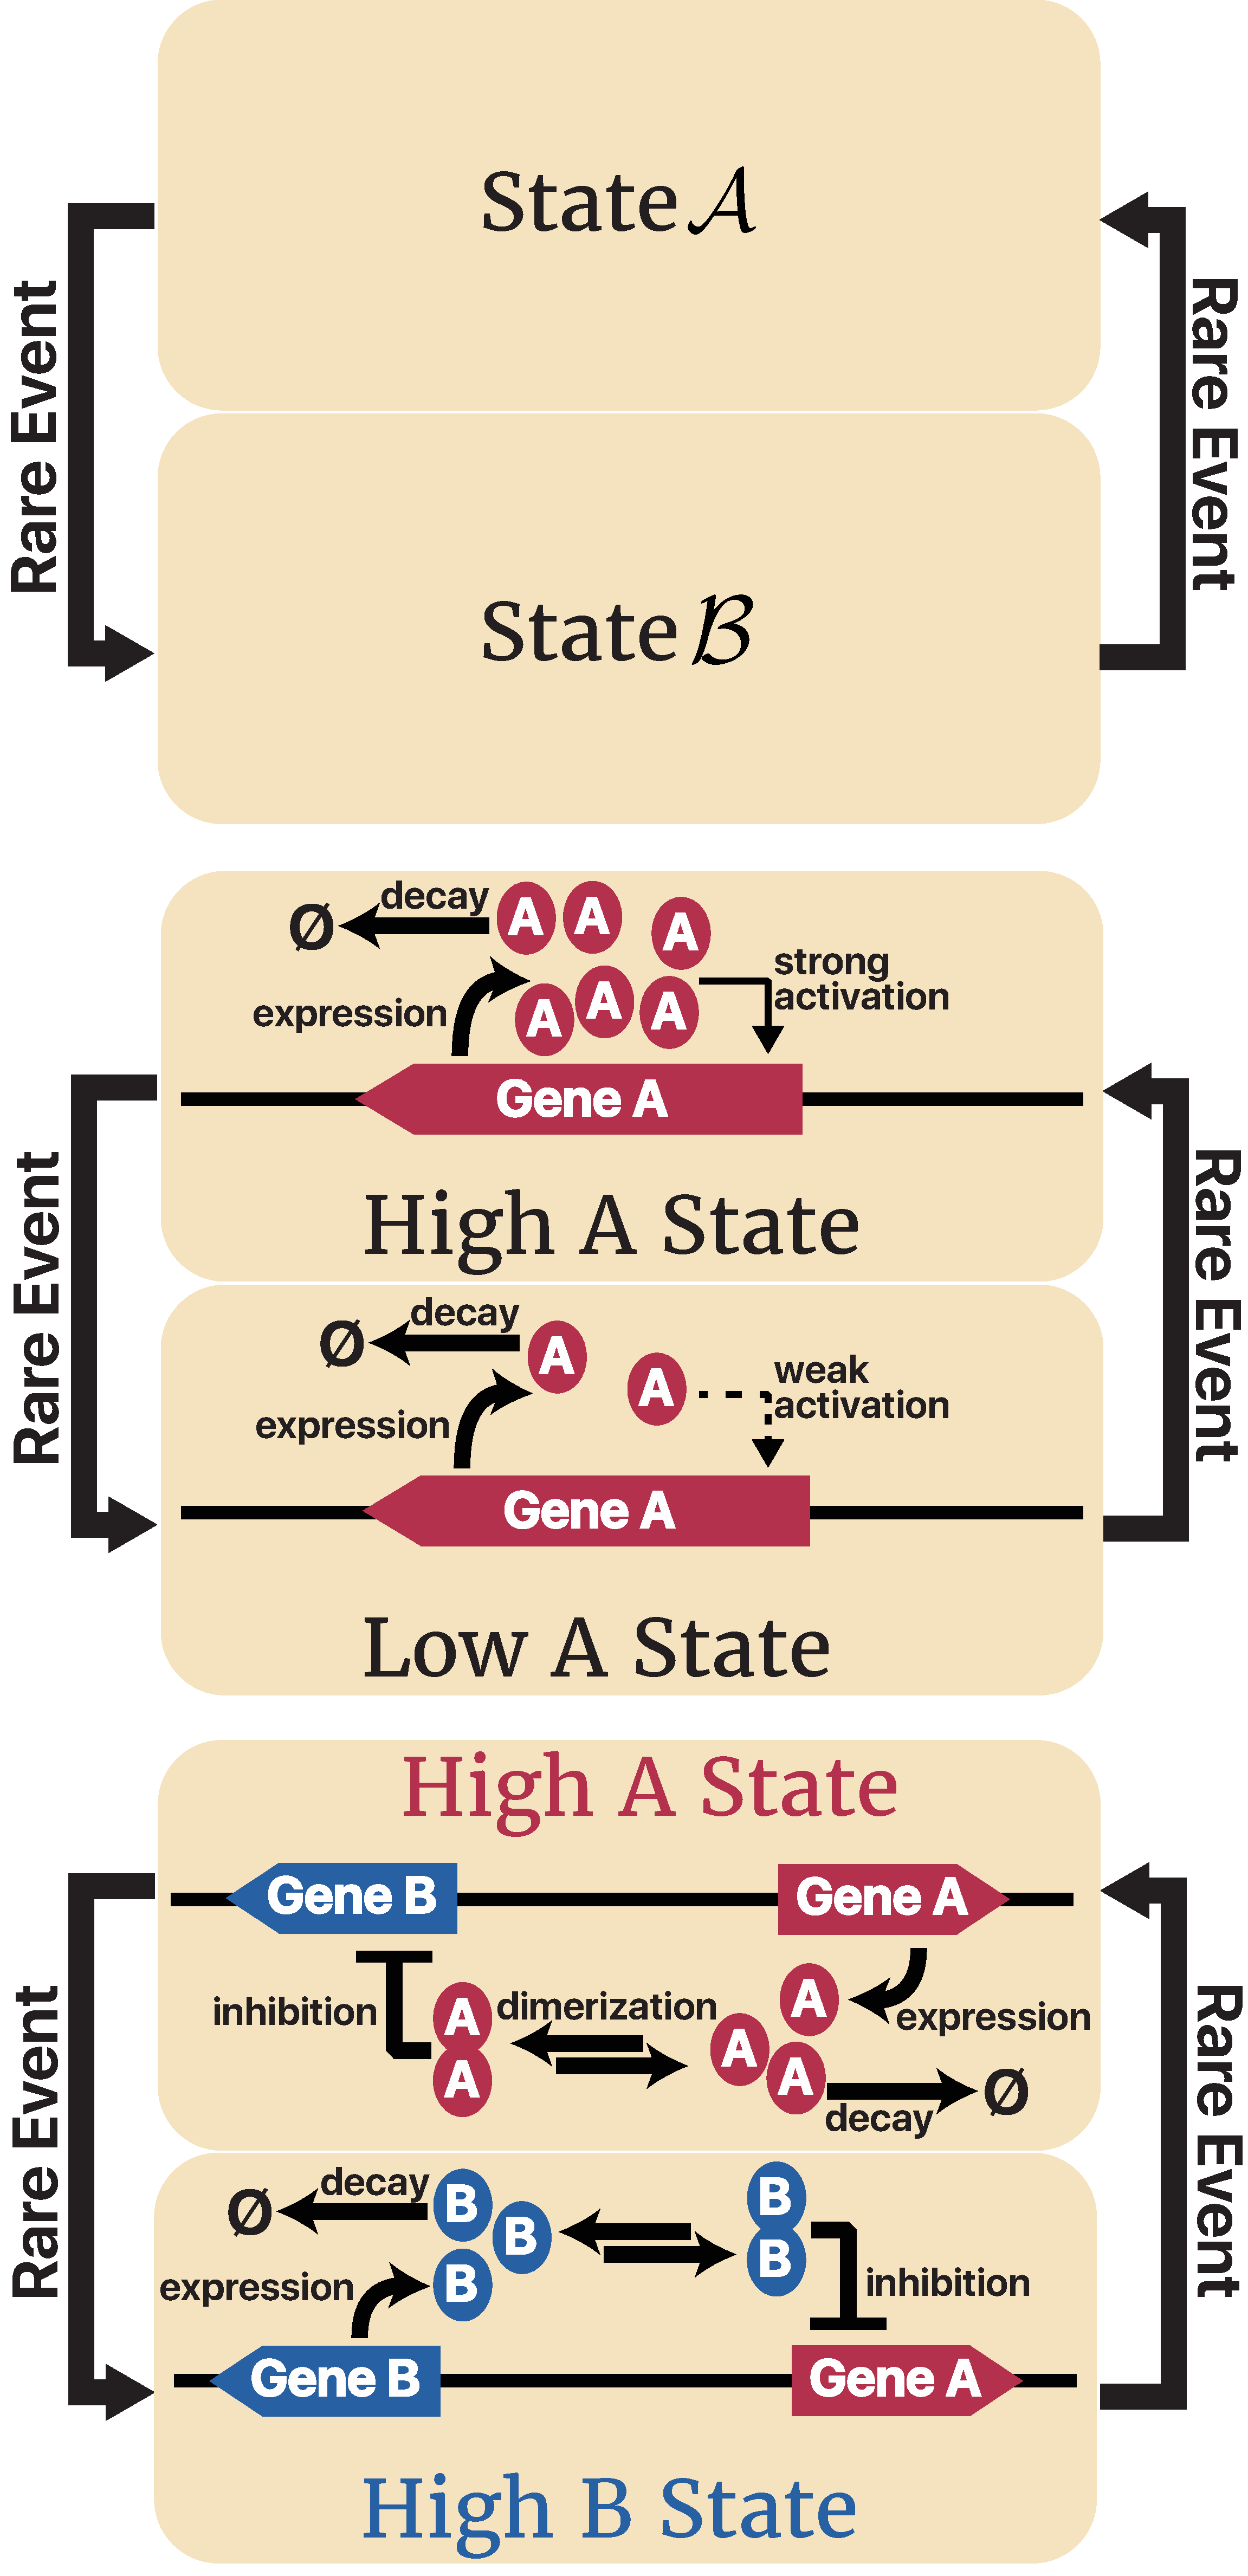
\includegraphics[width=8.45cm,height=\textheight,keepaspectratio]{{eces_chapter/model_schematics/schematic_composite_vertical}.pdf}
    \end{center}
%    \tracingmacros=1
    \caption{Schematics of the model systems investigated. \subplotcap{top} The \remname{} (\remabbrev{}, see \secref{sec:rem} and \tableref{tab:rem} for complete details). \subplotcap{middle} \srgname{} (\srgabbrev{}, see \secref{sec:srg} and \tablerefTwo{tab:srg_reactions}{tab:srg}). \subplotcap{bottom} \gtsname{} (\gtsabbrev{}, see \secref{sec:gts} and supplemental Table S1.}
%    \tracingmacros=0
    \label{fig:model_schematics}
\end{figure}
\clearpage
%\tracingmacros=0

%\begin{figure}[h]
%    \begin{center}
%        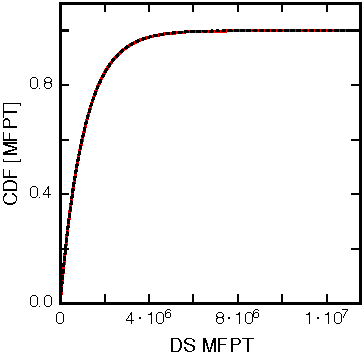
\includegraphics{{Figures/brute_force_mfpt_cdf}.pdf}
%    \end{center}
%    \caption{The empirical cumulative distribution function (shown in red) of $10^{5}$ first passage times gathered using \abr{DS}. The best fit exponential distribution, calculated using Maximum Likelihood Estimation, is shown as a black dotted line. The empirical CDF and the fitted exponential distribution appear to overlap almost exactly at the scale depicted in the above figure. All data was collected from simulations of the genetic toggle switch at $\theta=1.0$.}
%    \label{fig:brute_force_mfpt_cdf}
%\end{figure}
%\clearpage
%
%\begin{figure}[h]
%    \begin{center}
%        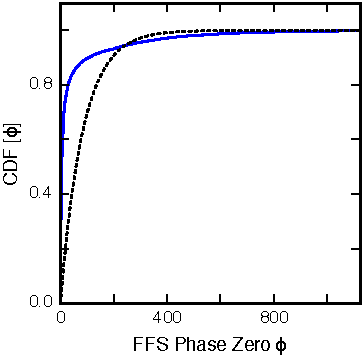
\includegraphics{{Figures/ffpilot_phase_zero_dwell_time_cdf}.pdf}
%    \end{center}
%    \caption{The empirical cumulative distribution function (shown in blue) of $10^{5}$ waiting times in between forward flux events during FFS phase 0. The best fit exponential distribution, calculated using Maximum Likelihood Estimation, is shown as a black dotted line. The moments of the empirical CDF and the best fit exponential distribution are not in good agreement. All data was collected from simulations of the genetic toggle switch at $\theta=1.0$.}
%    \label{fig:ffpilot_phase_zero_dwell_time_cdf}
%\end{figure}
%\clearpage

\begin{figure}[h]
    \begin{center}
        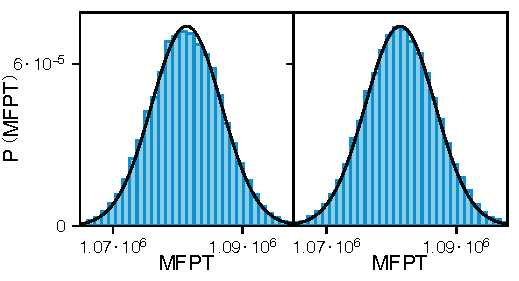
\includegraphics{{eces_chapter/Figures/toy_model_estimator_distributions_-_eg_1.0e-02_-_theta_1.0e+00_-_samples_1.6e5}.pdf}
    \end{center}
    \caption{\abr{MFPT} estimates for \abr{REM} calculated using (left) \abr{DS} and (right) \abr{FFPilot}. Shown are (blue bars) binned $\mfpttrue$ estimates from $1.6\cdot 10^5$ simulations with a 1\% error goal and (black lines) $\mfpttrue$ estimate distributions from \eqref{eq:fpt_clt_distribution} and \eqref{eq:PWest_asymptotic_dist}, respectively.}
    \label{fig:toy_model_estimator_distributions}
\end{figure}
\clearpage

\begin{figure}[h]
    \begin{center}
        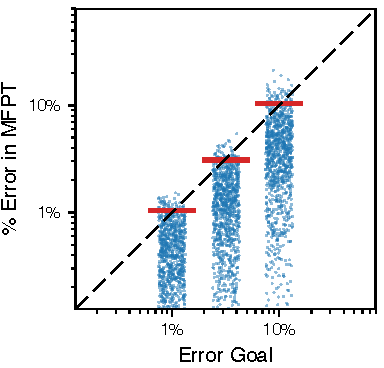
\includegraphics{{eces_chapter/Figures/toy_model_acutal_error_vs_predicted_error_-_cropped}.pdf}
    \end{center}
    \caption{Actual error vs error goal of \abr{FFPilot} simulations of the \abr{REM}. Each strip shows the \abr{MFPT} estimation error from (blue dots) 1000 independent \abr{FFPilot} simulations and (red lines) the 95th percentiles of the errors. Jitter was added to the x-position of the dots for visualization.}
    \label{fig:toy_model_actual_error_vs_predicted_error}
\end{figure}
\clearpage

%\begin{figure}[h]
%    \begin{center}
%        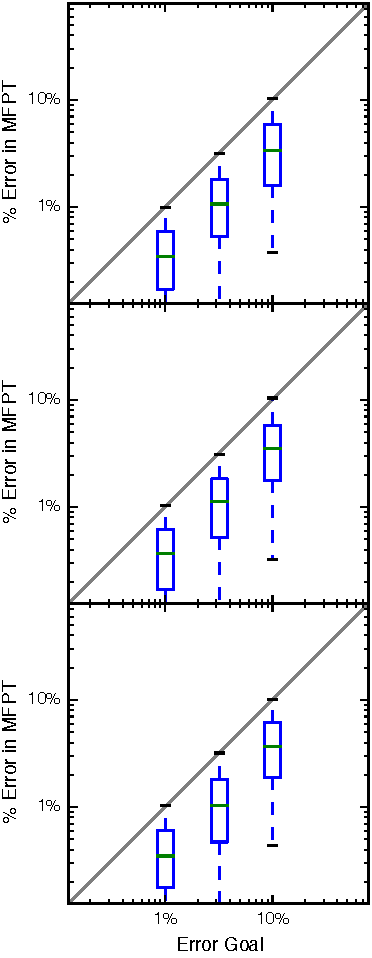
\includegraphics{{eces_chapter/Figures/toy_model_acutal_error_vs_predicted_error_-_boxplot}.pdf}
%    \end{center}
%    \caption{Box plots of actual error vs error goal for 9000 simulations of the simplified genetic toggle switch model. Each box is based on 1000 simulations run at the particular error goal corresponding to the position on the x axis. Each separate subplot is from a model with a different value of $\theta$ (from top to bottom, $\theta = 0.1, 1, 10$). All subplots are in log scale.}
%    \label{fig:toy_model_actual_error_vs_predicted_error_-_boxplot}
%\end{figure}
%\clearpage
%
%
%\begin{figure}[h]
%    \begin{center}
%        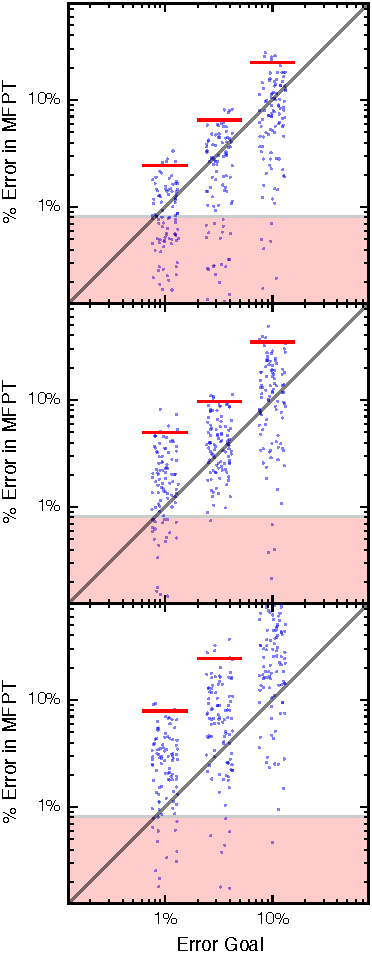
\includegraphics{{eces_chapter/Figures/cme_model_percent_error_vs_error_goal_-_reps_100}.pdf}
%    \end{center}
%    \caption{Results from 900 \abr{FFPilot} simulations. Specifically, strip plots showing a comparison of percent error vs error goal in estimated MFPT values from full CME simulations of different variants of the genetic toggle switch (from top to bottom, $\theta=0.1, 1, 10$). The 95th percentile of the error in the \abr{FFPilot} results at each of the different error goals is marked with a red line. Percent error was determined via a comparison of \abr{FFPilot} results with a highly accurate set of equivalent results produced using \abr{DS} ($10^5$ replicates). The 99\% confidence interval of the \abr{DS} comparison data set is marked as a red interval.}
%    \label{cme_model_percent_error_vs_error_goal}
%\end{figure}
%\clearpage
%
%
%\begin{figure}[h]
%    \begin{center}
%        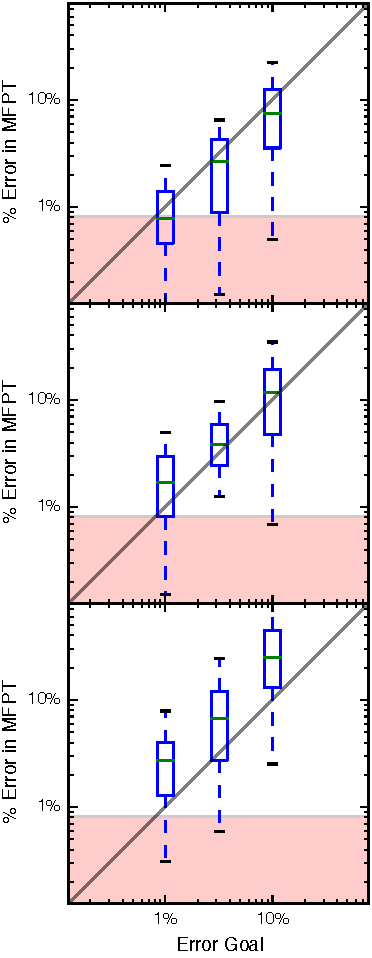
\includegraphics{{eces_chapter/Figures/cme_model_percent_error_vs_error_goal_-_reps_100_-_boxplot}.pdf}
%    \end{center}
%    \caption{Results from 900 \abr{FFPilot} simulations. Specifically, box and whisker plots showing a comparison of percent error vs error goal in estimated MFPT values from full CME simulations of different variants of the genetic toggle switch (from top to bottom, $\theta=0.1, 1, 10$). The green line marks the median of the distribution of errors at each different error goal, and the whiskers mark the 5th and 95th percentiles. Percent error was determined via a comparison of \abr{FFPilot} results with a highly accurate set of equivalent results produced using \abr{DS} ($10^5$ replicates). The 99\% confidence interval of the \abr{DS} comparison data set is marked as a red interval.}
%    \label{cme_model_percent_error_vs_error_goal_boxplot}
%\end{figure}
%\clearpage

\begin{figure}[h]
    \begin{center}
        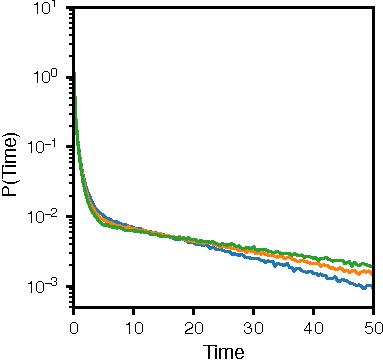
\includegraphics{{eces_chapter/Figures/name_srg_-_ffpilot_phase_zero_dwell_time_dist}.pdf}
    \end{center}
    \caption{Waiting times between forward crossing events during phase 0 of forward flux simulations of the \abr{SRG} models. Each line shows a distribution calculated from $10^6$ samples from a single phase 0 trajectory of (blue) $\SRGSLOWEST$, (orange) $\SRGSLOWER$ , and (green) $\SRGSLOW$.}
    \label{fig:name_srg_-_ffpilot_phase_zero_dwell_time_dist}
\end{figure}
\clearpage

\begin{figure}[h]
    \begin{center}
        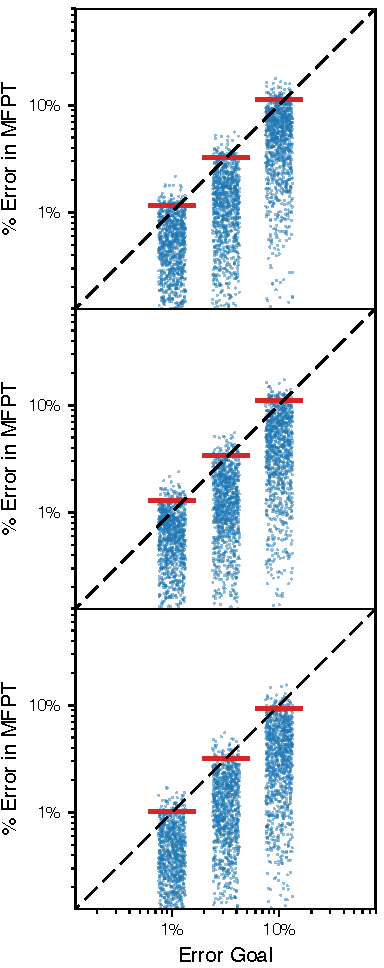
\includegraphics{{eces_chapter/Figures/name_h_-_stage_percent_error_-_error_goal_all_-_h_all}.pdf}
    \end{center}
    \caption{Actual error vs error goal of \abr{FFPilot} simulations for (top) $\SRGSLOWEST$, (middle) $\SRGSLOWER$, and (bottom) $\SRGSLOW$. Each strip shows (blue dots) 1000 independent \abr{FFPilot} simulations and (red lines) the 95th percentiles of the errors.}
    \label{fig:name_srg_-_error_goal_test_complete_-_h_all}
\end{figure}
\clearpage

\begin{figure}[h]
    \begin{center}
        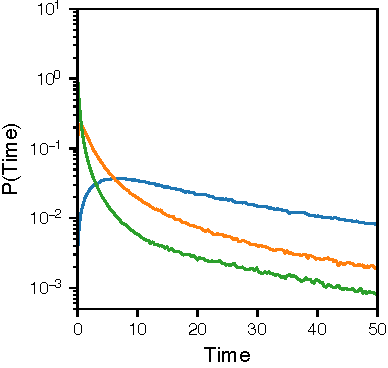
\includegraphics{{eces_chapter/Figures/name_gts_-_ffpilot_phase_zero_dwell_time_dist}.pdf}
    \end{center}
    \caption{Waiting times between forward crossing events during phase 0 of \abr{FFS} simulations of the \abr{GTS} models. Each line shows a distribution calculated from $10^6$ samples from a single phase 0 trajectory of (blue) $\GTSSLOWEST$, (orange) $\GTSSLOWER$, and (green) $\GTSSLOW$.}
    \label{fig:name_gts_-_ffpilot_phase_zero_dwell_time_dist}
\end{figure}
\clearpage

\begin{figure}[h]
    \begin{center}
        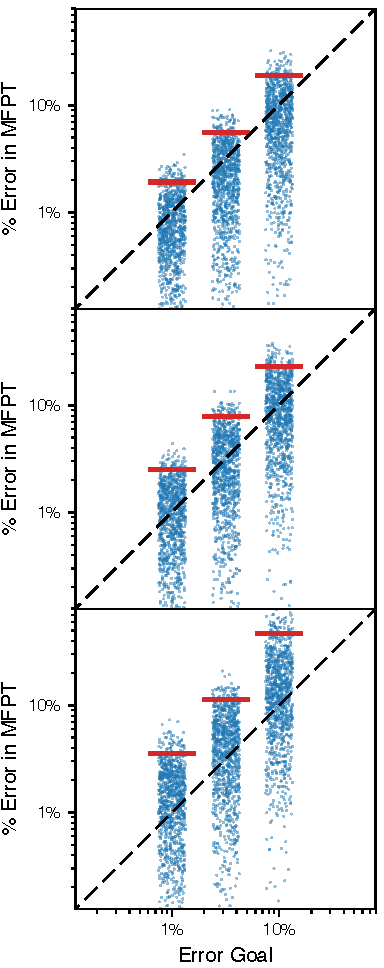
\includegraphics{{eces_chapter/Figures/name_theta_-_stage_percent_error_-_error_goal_all_-_theta_all}.pdf}
    \end{center}
    \caption{Actual error vs error goal of \abr{FFPilot} simulations for (top) $\GTSSLOWEST$, (middle) $\GTSSLOWER$, and (bottom) $\GTSSLOW$. Each strip shows (blue dots) 1000 independent \abr{FFPilot} simulations and (red lines) the 95th percentiles of the errors.}
    \label{fig:name_gts_-_error_goal_test_complete_-_theta_all}
\end{figure}
\clearpage

\begin{figure}[h]
    \begin{center}
        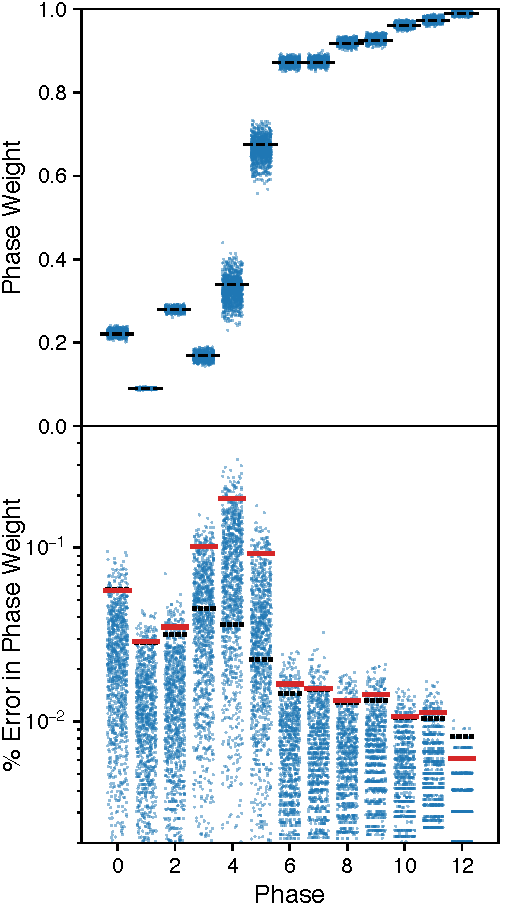
\includegraphics{{eces_chapter/Figures/name_theta_-_phase_weight_percent_error_-_error_goal_1.0e-01_-_theta_1.0e+01_enlarged}.pdf}
    \end{center}
    \caption{$\GTSSLOW$ phase weight estimates and errors. \subplotcap{top} The phase weights as estimated by (blue dots) 1000 independent \abr{FFPilot} simulations run to a 10\% error goal. The dashed black lines show the phase weights from an FFPilot simulation with a 0.1\% error goal. \subplotcap{bottom} The blue dots show the percent error of each phase weight estimate given in the top subplot, relative to the 0.1\% error goal simulation. Also shown are (red lines) the observed 95th error percentiles, and (dashed black lines) the expected 95th error percentiles.}
    \label{fig:name_gts_-_phase_weight_percent_error_-_error_goal_1.0e-01_-_theta_1.0e+01}
\end{figure}
\clearpage

\begin{figure}[h]
    \begin{center}
        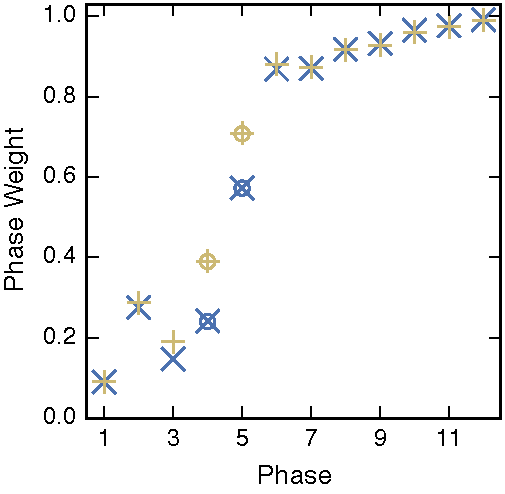
\includegraphics{{eces_chapter/Figures/name_gts_-_phase_weights_-_rep_6_8_-_theta_1.0e+01_-_enlarged}.pdf}
    \end{center}
    \caption{The phase weights of two replicates: (blue x) Replicate 6 and (gold +) Replicate 8, from a $\GTSSLOW$ \abr{FFPilot} simulation run to an error goal of 10\%. Circles show weights for phases 4 and 5 calculated via an alternative method using \eqref{eq:reconstituted_phase_weights}.}
    
    %The phase weights of phases 4 and 5 were recalculated using an alternative method that only used the landscapes assembled by the replicates, rather than the outcomes of the simulations in the given phase. These recalculated phase weights are shown as hollow circles (Replicate 6 in blue, Replicate 8 in gold).}
%    \caption{The phase weights of two replicates, Replicate 6 \inlinelegend{{eces_chapter/Figures/name_gts_-_phase_weights_-_rep_6_8_-_theta_1.0e+01_marker_0}.pdf} and Replicate 8 \inlinelegend{{eces_chapter/Figures/name_gts_-_phase_weights_-_rep_6_8_-_theta_1.0e+01_marker_1}.pdf}, of an \abr{FFPilot} simulation of the genetic toggle switch (with $\theta=10$) run to an error goal of 10\%. In phases 4 and 5, which are the two phases leading up to the midpoint of the transition path, the phase weights of these two replicates diverge greatly. The phase weights of phases 4 and 5 were recalculated using an alternative method that only used the landscapes assembled by the replicates, rather than the outcomes of the simulations in the given phase. These recalculated phase weights are shown as hollow circles (Replicate 6 \inlinelegend{{eces_chapter/Figures/name_gts_-_phase_weights_-_rep_6_8_-_theta_1.0e+01_marker_2}.pdf}, Replicate 8 \inlinelegend{{eces_chapter/Figures/name_gts_-_phase_weights_-_rep_6_8_-_theta_1.0e+01_marker_3}.pdf}}).
    \label{fig:name_gts_-_phase_weights_-_rep_6_8_-_theta_1.0e+01}
\end{figure}
\clearpage

\begin{figure}[h]
    \begin{center}
        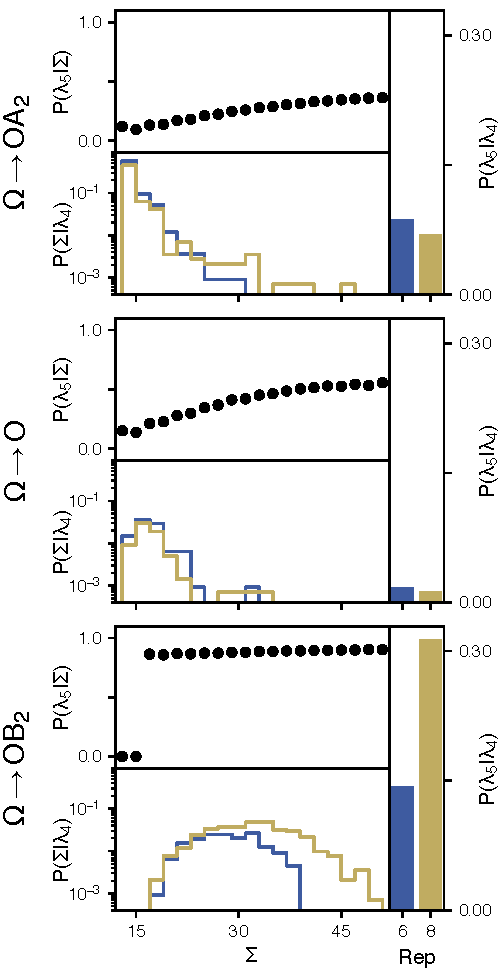
\includegraphics{{eces_chapter/Figures/name_gts_-_phase_weight_4_split_by_operator_-_rep_6_8_-_theta_1.0e+01_-_dists_-_one-col}.pdf}
%        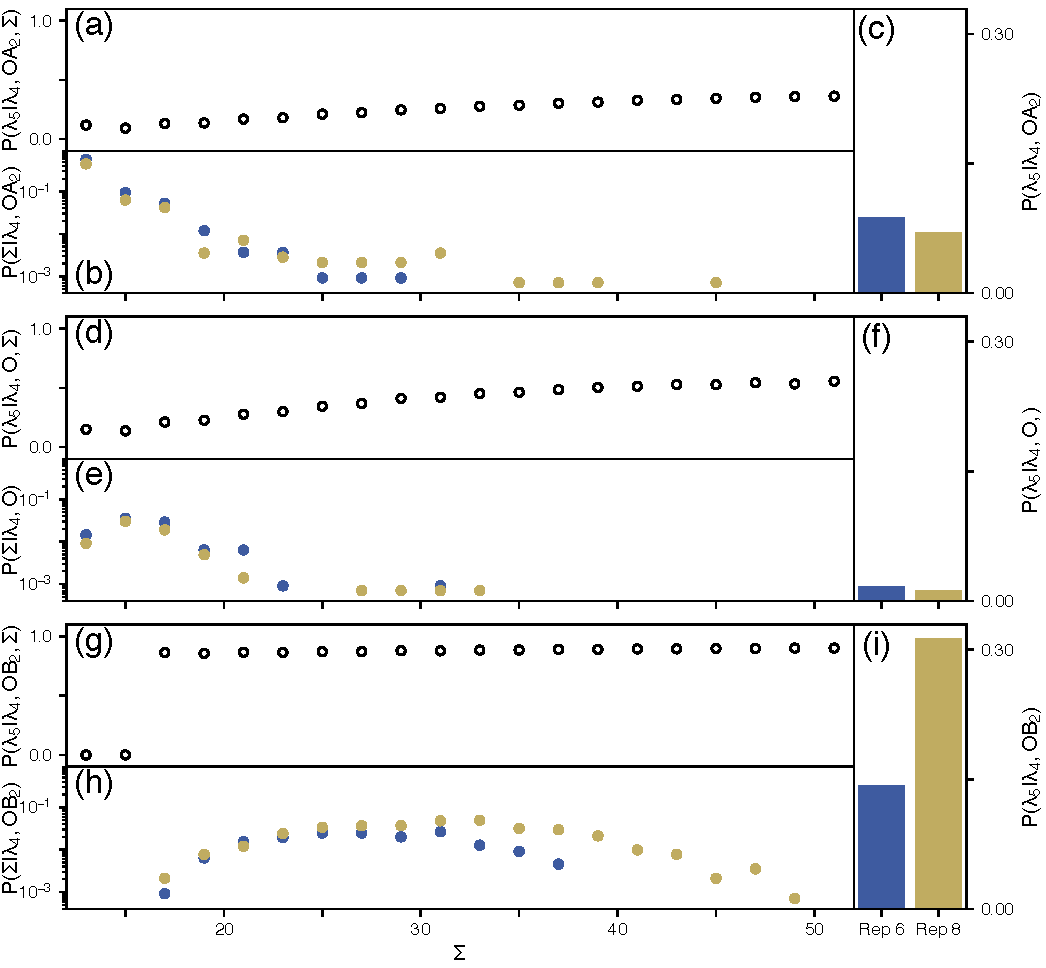
\includegraphics{{eces_chapter/Figures/name_gts_-_phase_weight_4_split_by_operator_-_rep_6_8_-_theta_1.0e+01_-_dots}.pdf}
%        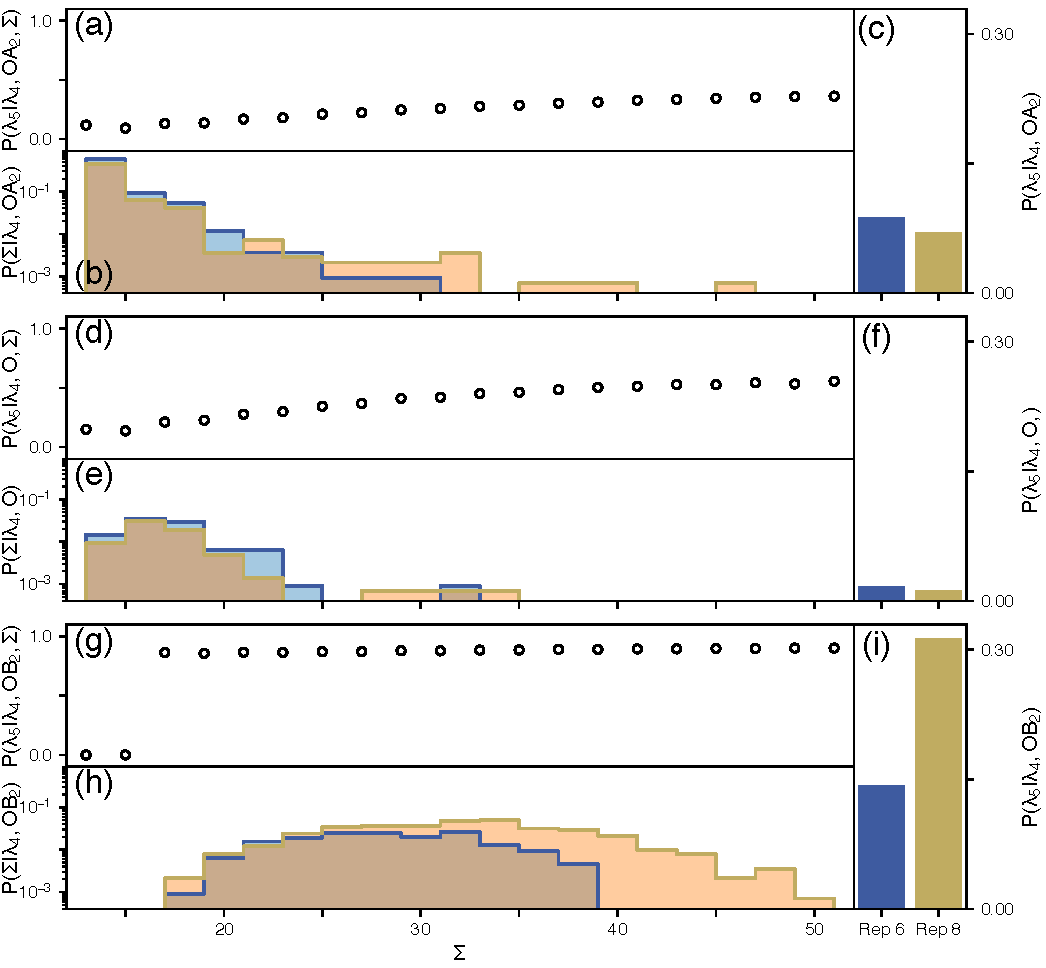
\includegraphics{{eces_chapter/Figures/name_gts_-_phase_weight_4_split_by_operator_-_rep_6_8_-_theta_1.0e+01_-_dists_filled}.pdf}
    \end{center}
    \caption{Breakout of the calculation of phase weight 5 for replicates 6 and 8. Each group of three plots show data from a slice of \abr{GTS} state space with a different $\gtsostate$, the state of the operator DNA. Each subplot within a group shows different probability data. (dots) The probability of a trajectory launched from a point on $\ifacex{4}$ fluxing forward to $\ifacex{5}$ vs the orthogonal order parameter $\gtsbpa$. (lines) The occupancy along $\gtsbpa$ at interface $\ifacex{4}$ for (blue) replicate 6 and (gold) replicate 8. (bars) The cumulative probability of fluxing forward across $\ifacex{5}$ when starting at the specified $\gtsostate$ for (blue) replicate 6 and (gold) replicate 8.}
    \label{fig:name_gts_-_phase_weight_4_split_by_operator_-_rep_6_8_-_theta_1.0e+01}
\end{figure}
\clearpage

%\begin{figure}[h]
%    \begin{center}
%        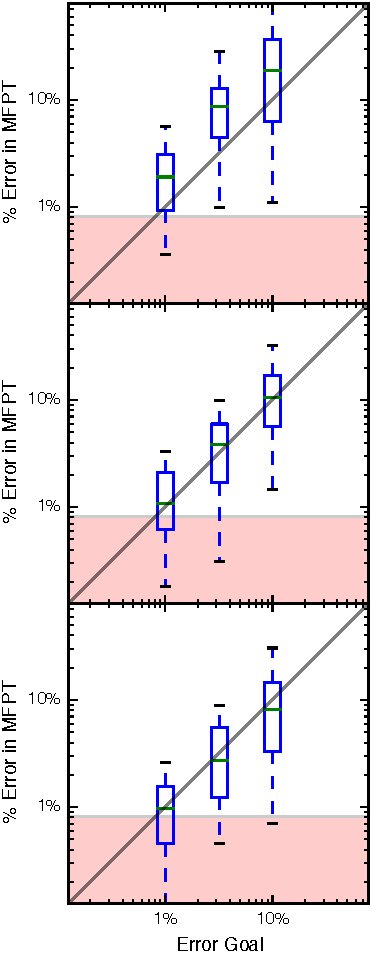
\includegraphics{{eces_chapter/Figures/cme_model_percent_error_vs_error_goal_at_different_phase_zero_mults-_reps_100_-_theta_1.0e+01_-_boxplot}.pdf}
%    \end{center}
%    \caption{Box and whisker plots showing the effect of oversampling during \abr{FFPilot} phase 0 on overall simulation accuracy. From top to bottom, the subplots show the results from 300 \abr{FFPilot} simulations (100 per error goal) of the genetic toggle switch at $\theta=10$ carried out with 1X, 10X, and 100X sampling during \abr{FFPilot} phase 0. The calculation of the percent error in the estimated MFPT was carried out with the same protocol as described in the caption of fig \ref{cme_model_percent_error_vs_error_goal_boxplot}. }
%    \label{fig:cme_model_percent_error_vs_error_goal_at_different_phase_zero_mults}
%\end{figure}
%\clearpage
%
%\begin{figure}[h]
%    \begin{center}
%        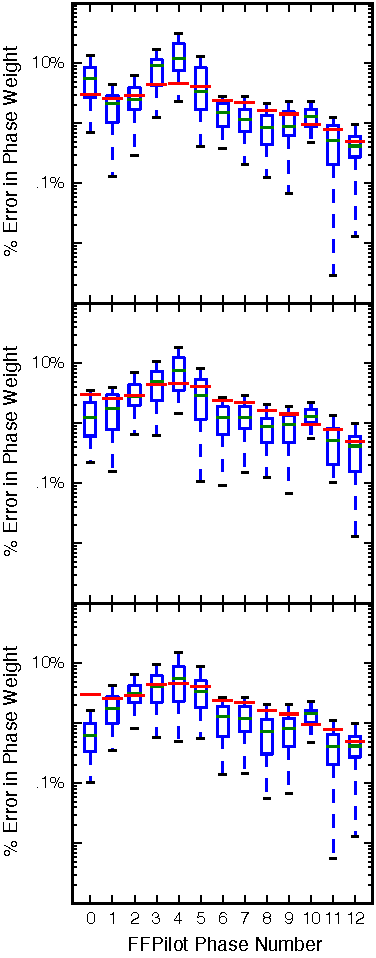
\includegraphics{{eces_chapter/Figures/ffpilot_phase_weight_percent_errors_vs_predicted_errors_-_theta_1.0e+01}.pdf}
%    \end{center}
%    \caption{Box and whisker plots showing an in-depth examination of how the errors in each of the phase weights change as more samples are taken during \abr{FFPilot} phase 0. From top to bottom, 1X, 10X, and 100X sampling during \abr{FFPilot} phase 0 was performed.   Each subplot contains data from 100 \abr{FFPilot} simulation of the genetic toggle switch at $\theta=10$ carried out with an error goal of $10\%$. \newline
%    The red lines show the predicted value for the 95th percentile of each of the phase weight error distributions. In other words, the optimizing equation predicts that the top whisker of each box will be bellow the red line, and further that if this condition is met it is likely that the error in the MFPT will also be in the desired range. However, the optimizing equation does not take the effects of landscape error directly into account.}
%    \label{fig:ffpilot_phase_weight_percent_errors_vs_predicted_errors}
%\end{figure}
%\clearpage

\begin{figure}[h]
    \begin{center}
        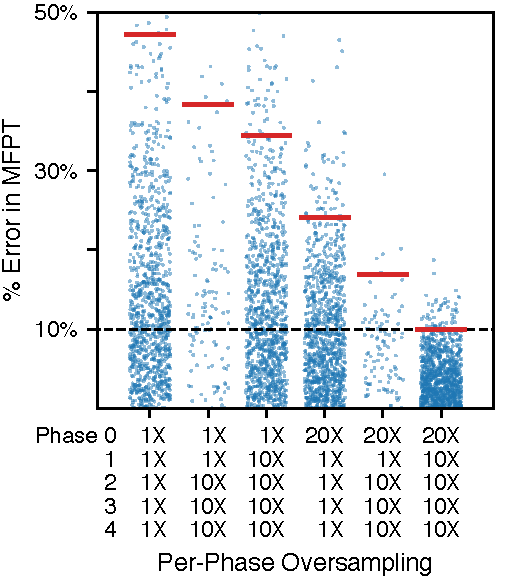
\includegraphics{{eces_chapter/Figures/name_gts_-_stage_fpt_percent_error_-_landscape_fudge_several_-_error_goal_1.0e-01_-_theta_1.0e+01_-_enlarged}.pdf}
    \end{center}
    \caption{Errors from simulations executed with various oversampling schemes. The extent of oversampling in each phase for the separate schemes is indicated beneath each column of results. All simulations were of $\GTSSLOW$ run to an error goal of 10\%. Red lines show the 95th error percentiles.}
    \label{fig:name_gts_-_stage_fpt_percent_error_-_landscape_fudge_several_-_error_goal_1.0e-01_-_theta_1.0e+01}
\end{figure}
\clearpage

\begin{figure}[h]
    \begin{center}
        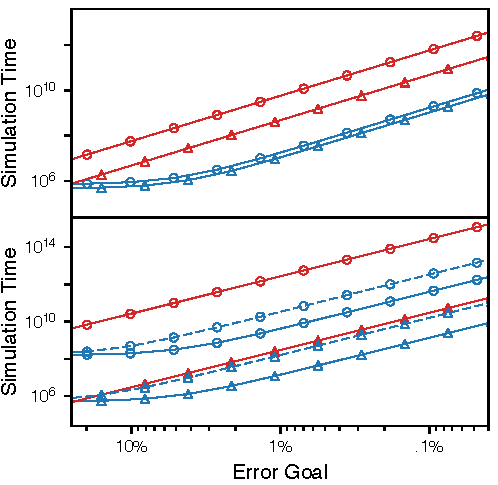
\includegraphics{{eces_chapter/Figures/name_theta_-_name_h_-_speedup_plot_-_simtime_vs_error_goal}.pdf}
    \end{center}
    \caption{Simulation time vs error goal for several \abr{SRG} and \abr{GTS} models. Simulation time was calculated using \eqref{eq:ds_cost} for (red lines) \abr{DS}, and \eqref{eq:ffpilot_cost} for (blue lines) \abr{FFPilot} and (dashed line) \abr{FFPilot} with oversampling to correct the landscape error. Parameters were taken from \tablerefTwo{tab:srg}{tab:gts}. (top) Data from (circles) $\SRGSLOWEST$ and (triangles) $\SRGSLOW$. (bottom) Data from (circles) $\GTSSLOWEST$ and (triangles) $\GTSSLOW$.}
    \label{fig:name_srg_-_speedup_plot_-_simtime_vs_moe}
\end{figure}
\clearpage

\begin{figure}[h]
    \begin{center}
        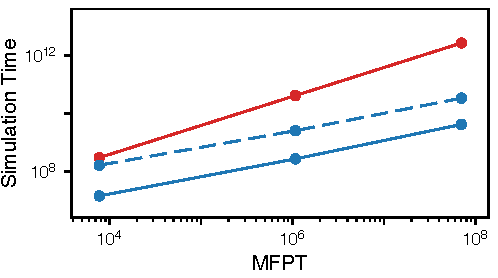
\includegraphics{{eces_chapter/Figures/name_theta_-_speedup_plot_-_simtime_vs_mfpt_-_error_goal_1.0e-02}.pdf}
    \end{center}
    \caption{Simulation time vs \abr{MFPT} for several \abr{GTS} models. Simulation times are shown for (red dots) \abr{DS}, (blue dots) \abr{FFPilot}, and (blue dots with dashed line) \abr{FFPilot} with oversampling to correct for landscape error. The simulation times shown are averaged across 1000 simulations. Connecting lines added for illustration.}
    \label{fig:name_theta_-_speedup_plot_-_simtime_vs_mfpt_-_error_goal_1.0e-02}
\end{figure}
\clearpage

%\begin{figure}[h]
%    \begin{center}
%        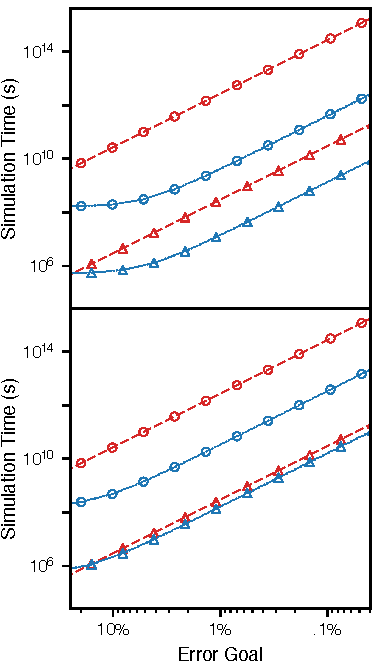
\includegraphics{{eces_chapter/Figures/name_theta_-_speedup_plot_-_simtime_vs_error_goal}.pdf}
%    \end{center}
%    \caption{A comparison of how the simulation time scales with respect to error goal for the genetic toggle switch models $\GTSSLOW$ (triangles) and $\GTSSLOWEST$ (circles). The simulation time for both \abr{DS} (red lines) and \abr{FFPilot} Sampling (blue lines) are shown. The results were derived from \eqrefTwo{eq:ds_sim_time}{eq:ffpilot_cost}. The equation was parameterized from the mean results of 1000 simulations of each model run at a 1\% error goal. The results without any correction for landscape error are shown in the top subplot, and the results with the landscape corrections determined in \secref{sec:oversampling} are shown in the bottom subplot.}
%    \label{fig:name_theta_-_speedup_plot_-_simtime_vs_error_goal}
%\end{figure}
%\clearpage
%
%\begin{figure}[h]
%    \begin{center}
%        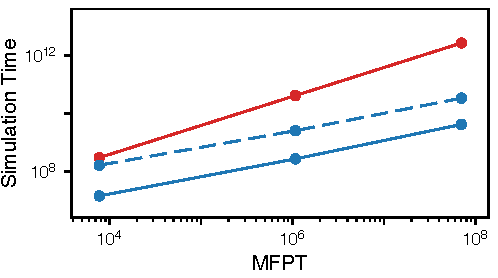
\includegraphics{{eces_chapter/Figures/name_theta_-_speedup_plot_-_simtime_vs_mfpt_-_error_goal_1.0e-02}.pdf}
%    \end{center}
%    \caption{A comparison of how the simulation time required for \abr{DS} (red circles) and \abr{FFPilot} Sampling (blue circles) scale with respect to the \abr{MFPT} of the various versions of the \gtsname{}. The rate at which a given version of the \gtsname{} transitions from state to state can be tuned using the relative protein churn rate parameter $\theta$. The results were derived from \eqref{eq:optimizing_equation_general_form}. The equation was parameterized from empirical results drawn from 1000 \abr{FFPilot} simulations of the \gtsname{} models run at a $\%1$ error goal.}
%    \label{fig:name_theta_-_speedup_plot_-_simtime_vs_mfpt_-_error_goal_1.0e-02}
%\end{figure}
%\clearpage
%
%
%\begin{figure}[h]
%    \begin{center}
%        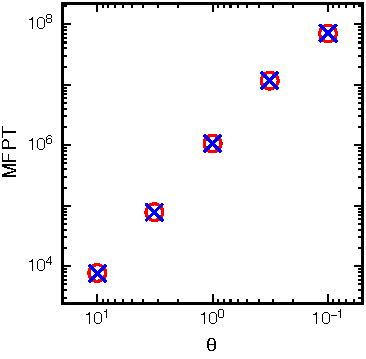
\includegraphics{{eces_chapter/Figures/ffpilot_bf_mfpt_vs_theta_scatter_-_eg_1.0e-02}.pdf}
%    \end{center}
%    \caption{Comparison of \abr{MFPT} values calculated with \abr{DS} and with \abr{FFPilot}. Both methods were run with a $1\%$ error goal, and the \abr{FFPilot} simulations were run with 10X phase 0 sampling. Each data point is the average of 5 simulations, and error bars are not shown because they are too small to see.}
%    \label{fig:mfpt_vs_theta}
%\end{figure}
%\clearpage
%
%\begin{figure}[h]
%    \begin{center}
%        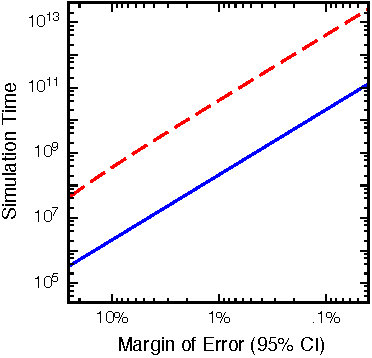
\includegraphics{{eces_chapter/Figures/toy_model_simulation_time_scaling_with_percent_error}.pdf}
%    \end{center}
%    \caption{A comparison of how the simulation time required for \abr{DS} (red dashed line) and \abr{FFPilot} Sampling (blue line) scale with respect to error goal. The results were derived from \eqref{eq:optimizing_equation_general_form}. The equation was parameterized from empirical results drawn from simulations of the full CME model of the genetic toggle switch. The parameters for each individual data point were generated from the average fit of the results of 5 simulations run at a $\%1$ error goal.}
%    \label{fig:toy_model_simulation_time_scaling_with_percent_error}
%\end{figure}
%\clearpage
%
%\begin{figure}[h]
%    \begin{center}
%        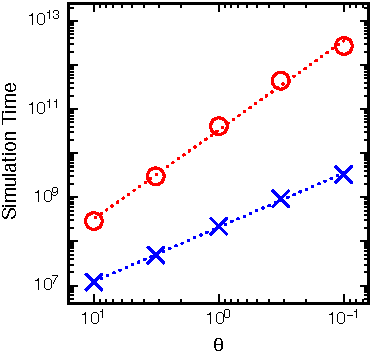
\includegraphics{{eces_chapter/Figures/ffpilot_bf_simulation_time_vs_theta_scatter}.pdf}
%    \end{center}
%    \caption{A comparison of how the simulation time required for \abr{DS} (red circles) and \abr{FFPilot} Sampling (blue Xs) scale with respect to the relative protein churn rate parameter $\theta$. Power law fits to the data are shown as dotted lines. Smaller values of $\theta$ result in a version of the genetic toggle switch that transitions more slowly from state to state, whereas larger values of $\theta$ cause it transition more frequently. The results were derived from \eqref{eq:optimizing_equation_general_form}. The equation was parameterized from empirical results drawn from simulations of the full CME model of the genetic toggle switch. The parameters for each individual data point were generated from the average fit of the results of 5 simulations run at a $\%1$ error goal.}
%    \label{fig:simulation_time_vs_theta}
%\end{figure}
%\clearpage
%
%\begin{figure}[h]
%    \begin{center}
%        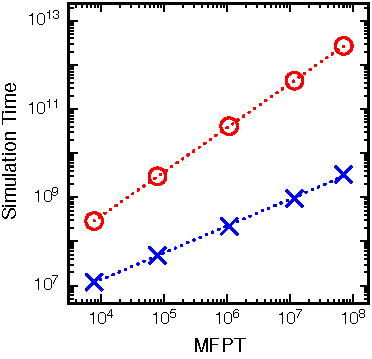
\includegraphics{{eces_chapter/Figures/ffpilot_bf_simulation_time_vs_mfpt_scatter}.pdf}
%    \end{center}
%    \caption{A comparison of how the simulation time required for \abr{DS} (red circles) and \abr{FFPilot} Sampling (blue Xs) scale with respect to the \abr{MFPT} of the various versions of the genetic toggle switch. Power law fits to the data are shown as dotted lines. The rate at which a given version of the genetic toggle switch transitions from state to state can be tuned using the relative protein churn rate parameter $\theta$. The results were derived from \eqref{eq:optimizing_equation_general_form}. The equation was parameterized from empirical results drawn from simulations of the full CME model of the genetic toggle switch. The parameters for each individual data point were generated from the average fit of the results of 5 simulations run at a $\%1$ error goal.}
%    \label{fig:simulation_time_vs_mfpt}
%\end{figure}
%\clearpage


%\input{error_control_of_enhanced_sampling-figures_roundfile}

%\end{document}

%% cut down version of supplemental main .tex file for including references

%\documentclass[class=article, float=false, crop=false]{standalone}
%\documentclass[10pt,letterpaper]{article}
%
%\input{error_control_of_enhanced_sampling-header}
%
%\begin{document}

\beginsupplemental

\subsection{Alternative derivation of variance of the $\mfpttrue$ estimator}
\label{sec:sup_alt_var}
Instead of using the delta method as in \secref{sec:phase_weight_moments} of the main paper, the variance of the \abr{FFS} $\mfpttrue$ estimator can also be derived from the fundamental properties of variance (though no explicit information about the underlying distribution of $\mfptest$ is gained this way). From the general properties of variance it is known that for independent random variables $X_0, X_1, ..., X_i$:
        \begin{equation}
        \label{eq:product_variance_compact}
            \V{\prod_i X_i} = \prod_i \left(\V{X_i} + \E{X_i}^2\right) - \prod_i \E{X_i}^2.
        \end{equation}
The righthand side of the above \eqref{eq:product_variance_compact} can be rewritten in terms of a generalized variance $\gvarsymb$\supercite{Goodman:1962uc}:
        \begin{equation}
        \label{eq:product_variance_gvar_grouped}
            \V{\prod_i X_i} = \prod_i \E{X_i}^2 \left( \sum_i \GVAR{X_i} + \sum_{i_0 < i_1} \GVAR{X_{i_0}} \GVAR{X_{i_1}} + \sum_{i_0 < i_1 < i_2} \GVAR{X_{i_0}} \GVAR{X_{i_1}} \GVAR{X_{i_2}} + \cdots, \right)
        \end{equation}
where $\GVAR{X} = \frac{\V{X}}{\E{X}^2}$. If the expected values are much larger than the variances, the higher order terms of $\V{\prod_i X_i}$ can be ignored without a large loss of accuracy. The condition:
    \begin{equation}
    \label{eq:product_variance_approx_condition}
        \E{X_i} >> \V{X_i} \quad \forall X_i,
    \end{equation}
implies that:
    \begin{align*}
        \GVAR{X_{i_0}} &>> \GVAR{X_{i_0}}\GVAR{X_{i_1}} &\quad &\forall X_{i_0}, X_{i_1}, \\
        \GVAR{X_{i_0}} &>> \GVAR{X_{i_0}}\GVAR{X_{i_1}}\GVAR{X_{i_2}} &\quad &\forall X_{i_0}, X_{i_1}, X_{i_2},\\
        \vdots
    \end{align*}
This regime yields an easy to work with approximation of \eqref{eq:product_variance_gvar_grouped} as a series of of independent terms that only depend on a single $X_i$:
    \begin{equation}
    \label{eq:product_variance_approx}
        \V{\prod_i X_i} \approx \prod_i \E{X_i}^2 \sum_i \GVAR{X_i}.
    \end{equation}

Each \abr{FFS} simulation phase $\phase$ can be conceptualized as taking a series of samples from a random variable $\phrv$ (see \secref{sec:ds_es_description} in the main paper). The phase weight estimator $\pwest$ is then the mean of the $\phrv$ samples. The moments of each $\pwest$ can be derived using the standard expected value and variance identities\supercite{Borovkov:2013hf}, giving:
    \begin{align}
    \label{eq:pwest_moments_alternative}
        \begin{split}
            \E{\pwest} &= \pwtrue, \\
            \V{\pwest} &= \frac{\V{\phrv}}{n_i}.
        \end{split}
    \end{align}
Since $\V{w_i}$ is a fixed value, the value of each $\V{\pwest}$ term trends monotonically downward as $\samplecount$ increases. If $n_i$ is assumed to be set to a large value, then it is reasonable to assume that $\E{\pwest} >> \V{\pwest}$ as well. In this regime the condition in \eqref{eq:product_variance_approx_condition} is satisfied, and so we can apply the simplified formula for the product variance to the phase weights. Plugging the moments in \eqref{eq:pwest_moments_alternative} into \eqref{eq:product_variance_approx} yields:
    \begin{equation*}
        \V{\mfptest} = \V{\prod_\phase \pwest} \approx \prod_i \E{\pwest}^2 \sum_i \frac{\GVAR{\pwest}}{n_i} = \prod_j \pwtruesqx{j} \sum_i \frac{\V{\phrv}}{\pwtruesq n_i}.
    \end{equation*}
    
%$\phrvx{0}$ draws from the distribution of waiting times in between forward flux events across $\ifacex{0}$, whereas $\phrvx{i>0}$ draws from the distribution of trajectory outcomes (\ie 0 for trajectories that fall back, 1 for trajectories that flux forward).

%and so
%        \begin{equation*}
%            \V{\PWest} = \prod_i \E{\pwest}^2 \left( \sum_i \GVAR{\pwest} + \sum_{i_0 < i_1} \GVAR{\pwestx{i_0}} \GVAR{\pwestx{i_1}} + \cdots \right)
%        \end{equation*}

\continuesupplemental

\subsection{Speedup equation misc}
We present here the complete FFPilot equation for the speedup of FFPilot over DS simulation, $\frac{\Costds}{\Costffpilot}$, without the high simulation accuracy/low error goal approximation used in the main paper:
    \begin{equation*}
        \frac{\Costds}{\Costffpilot} = \mfpttrue /\left( \left(\sum _{\phase=1}^\Phase \sqrt{\frac{\pctrue \left( 1-\probphase \right)}{\probphase}}+\sqrt{\frac{\pctruex{0} \pwvtrueshortx{0}}{w_0^2}}\right)^2 + n_{pilot} \frac{\moesq}{\zscoresq} \left( \pctruex{0} + \sum _{j=1}^N \frac{\pctruex{j}}{p_j} \right) \right).
	\end{equation*}

%\documentclass[class=article, float=false, crop=false]{standalone}
%\documentclass[10pt,letterpaper]{article}
%
%\input{error_control_of_enhanced_sampling-header}
%
%\begin{document}

\continuesupplemental

\subsection{Supplemental figures}
\label{sec:supplemental_figures}

\begin{figure}[h]
    \begin{center}
    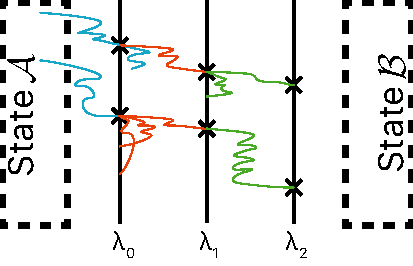
\includegraphics{{model_schematics/ffpilot_pilot_stage_-_fixed}.pdf}
    \end{center}
    \caption[Schematic example of a pilot stage from a FFPilot simulation]{Schematic example of a pilot stage from a FFPilot simulation, with total phase count $\Phase = 3$ and $\samplecountpilot = 2$. Trajectories from phases (blue) 0, (red) 1, and (green) 2 shown in different colors.}
    \label{fig:ffpilot_pilot_stage}
\end{figure}
\clearpage

\begin{figure}[h]
    \begin{center}
        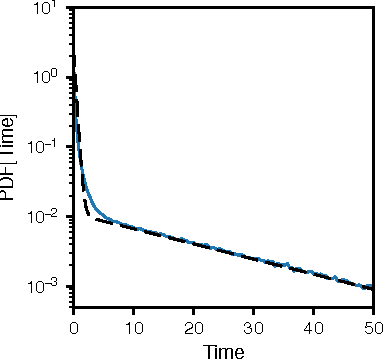
\includegraphics{{supplemental/figures/name_srg_-_ffpilot_phase_zero_dwell_time_dist_-_with_fit_-_fixed}.pdf}
    \end{center}
    \caption[Distribution of times in between events during phase 0 of forward flux simulation of $\SRGSLOW$]{Distribution of waiting times in between phase 0 forward flux events for $\SRGSLOW$, $10^6$ samples. Dashed line is a fit of a mixture of two exponential distributions.}
    \label{fig:name_srg_-_ffpilot_phase_zero_dwell_time_dist_-_with_fit}
\end{figure}
\clearpage

\begin{figure}[h]
    \begin{center}
        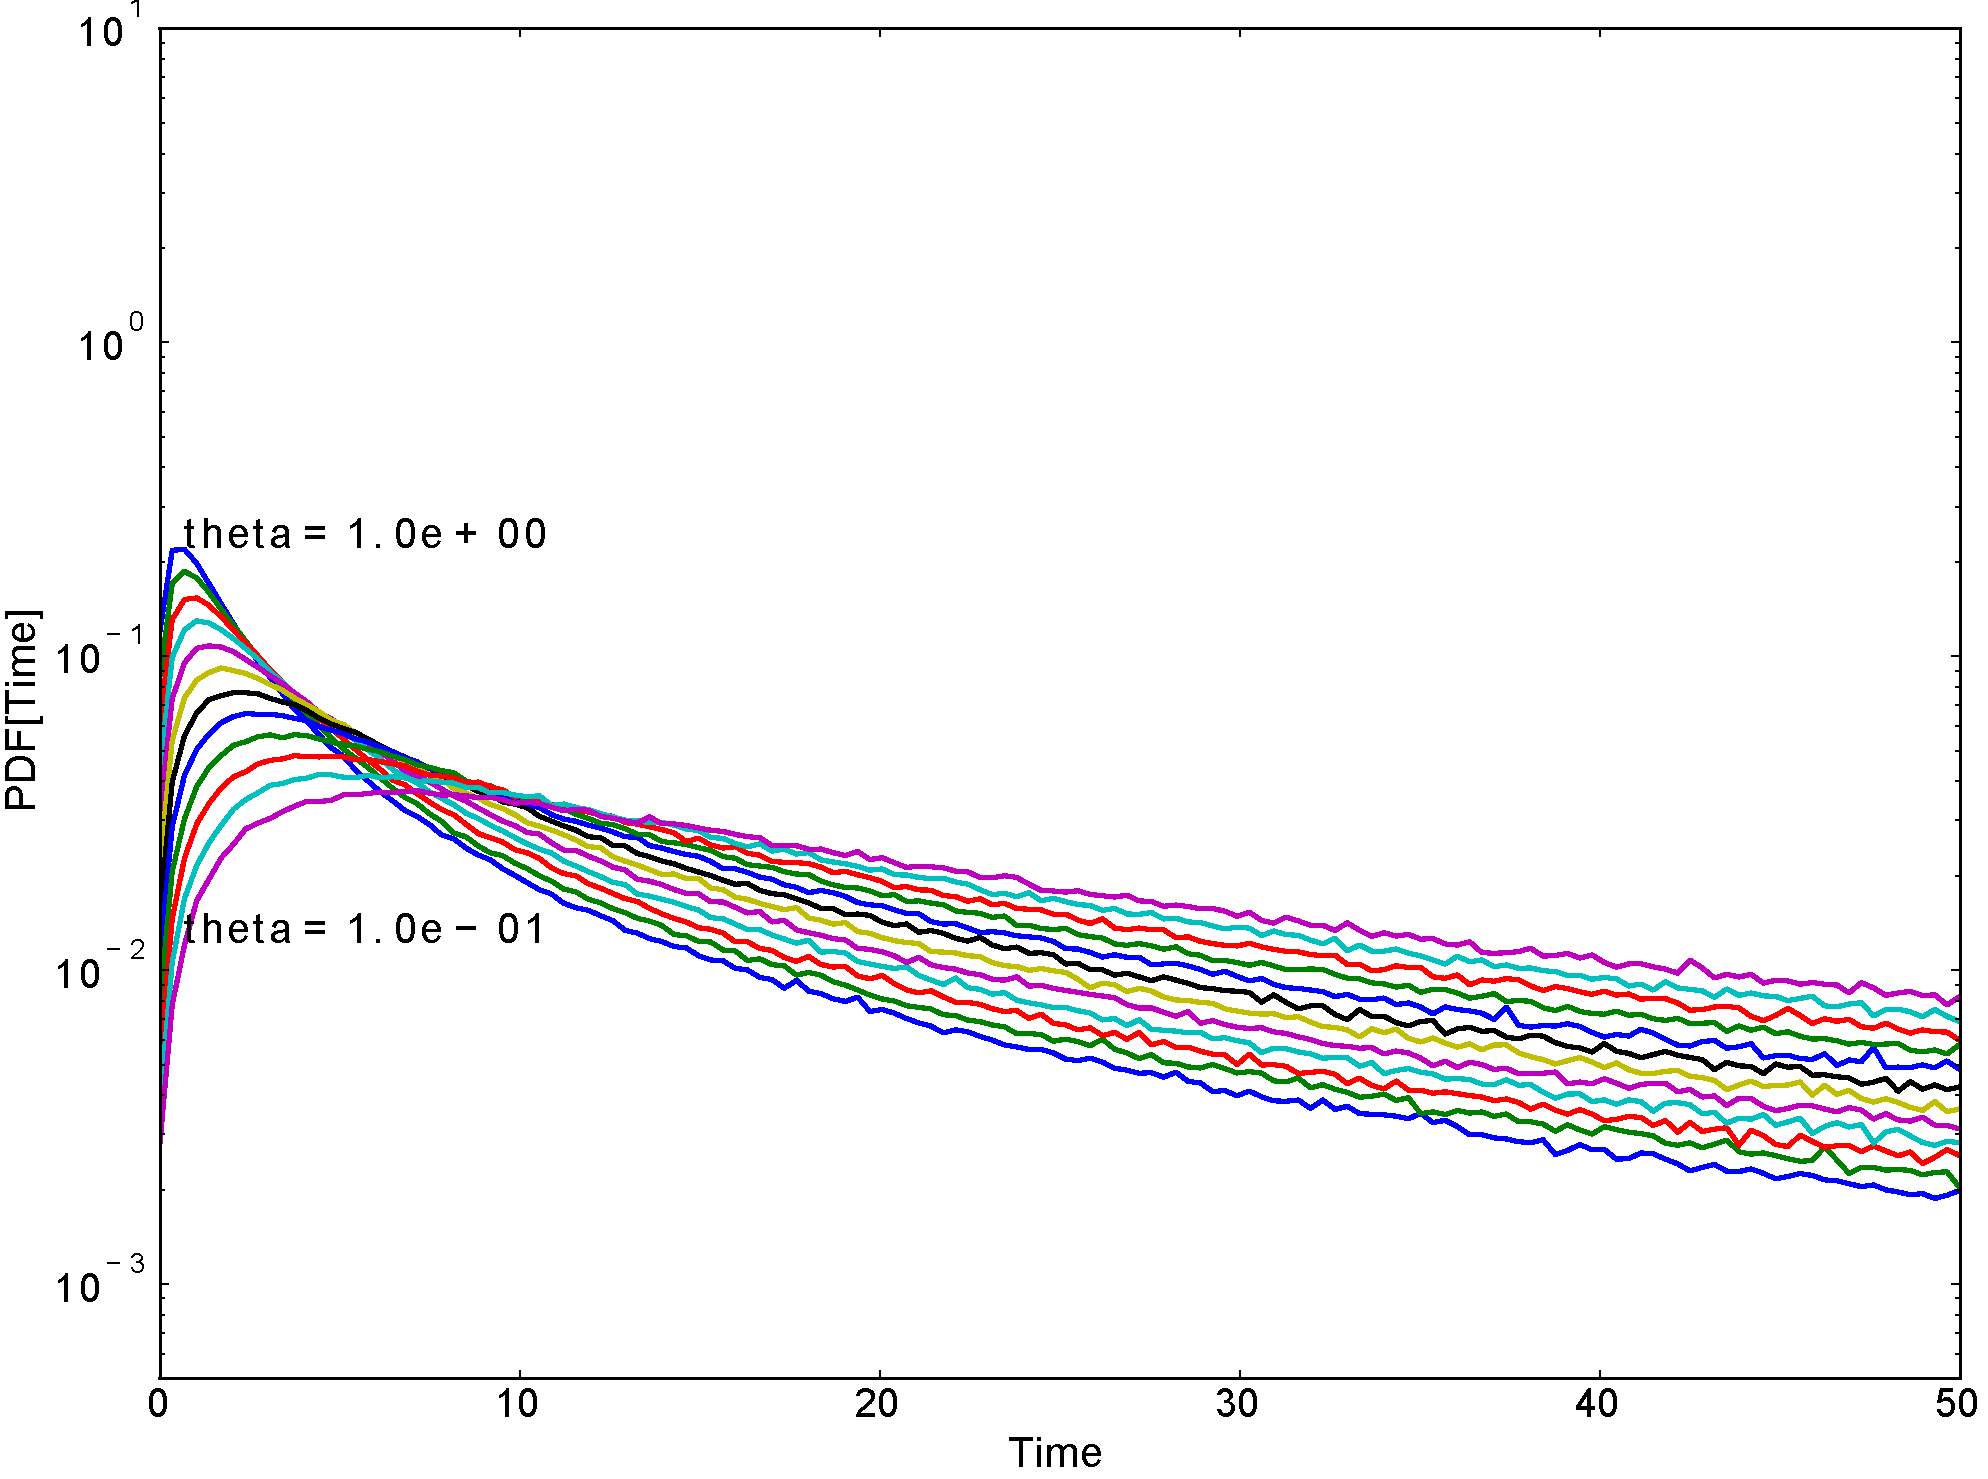
\includegraphics[width=\textwidth,height=\textheight,keepaspectratio]{{supplemental/figures/name_gts_-_ffpilot_phase_zero_dwell_time_dist_-_many_thetas_-_1e6_samples_-_fixed}.pdf}
    \end{center}
    \caption[Phase 0 waiting time distributions for many variants of \abr{GTS}, low accuracy]{Genetic Toggle Switch phase 0 inter-event time distribution for values of $\theta$ in between $.1$ and $10$ (inclusive). $10^6$ samples in each distribution.}
    \label{fig:name_gts_-_ffpilot_phase_zero_dwell_time_dist_-_many_thetas_-_1e6_samples}
\end{figure}
\clearpage

\begin{figure}[h]
    \begin{center}
        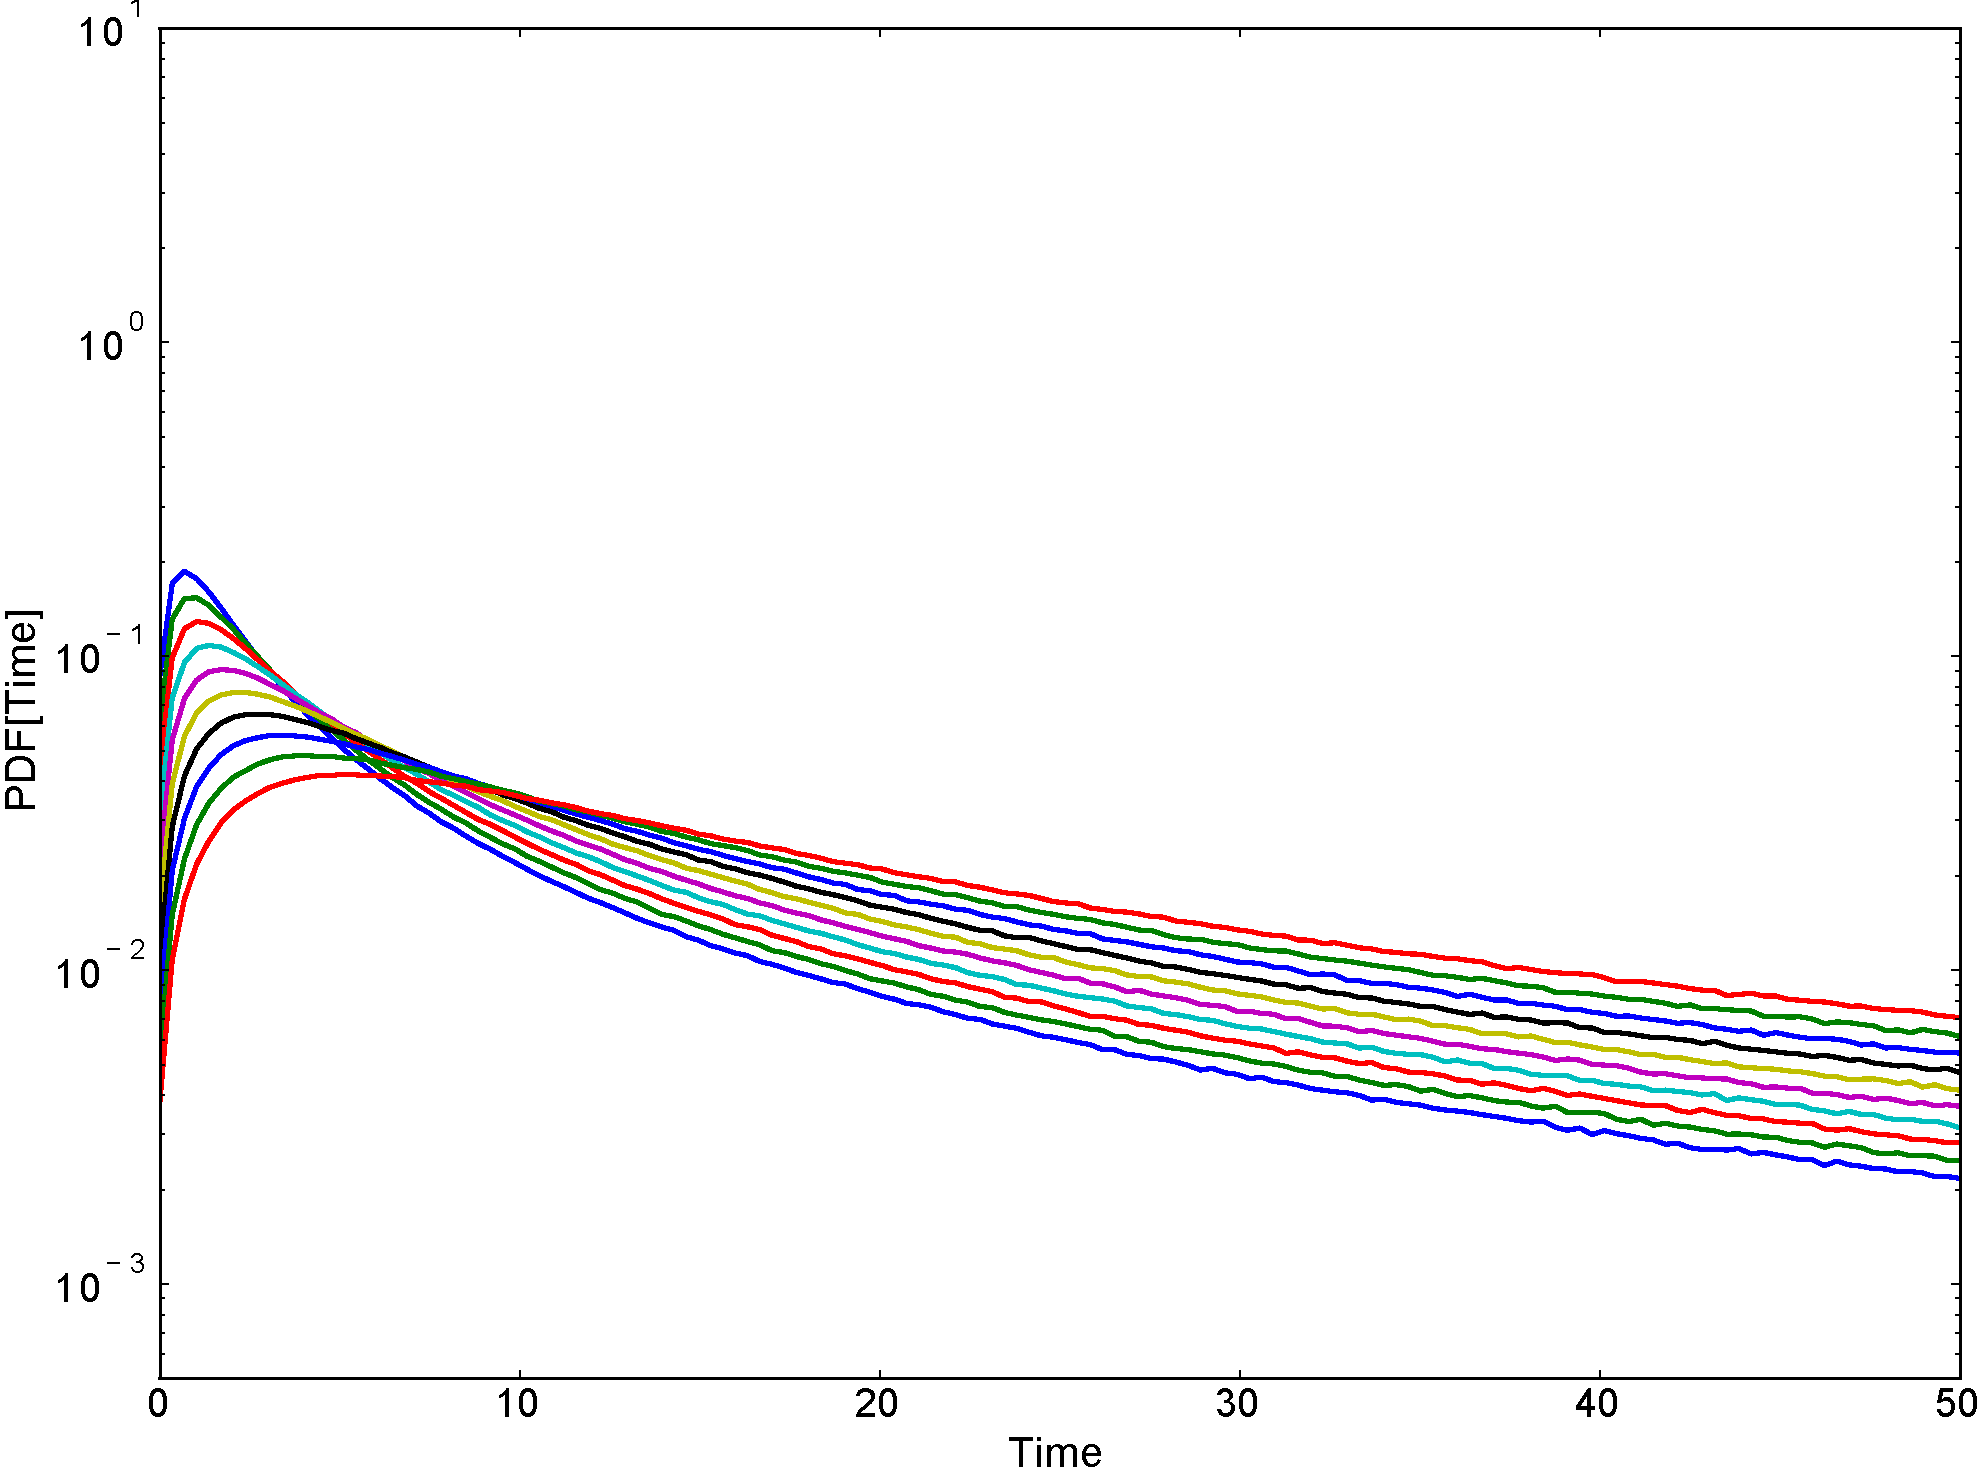
\includegraphics[width=\textwidth,height=\textheight,keepaspectratio]{{supplemental/figures/name_gts_-_ffpilot_phase_zero_dwell_time_dist_-_many_thetas_-_1e7_samples_-_fixed}.pdf}
    \end{center}
    \caption[Phase 0 waiting time distributions for many variants of \abr{GTS}, high accuracy]{Genetic Toggle Switch phase zero inter-event time distribution for values of $\theta$ in between $.1$ and $10$ (non-inclusive). $10^7$ samples in each distribution.}
    \label{fig:name_gts_-_ffpilot_phase_zero_dwell_time_dist_-_many_thetas_-_1e7_samples}
\end{figure}
\clearpage

%\begin{figure}[h]
%    \begin{center}
%        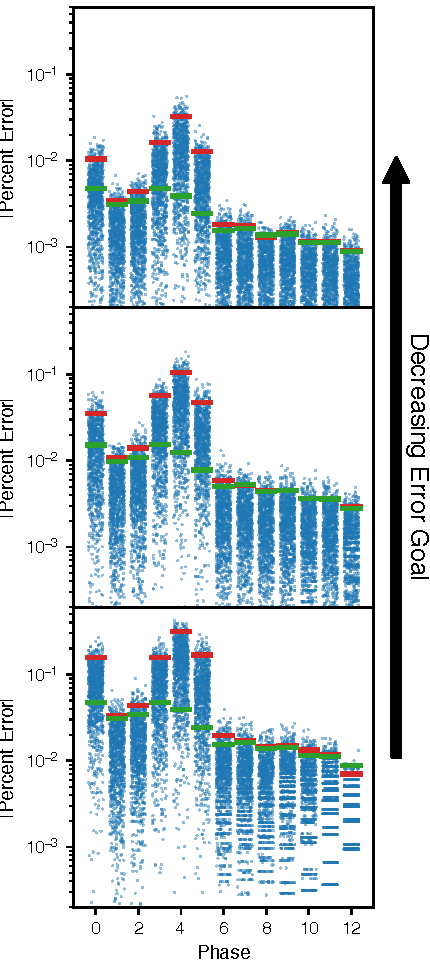
\includegraphics{{Figures/name_gts_-_phase_weight_percent_error_-_error_goal_all_-_pzs_multiplier__1.0e+00_-_theta_1.0e+01}.pdf}
%    \end{center}
%    \caption{Percent error of each phase weight from a set of FFPilot $\GTSSLOWEST$ simulations. The red line marks the 95th percentile of the error. The green line marks the location of the 95th error percentile as predicted by FFPilot at the end of the pilot stage. When the red line is at or below the green line, this means that FFPilot is controlling simulation error as expected.     The same phase zero sampling multiplier, 1X, was used for every simulation. Each subfigure represents results from simulations executed with a different error goal (from top to bottom, 10\%, 3.2\%, and 1\%).}
%    \label{fig:name_gts_-_phase_weight_percent_error_-_error_goal_all_-_pzs_multiplier__1.0e+00_-_theta_1.0e+01}
%\end{figure}
%\clearpage

\begin{figure}[h]
    \begin{center}
        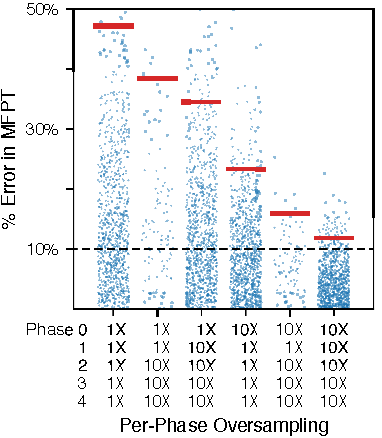
\includegraphics{{supplemental/figures/name_gts_-_stage_fpt_percent_error_-_landscape_fudge_pzs_multiplier_10_-_error_goal_1.0e-01_-_theta_1.0e+01_-_fixed}.pdf}
    \end{center}
    \caption[\abr{FFPilot} simulations of \abr{GTS} executed with various oversampling schemes]{More results from simulations executed with various oversampling schemes. Aside from the use of 10X phase 0 oversampling instead of 20X, these simulations were equivalent to those presented in \figref{fig:name_gts_-_stage_fpt_percent_error_-_landscape_fudge_several_-_error_goal_1.0e-01_-_theta_1.0e+01} in the main paper. As can be seen in the righthand column, 10X oversampling in every phase from 0 to 4 is almost, but not quite, enough to eliminate landscape error. The extent of oversampling in each separate scheme is indicated beneath each column of results. 1X sampling implies that standard number of FFPilot trajectories were sampled in that phase. For purposes of comparison, results from simulations run with no oversampling are included in the first column, and results from simulations run with 10X phase 0, 10X phase 1-4 oversampling are also shown. All simulations were of $\GTSSLOW$ at an error goal of 10\%.}
    \label{fig:name_gts_-_stage_fpt_percent_error_-_landscape_fudge_pzs_multiplier_10_-_error_goal_1.0e-01_-_theta_1.0e+01}
\end{figure}
\clearpage

\begin{figure}[h]
    \begin{center}
        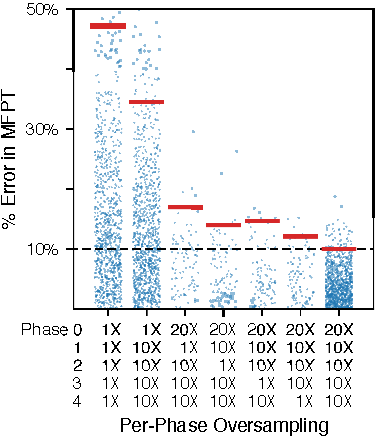
\includegraphics{{supplemental/figures/name_gts_-_stage_fpt_percent_error_-_landscape_fudge_skips_-_error_goal_1.0e-01_-_theta_1.0e+01_-_fixed}.pdf}
    \end{center}
    \caption[\abr{FFPilot} simulations of \abr{GTS} executed with various oversampling schemes, cont]{More results from simulations executed with various oversampling schemes. We wanted to investigate the effects of skipping oversampling in a single phase. Starting at the second column, results are shown from simulations in which we skipped oversampling in phase 0, then in the next column from simulations in which we skipped oversampling in phase 1, and so forth.     The extent of oversampling in each separate scheme is indicated beneath each column of results. 1X sampling implies that standard number of FFPilot trajectories were sampled in that phase. For purposes of comparison, results from simulations run with no oversampling are included in the first column, and results from simulations run with 20X phase 0, 10X phase 1-4 oversampling (which is enough to eliminate landscape error) are also shown. All simulations were of $\GTSSLOW$ at an error goal of 10\%.}
    \label{fig:name_gts_-_stage_fpt_percent_error_-_landscape_fudge_skips_-_error_goal_1.0e-01_-_theta_1.0e+01}
\end{figure}
\clearpage

\begin{figure}[h]
    \begin{center}
        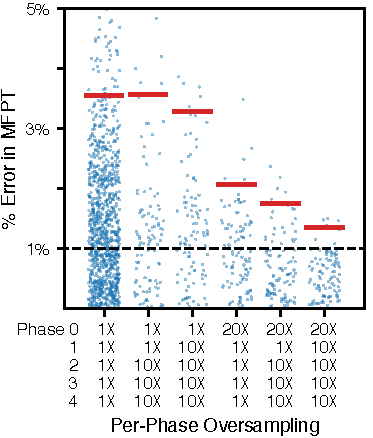
\includegraphics{{supplemental/figures/name_gts_-_stage_fpt_percent_error_-_landscape_fudge_several_-_referenceMFPT_highacc_-_error_goal_1.0e-02_-_theta_1.0e+01_-_fixed}.pdf}
    \end{center}
    \caption[\abr{FFPilot} simulations of \abr{GTS} executed with various oversampling schemes, cont]{$\mfpttrue$ percent errors from a large set of simulations executed with various oversampling schemes. The simulations are similar to those presented in \figref{fig:name_gts_-_stage_fpt_percent_error_-_landscape_fudge_several_-_error_goal_1.0e-01_-_theta_1.0e+01} from the main paper, except that all simulations were of $\GTSSLOW$ at an error goal of 1\% instead of 10\%. All $\mfpttrue$ percent errors are calculated relative to the $\mfpttrue$ value estimated by a high accuracy DS simulation (.62\% error goal).}
    \label{fig:name_gts_-_stage_fpt_percent_error_-_landscape_fudge_several_-_referenceMFPT_highacc_-_error_goal_1.0e-02_-_theta_1.0e+01}
\end{figure}
\clearpage

\begin{figure}[h]
    \begin{center}
        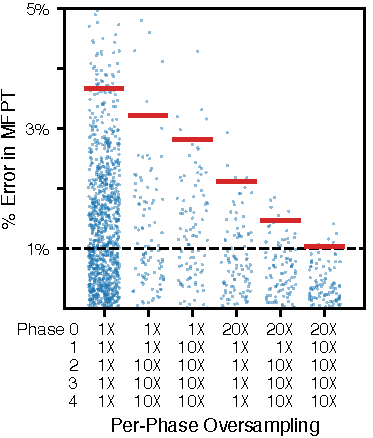
\includegraphics{{supplemental/figures/name_gts_-_stage_fpt_percent_error_-_landscape_fudge_several_-_referenceMFPT_highaccFFPilot_-_error_goal_1.0e-02_-_theta_1.0e+01_-_fixed}.pdf}
    \end{center}
    \caption[\abr{FFPilot} oversampling schemes that achieved the original error goal]{$\mfpttrue$ percent errors from a large set of simulations executed with various oversampling schemes. The simulations are similar to those presented in \figref{fig:name_gts_-_stage_fpt_percent_error_-_landscape_fudge_several_-_error_goal_1.0e-01_-_theta_1.0e+01} from the main paper, except that all simulations were of $\GTSSLOW$ at an error goal of 1\% instead of 10\%. All $\mfpttrue$ percent errors are calculated relative to the $\mfpttrue$ value estimated by a high accuracy FFPilot simulation (.1\% error goal).}
    \label{fig:name_gts_-_stage_fpt_percent_error_-_landscape_fudge_several_-_referenceMFPT_highaccFFPilot_-_error_goal_1.0e-02_-_theta_1.0e+01}
\end{figure}
\clearpage

\begin{comment}
\begin{figure}[h]
    \begin{center}
        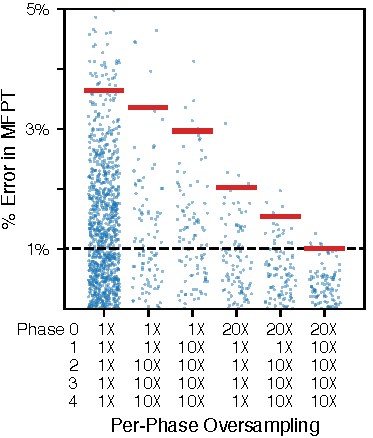
\includegraphics{{supplemental/figures/name_gts_-_stage_fpt_percent_error_-_landscape_fudge_several_-_referenceMFPT_mean_-_error_goal_1.0e-02_-_theta_1.0e+01}.pdf}
    \end{center}
    \caption{$\mfpttrue$ percent errors from a large set of simulations executed with various oversampling schemes. The simulations are similar to those presented in \figref{fig:name_gts_-_stage_fpt_percent_error_-_landscape_fudge_several_-_error_goal_1.0e-01_-_theta_1.0e+01} from the main paper, except that all simulations were of $\GTSSLOW$ at an error goal of 1\% instead of 10\%. In this version of the figure, all $\mfpttrue$ percent errors are calculated relative to the mean $\mfpttrue$ value estimated by all of the simulations within that particular oversampling condition.}
    \label{fig:name_gts_-_stage_fpt_percent_error_-_landscape_fudge_several_-_referenceMFPT_mean_-_error_goal_1.0e-02_-_theta_1.0e+01}
\end{figure}
\clearpage    
\end{comment}

\begin{figure}[h]
    \begin{center}
        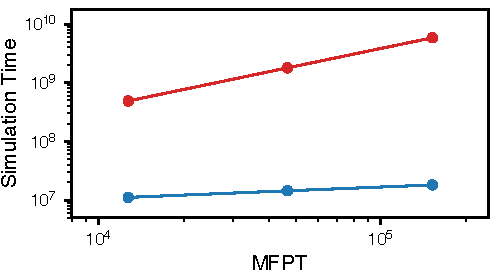
\includegraphics{{supplemental/figures/name_h_-_speedup_plot_-_simtime_vs_mfpt_-_error_goal_1.0e-02_-_fixed}.pdf}
    \end{center}
    \caption[Simulation time vs \abr{MFPT} for several \abr{SRG} models]{Simulation time vs \abr{MFPT} for several \abr{SRG} models. The simulation time for both \abr{DS} (red lines) and \abr{FFPilot} (blue lines) are shown.} 
    \label{fig:name_h_-_speedup_plot_-_simtime_vs_mfpt_-_error_goal_1.0e-02}
\end{figure}
\clearpage

\begin{figure}[h]
    \begin{center}
        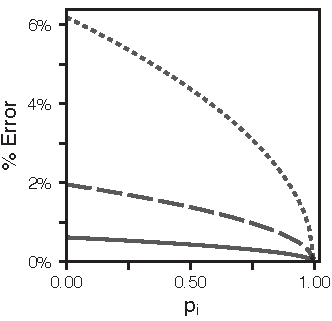
\includegraphics{{supplemental/figures/blind_optimization_-_percent_error_vs_pi_-_several_success_counts_-_fixed}.pdf}
    \end{center}
    \caption[Maximum error when using the blind optimization method of the \abr{FFPilot} pilot stage]{Maximum error (with respect to a single phase weight, 95\% confidence) vs phase weight for a phase $\phasegz$ when using the blind optimization method from the \abr{FFPilot} pilot stage. Each of the lines shows the error for a different fixed value of the successful trajectory count, $\successcount = \samplecountpilot$. (solid line) $\samplecountpilot = 10^5$, (dashed line) $\samplecountpilot = 10^4$, (dotted line) $\samplecountpilot = 10^3$.}
    \label{fig:blind_optimization_-_percent_error_vs_pi_-_several_success_counts}
\end{figure}
\clearpage

\begin{figure}[h]
    \begin{center}
        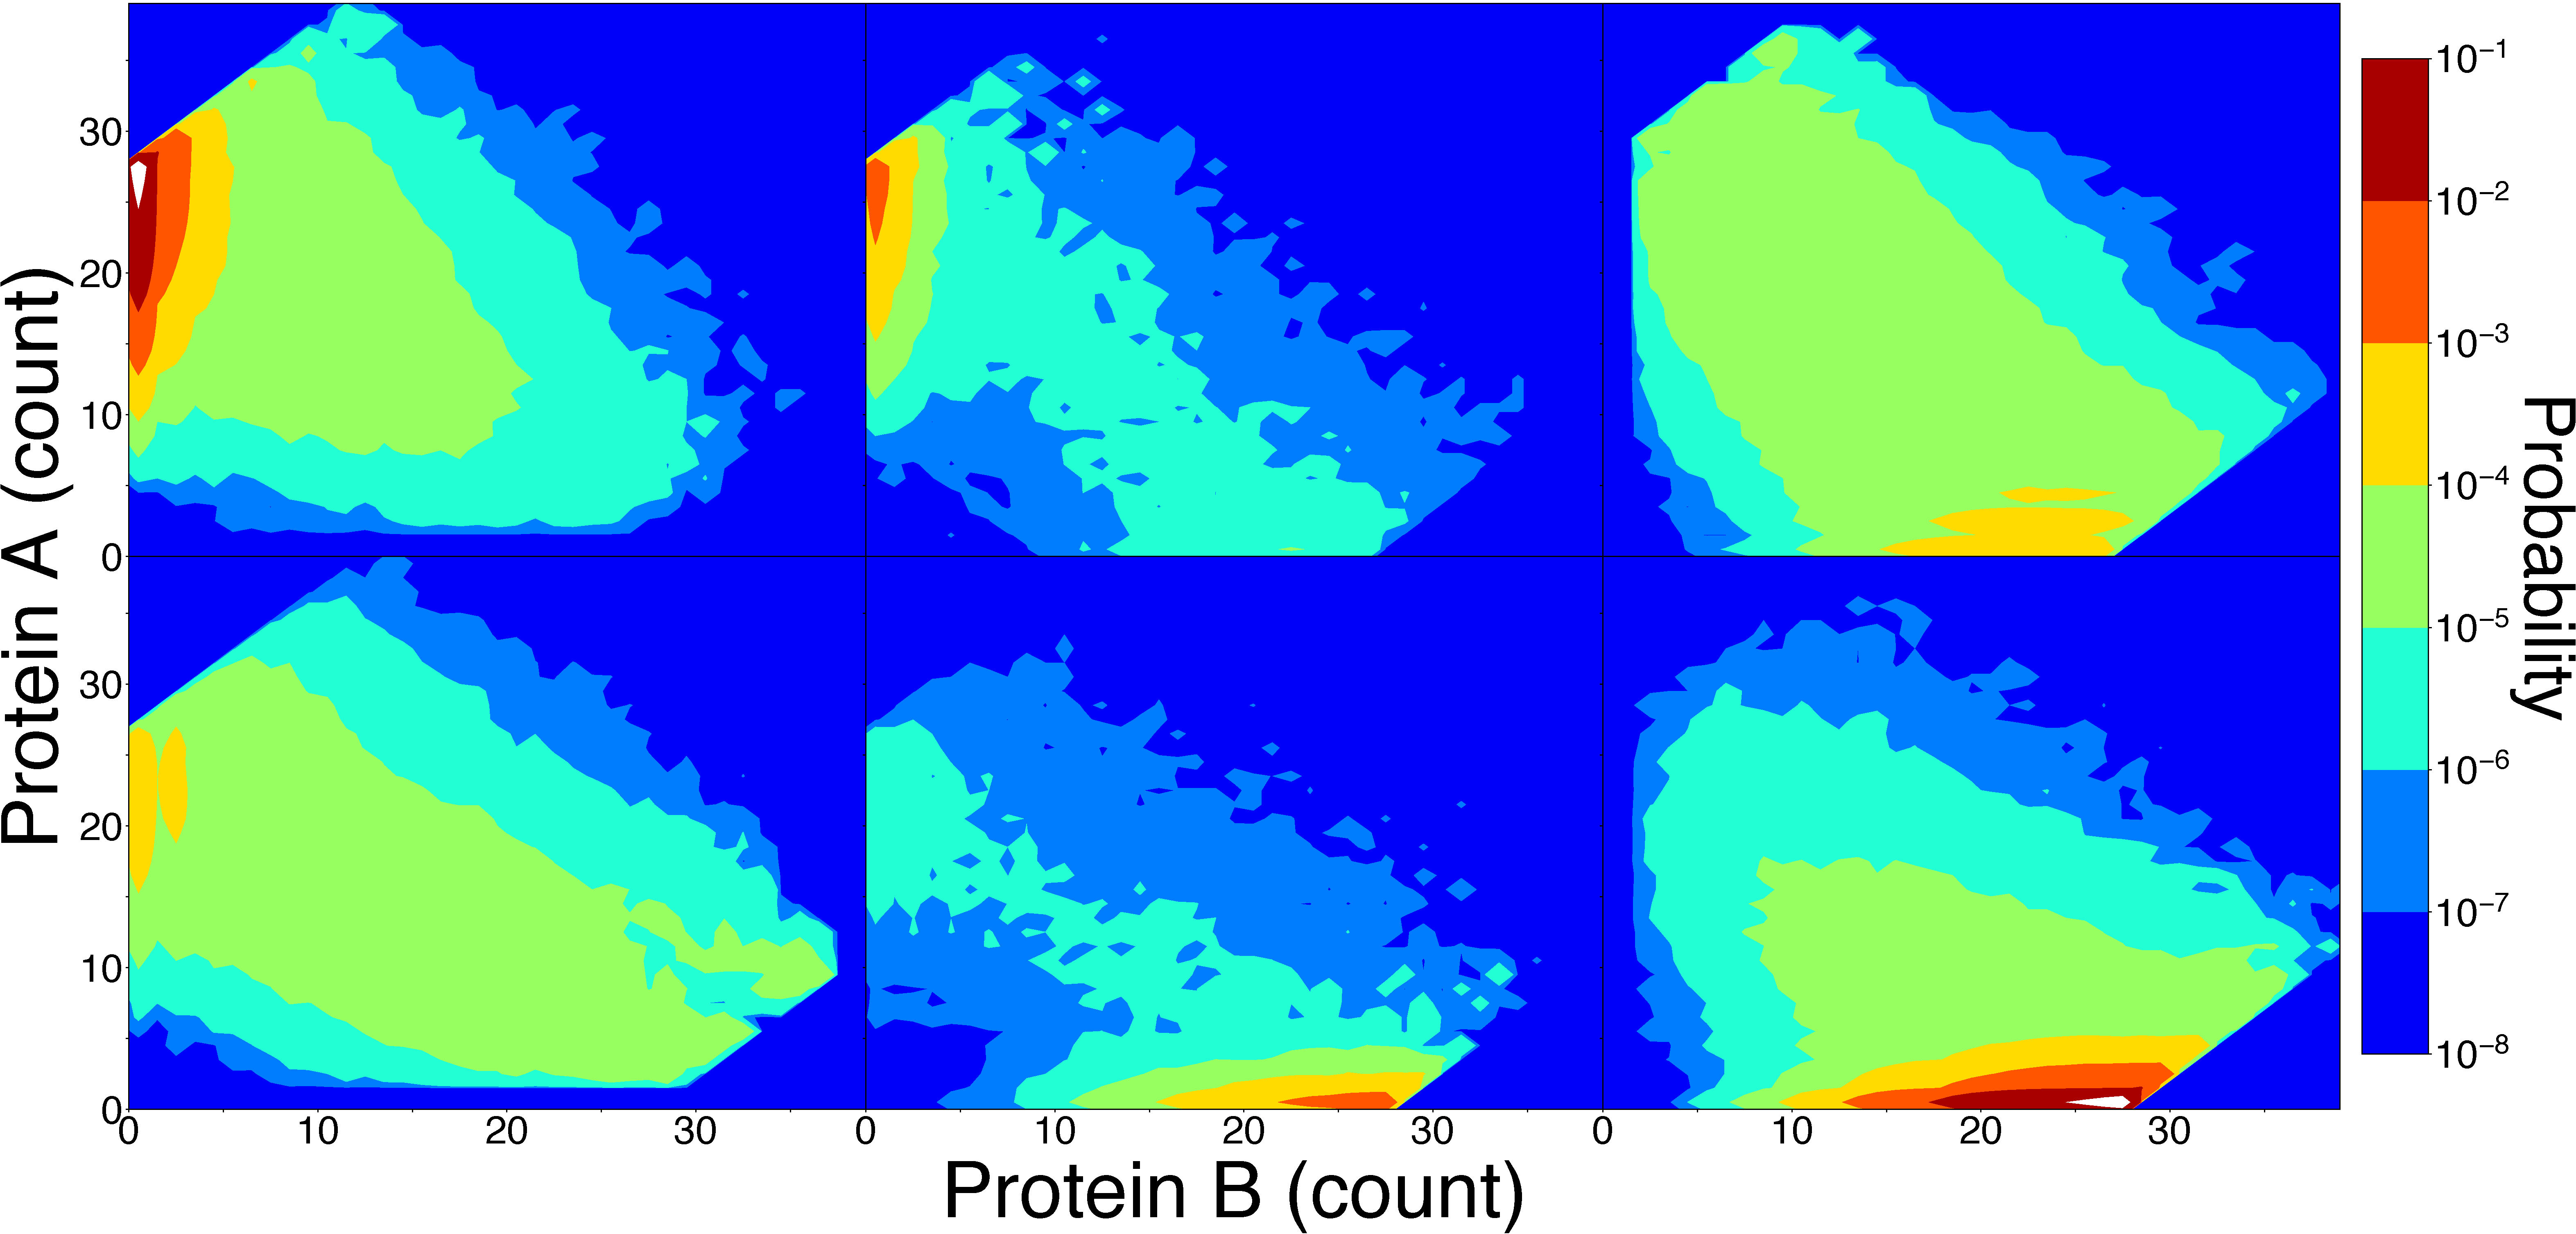
\includegraphics[width=\textwidth,height=\textheight,keepaspectratio]{{supplemental/figures/name_gts_-_landscape_operator_slices_-_plot_contour_-_fixed}.pdf}
    \end{center}
    \caption[The state landscape of $\GTSSLOW$, sliced by operator occupancy]{The state landscape of $\GTSSLOW$, sliced by operator occupancy. The lefthand column shows the slice of the landscape in which an A dimer is bound to the operator DNA, the middle column shows the slice in which the operator is unbound, and the righthand column shows the slice in which the operator is bound to a B dimer. The top row is from a simulation of $\GTSSLOW$ in which it switched $\atob$, and the bottom row is from a simulation in which it switch $btoa$. Complex, high dimensional, and reasonably accurate landscapes can be produced in a straightforward fashion from relatively low cost \abr{FFPilot} simulations. The 3 landscapes in each row represent the output of a single \abr{FFPilot} simulation run to a 10\% error goal, which ran to completion on a laptop in ~5 minutes. The landscapes were analyzed and plotted using LMA, an analysis package written in Python and designed to work alongside the Lattice Microbes simulation suite.}
    \label{fig:name_gts_-_landscape_operator_slices_-_plot_contour}
\end{figure}
\clearpage

%\end{document}


%\documentclass[class=article, float=false, crop=false]{standalone}
%\documentclass[10pt,letterpaper]{article}
%
%\input{error_control_of_enhanced_sampling-header}
%
%\begin{document}

\continuesupplemental

\subsection{Supplemental tables}
\begin{table}[h]
    \caption[Deterministic ordinary differential equation model of the \gtsabbrev{}]{\label{tab:gts_odes}Deterministic ordinary differential equation model of the \gtsabbrev{}.}
    \newcolumntype{Z}{>{\centering\arraybackslash}X}%
    \begin{tabularx}{\textwidth}{Z}
        \hline\hline
        \text{Deterministic Genetic Toggle Switch Equations} \\
        \hline
        {\begin{align*}
            \frac{d\gtsa}{dt}   &= -10 \gtsa^2 + 10 \gtsaa + \theta \left( -\frac{\gtsa}{4} + \gtsoaa + \gtso \right) \\
            \frac{d\gtsaa}{dt}  &= 5 \gtsa^2 + \gtsoaa - 5 \gtsaa \left( \gtso + 1 \right)                            \\
            \frac{d\gtsoaa}{dt} &= -\gtsoaa + 5 \gtsaa \cdot \gtso                                                    \\
            \frac{d\gtsb}{dt}   &= -10 \gtsb^2 + 10 \gtsbb + \theta \left( -\frac{\gtsb}{4} + \gtsobb + \gtso \right) \\
            \frac{d\gtsbb}{dt}  &= 5 \gtsb^2 + \gtsobb - 5 \gtsbb \left( \gtso + 1 \right)                            \\
            \frac{d\gtsobb}{dt} &= -\gtsobb + 5 \gtsbb \cdot \gtso                                                    \\
            \frac{d\gtso}{dt}   &= 1 - \gtsoaa - \gtsobb
        \end{align*}} \\
        \hline\hline
    \end{tabularx}
\end{table}
\clearpage

%\end{document}




%\end{document}
